\documentclass[format=acmsmall]{acmart}
%\documentclass[sigconf]{acmart}

%%% Some recommended packages.
%\usepackage{booktabs}   %% For formal tables:
%                        %% http://ctan.org/pkg/booktabs
%\usepackage{subcaption} %% For complex figures with subfigures/subcaptions
%                        %% http://ctan.org/pkg/subcaption
\newif\iffull
\fullfalse

\usepackage{mathptmx}
\usepackage{graphicx}
\usepackage{mathtools}
\usepackage{amsmath}
\usepackage[utf8]{inputenc}
\usepackage{cleveref}
\usepackage{listings}
\usepackage{array}
\usepackage{breqn}
\usepackage{tikz}
\usepackage{algorithmicx}
\usepackage[Algorithm,ruled]{algorithm}
\usepackage{algpseudocode}
\usepackage{pifont,xspace}
\usetikzlibrary{automata,positioning,shapes.geometric}
\newcommand{\name}{{\sc Zeppelin}\xspace}
\newcommand{\Name}{\name}
\newcommand{\genesis}{Genesis\xspace}
\newcommand{\pushcode}[1][1]{\hskip\dimexpr#1\algorithmicindent\relax}
\newcolumntype{P}[1]{>{\centering\arraybackslash}p{#1}}

\usetikzlibrary{calc}
\usetikzlibrary{arrows}
\usetikzlibrary{decorations.markings}

\newcommand*{\StrikeThruDistance}{0.2cm}%
\newcommand*{\StrikeThru}{\StrikeThruDistance,\StrikeThruDistance}%


\tikzset{strike thru arrow/.style={
		decoration={markings, mark=at position 0.5 with {
				\draw [black, thick,-] 
				++ (-\StrikeThruDistance,-\StrikeThruDistance) 
				-- ( \StrikeThruDistance, \StrikeThruDistance);}
		},
		postaction={decorate},
	}}
	

\usepackage{times}
\usepackage[font=small]{caption}
%\usepackage{subcaption}
\usepackage{enumitem}
%\usepackage{usenix}
\usepackage{epsfig}
%\usepackage[TABBOTCAP]{subfigure}
\usepackage{color}
%\usepackage{thumbpdf}
\usepackage{verbatim}
%\usepackage{hyperref}
\usepackage{url}
%\usepackage{booktabs}
\usepackage{colortbl}
\usepackage{enumitem}
\usepackage[export]{adjustbox}
\usepackage{subfig}
\usepackage{mathtools}
\usepackage{amssymb}
\usepackage{amsthm}
\usepackage{multirow}% http://ctan.org/pkg/multirow
\usepackage{multicol}
\usepackage{hhline}
\usepackage{wrapfig}
\usepackage{array,ragged2e}
\newcommand{\minisection}[1]{\smallskip\noindent{\bf #1.}}
\newcommand{\secref}[1]{{\S\ref{#1}}}
\newcommand{\secsref}[2]{{Sections~\ref{#1} and \S\ref{#2}}}
\newcommand{\figsref}[2]{{Figure~\ref{#1} and \ref{#2}}}
\newcommand{\appref}[1]{{Appendix~\ref{#1}}}
\newcommand{\thmref}[1]{{Theorem~\ref{#1}}}
\newcommand{\lemref}[1]{{Lemma~\ref{#1}}}
\newcommand{\corref}[1]{{Corollary~\ref{#1}}}
\newcommand{\proref}[1]{{Property~\ref{#1}}}

\newcommand{\compactcaption}[1]{\vspace{-1em}\caption{#1}\vspace{-1em}}
\newcommand{\botcompactcaption}[1]{\caption{#1}\vspace{-1em}}
\newcommand{\topcompactcaption}[1]{\vspace{-1em}\caption{#1}\vspace{-0.5em}}

\newenvironment{compactitemize}
{
   \begin{itemize}[leftmargin=1.5em]
   \vspace{-1ex}
   \setlength{\topsep}{0pt}
   \setlength{\itemsep}{0em}
   \setlength{\parskip}{0pt}
   \setlength{\parsep}{0pt}
}
{
   \vspace{-1ex}
   \end{itemize}
}
\newenvironment{compact2itemize}
{
	\begin{itemize}[leftmargin=1.5em]
		\vspace{-1ex}
		\setlength{\topsep}{0pt}
		\setlength{\itemsep}{0.5em}
		\setlength{\parskip}{0pt}
		\setlength{\parsep}{0pt}
	}
	{
		\vspace{-1ex}
	\end{itemize}
}


\newenvironment{compactenumerate}
{
   \begin{enumerate}[leftmargin=1.5em]
   \vspace{-1ex}
   \setlength{\topsep}{0pt}
   \setlength{\itemsep}{0em}
   \setlength{\parskip}{0pt}
   \setlength{\parsep}{0pt}
}
{
   \vspace{-1ex}
   \end{enumerate}
}

\ifdefined\commentenabled
    \newcommand{\loris}[1]{\textcolor[rgb]{0.00,0.00,1.00}{L: #1}}
    \newcommand{\aditya}[1]{\textcolor[rgb]{0.00,0.00,1.00}{A:#1}}
    \newcommand{\kausik}[1]{\textcolor[rgb]{0.2,0.80,0.2}{K: #1}}
    \newcommand{\aaron}[1]{\textcolor[rgb]{0.00,0.2,0.6}{AGJ: #1}}
\else
    \newcommand{\loris}[1]{}
    \newcommand{\aditya}[1]{}
    \newcommand{\kausik}[1]{}
    \newcommand{\aaron}[1]{}
\fi

\newcommand{\ARC}{ARC\xspace}
\newcommand{\ARCs}{ARCs\xspace}

\usepackage[medium, compact]{titlesec}
%\usepackage[font={bf,small}]{caption}
%\usepackage{titlesec}
\titlespacing*{\section}{1pt}{3.5pt}{2pt}
\titlespacing*{\subsection}{1pt}{3pt}{1.5pt}
\titlespacing*{\subsubsection}{1pt}{3pt}{1.5pt}
%\newtheorem{example}{Example}
%\newtheorem{theorem}{Theorem}[section]
%\newtheorem{lemma}{Lemma}[section]
\lstset{
	basicstyle=\itshape,
	xleftmargin=2em,
	literate={->}{$\rightarrow$}{2}
	{α}{$\alpha$}{1}
	{δ}{$\delta$}{1}
}

\crefname{Section}{§}{§§}
\Crefname{Section}{§}{§§}

\usepackage{color}
\newcommand{\loris}[1]{\textcolor[rgb]{0.00,0.00,1.00}{#1}}
\newcommand{\aditya}[1]{\textcolor[rgb]{1.00,0.00,0.00}{AA:#1}}
\newcommand{\kausik}[1]{\textcolor[rgb]{0.00,0.5,0.5}{K: #1}}
\newcommand{\todo}[1]{{\color{red}{\bf TODO: #1}}}

\usepackage{float}

\newcommand{\cL}{{\cal L}}

\setlength{\textfloatsep}{6pt}

\settopmatter{printacmref=false,printfolios=true}



% \TODO : Uncomment
\setcopyright{acmcopyright}
\acmJournal{POMACS}
\acmYear{2018} \acmVolume{2} \acmNumber{1} \acmArticle{22} \acmMonth{3} \acmPrice{$15.00$}
\acmDOI{10.1145/3179425}

%% Bibliography style



\begin{document}
%% Title information
\title{Synthesis of Fault-tolerant Distributed Router Configurations}         %% [Short Title] is optional;
                                        %% when present, will be used in
                                        %% header instead of Full Title.    
                                        %% can be repeated if necessary;
                                        %% contents suppressed with 'anonymous'
%\subtitle{Subtitle}                     %% \subtitle is optional
%\subtitlenote{with subtitle note}       %% \subtitlenote is optional;
                                        %% can be repeated if necessary;
                                        %% contents suppressed with 'anonymous'


%% Author information
%% Contents and number of authors suppressed with 'anonymous'.
%% Each author should be introduced by \author, followed by
%% \authornote (optional), \orcid (optional), \affiliation, and
%% \email.
%% An author may have multiple affiliations and/or emails; repeat the
%% appropriate command.
%% Many elements are not rendered, but should be provided for metadata
%% extraction tools.
\author{Kausik Subramanian}
\author{Loris D'Antoni}
\author{Aditya Akella}
\affiliation{
\institution{University of Wisconsin-Madison}            %% \institution is required
\streetaddress{1210 W Dayton St}
\city{Madison}
\state{WI}
\postcode{53706}
\country{USA}
}
\email{sskausik08@cs.wisc.edu}          %% \email is recommended
\email{loris@cs.wisc.edu}
\email{akella@cs.wisc.edu}
% \author{Loris D'Antoni}
% \affiliation{
% \institution{University of Wisconsin-Madison}            %% \institution is required
% \streetaddress{1210 W Dayton St}
% \city{Madison}
% \state{WI}
% \postcode{53706}
% \country{USA}
% }
% \email{loris@cs.wisc.edu}          %% \email is recommended

% \author{Aditya Akella}
% \affiliation{
% \institution{University of Wisconsin-Madison}   %% \institution is required
% \streetaddress{1210 W Dayton St}
% \city{Madison}
% \state{WI}
% \postcode{53706}
% \country{USA}
% }         
% \email{akella@cs.wisc.edu}          %% \email is recommended



  {\bf Abstract---} Operators in multi-tenant cloud datacenters
  require support for diverse and complex end-to-end policies, such
  as, reachability, middlebox traversals, isolation, traffic
  engineering, and network resource management. We present \Name, a
  datacenter network management system which allows policies to be
  specified in a declarative manner without explicitly programming the
  network data-plane.  \name tackles the problem of enforcing policies
  by synthesizing switch forwarding tables. It uses the formal
  reasoning foundations of constraint solving in combination with fast
  off-the-shelf SMT solvers.  To improve synthesis performance, \Name
  incorporates a novel search strategy that uses regular expressions
  to specify properties that leverage the structure of datacenter
  networks,
%topologies to specify properties of the path 
  and a divide-and-conquer synthesis procedure which exploits the
  structure of policy relationships.  We have prototyped \Name, and conducted
  experiments with a variety of workloads on real-world topologies
  to demonstrate its  performance.
  %% Overall, the approach used by \Name is general and instrumental
  %% to building a comprehensive network management system.



%  \begin{CCSXML}
% <ccs2012>
% <concept>
% <concept_id>10003033.10003083.10003098</concept_id>
% <concept_desc>Networks~Network manageability</concept_desc>
% <concept_significance>500</concept_significance>
% </concept>
% </ccs2012>
% \end{CCSXML}

% \ccsdesc[500]{Networks~Network manageability}

\keywords{Zeppelin; Synthesis; Fault Tolerance; Network Management; Routing protocols;
Hierarchical network control plane}


%% \maketitle
%% Note: \maketitle command must come after title commands, author
%% commands, abstract environment, Computing Classification System
%% environment and commands, and keywords command.


\maketitle

% The default list of authors is too long for headers.
\renewcommand{\shortauthors}{K. Subramanian et al.}

\section{Introduction}
%% Conventionally, a network primarily acted as a backbone for
%% communication among machines, and these communications used the
%% ``shortest" path in the network based on certain metrics for deciding
%% the path between two machines.  Today,

Many enterprises are increasingly migrating their on-premise IT
infrastructure to cloud datacenters. In such environments, the
different enterprises (tenants) share different resources, such as,
the compute machines that run their applications and network
infrastructure used for communication among these applications.
Operators of such multi-tenant datacenters thus have to deal with a
multitude of machines communicating with each other (flows) over a
network that is composed of many tens to hundreds of routers or
switches (devices)~\cite{mpa-imc15}. With growing diversity of
enterprise applications and the need for security and compliance,
these pathways of communication through the datacenter network are
subject to increasingly complex network-based policies.

Consider an enterprise tenant in such a datacenter. She may desire
basic communication among her applications along shortest paths based
on certain metrics (reachability). In addition, she may wish that
traffic attempting to reach some of her applications be examined by a
set of ``middleboxes'' for auditing and access control
(traversal). Another tenant may additionally desire a subset of her
flows not share any infrastructure with others' flows for strong
security or Quality-of-Service considerations (isolation).  In
parallel, cloud operators must meet key operational objectives. For
instance, they often need to optimize network performance objectives
(traffic engineering), e.g., minimizing the maximum load imposed by
all tenants on network links, and deal with resource constraints such
as link capacity bounds and switch table sizes. Also, since datacenter
networks are highly prone to link/switch
failures~\cite{datacenterfailures}, operators need to gracefully
transition the old (pre-failure) dataplane to a policy-compliant new
(post-failure) one in a rapid and/or efficient manner.

Today, configuring network devices to implement these complex policies
and objectives in aggregate is manual, ad-hoc, and error-prone.  This
can lead to misconfigurations and violations of tenant service-level
agreements (SLAs) which can have a severe performance and security
impact.

%%  However, in real-life, the
%% process of policy enforcement by network operators is manual and
%% ad-hoc, leading to violations of service-level agreements and
%% mis-configurations which have severe performance and security
%% impacts. With the boom in cloud services, datacenter networks deal
%% with thousands of flows which are not constant, but in flux, thus,
%% making it difficult to enforce them in an ad-hoc manner.

%% Network operators desire various different end-to-end policies to
%% support in clouds and enterprise networks. Tenants or organisations
%% require support for basic policies like reachability between hosts,
%% and specifying different middlebox policies for certain
%% flows. Operators, on top of that require support for complex policies
%% like traffic isolation between flows to provide fairness and
%% specifying resource constraints like link bandwidth and switch table
%% sizes to perform traffic engineering and network resource management.

The rise of \emph{software-defined networking} (SDN) has allowed
operators to program networks in a more intuitive manner. In SDN, a
general-purpose centralized controller machine (control plane)
controls end-to-end communication pathways by managing network
forwarding rules on a collection of programmable switches (data
plane). Using a global view of current network topology, the
controller can program forwarding rules on switches based on
application requirements.
%However, many existing SDN
%frameworks are too low-level, 
%making it challenging 
%to write controller applications using these which generate 
% the data plane enforcing the above policies. %% For many
%% of the policies, generating the data plane is an NP-complete problem
%% and requires the design of efficient custom heuristics; combining
%% different policies' heuristics together is non-trivial.
Unfortunately, existing SDN programming languages (e.g.,
Frenetic~\cite{frenetic} and Pyretic~\cite{pyretic}) are too
constraining: operators would ideally want to specify and realize
policies/objectives network-wide, whereas these languages focus on programming
{\em individual} switch behaviors.  Moreover, for many types of
policies, generating a data plane that enforces them is a
%  an NP-complete 
computationally hard problem, requiring the design of efficient custom
heuristics {\em per policy/objective type}. Other recent works on
network-wide policy enforcement~\cite{merlin,simple} go beyond the
single-switch model, but they target specific types of policies/objectives and
thus are difficult to extend to other commonly desired policy types
(e.g., isolation).
%; combining  different policies' heuristics together is non-trivial. 
 %% \aditya{we need to be
% careful
%%   not to bin all SDN languages into this switch-by-switch model}
%% \kausik{Do you want to make changes here?}







%% support
%% other kinds of policies such as traffic isolation.

%%  like
%% joint bandwidth provisioning and waypoint routing in Merlin
%% \cite{merlin}, and middlebox policy enforcement in SIMPLE
%% \cite{simple} or FlowTags~\cite{flowtags}. However, these approaches

In this paper, we seek a {\em general} approach that allows a variety
of rich policies/objectives to be specified as the input, with the output being
the corresponding set of switch forwarding rules such that the
complexities of correctly realizing the policies in the data plane are
hidden from operators. This is an important step toward {\em
  intent-based networking}~\cite{intent}, where operators specify {\em
  what} they want the network to do instead of worrying about {\em
  how} the network must be configured.
%their networks. %% To support a cornucopia of policies, an
%% important feature is \emph{generality} of the approach of policy
%% enforcement, so that it can be extended to enforce custom policies
%% required by the operator.
This paper makes a case for using \emph{data plane synthesis} as a
practical approach to realizing this vision in the multi-tenant
datacenter context.
%% switch
%% table forwarding rules to the solve the problem of policy enforcement
%% by use of off-the-shelf SMT-solvers.

We present \Name, a framework for {\em declaratively} specifying and
enforcing complex policies and objectives such as, isolation,
middlebox traversals and failure resilience. To tackle the high
complexity of enforcing some of these policies (for e.g., enforcing
isolation is NP-complete), \Name encodes the problem as that of
constraint solving and leverages recent advances in fast
Satisfiability Modulo Theories (SMT) solvers to efficiently search for
a solution to the constraints.  The solution is then translated into
switch forwarding rules.
%Using SMT solvers with 
%support for linear optimization, \name can perform traffic engineering, and
%minimal network repair. We extend \name to synthesize
%resilient switch tables to \emph{proactively} ensure policy-compliance
%in failure scenarios. 
%% This
%% paper presents Genesis, a
%% network management tool where the network operators can express the
%% network-wide policies in a high-level declarative manner and Genesis
%% will synthesize the lower-level switch forwarding rules for realising
%% these policies, eliminating the need for operators to work on
%% switch-level behaviours. 
By leveraging the formal guarantees of constraint solving, \Name
eliminates the room for error in the enforcement of complex
policies and objectives.

%\kausik{Do we need to make the point of sacrificing performance for generality for POPL? }

Unfortunately, due to the the large space of forwarding plane
configurations, naively encoding policies using SMT solvers results in
slow synthesis speeds (up to hundreds-thousands of seconds in the
median case; \secref{sec:baselineeval}) which can be impractical.
%enterprise networks today because the space of forwarding plane configurations
%is huge. 
To make synthesis more practical, \Name leverages domain-specific
properties to simplify the constraints handled by the SMT solver.
We allow the network operator to write restricted
forms of regular expressions, called \emph{tactics}, that blacklist
paths based on certain patterns that are not desired in a datacenter
network.
%\loris{how about: ...based on path patterns that are not desired...}
These tactics are used to discard several constraints, 
acting as a search strategy for the solver.
%\aditya{the previous sentence is vague}
%By identifying a restricted syntax for specifying
%tactics, we 
Tactics can improve the synthesis procedure and achieve
%constraints added to the solver without additional constraints
%required to ensure the solution satisfies the tactic and achieve
a 1.5$\times - $400$\times$ speedup 
(median speedup: 1.6$\times$, average speedup: 22$\times$).

 Secondly, we develop a \emph{divide-and-conquer} synthesis procedure
 that leverages the relationships among  isolation policies to
 improve synthesis performance. The procedure partitions the input
 policies into effective components such that \name can synthesize
 these components separately and faster than the complete problem.
 Divide-and-conquer synthesis can halve the synthesis time for 40\% of
 synthetic isolation workloads.
 %% which vary in size and complexity
 %% of isolation.
 %\aditya{is this statement correct? what is 40\% of scenarios?}
 %\aditya{the
   %previous sentence is vague} 

%% are
%% huge, and by supporting a set of diverse and complex policies with
%% different search objectives, we require to create a model general and
%% expressive enough to support these. This poses a challenge as to can
%% synthesis performance be improved by leveraging knowledge specific to
%% the problem of policy enforcement in networks?

%We implement \Name using ... We evaluate it using .... Key highlights .... \aditya{all of these are todo}.\kausik{Do we need a para or will the next para suffice?}
\noindent \textbf{Contributions.} \ \ \ Our contributions are the following.
\begin{compactitemize}
\item An extensible declarative framework for describing
  complex policies/objectives and a modular SMT-based algorithm for enforcing policies and objectives
  like isolation, waypoints (\secref{sec:synthesisalgo}), traffic engineering~(\secref{sec:optimization}), and 
  failure resiliency (\secref{sec:resiliency});
\item A modified synthesis algorithm based on tactics, which leverages datacenter network structure
  to blacklist undesirable path patterns (\secref{sec:tactic});
\item A divide-and-conquer procedure for speeding up synthesis by leveraging the 
structure of policy interactions (\secref{sec:optimistic});
\item An implementation of \Name and an extensive evaluation on
  different policy/objective workloads, topologies and multi-tenancy
  settings (\secref{sec:evaluation}).
		%to quantify the performance of Genesis. 
\end{compactitemize}
%\aditya{todo}

\iffull\else
A long version
of this paper containing all the proofs has been submitted as supplementary material.
\fi
%% : We present the design and implementation of a network management
%% system with support for a diverse set of complex end-to-end
%% policies like isolation, waypoints and capacity. We designed a
%% novel search strategy using regular expressions to prune the space
%% of forwarding plane configurations by leveraging the network
%% structure to provide properties of the path, especially in
%% datacenter topologies. Lastly, we design a heuristical synthesis
%% routine leveraging the nature of policy interactions to improve
%% synthesis performance.

%\section{Motivation}
\begin{figure}
	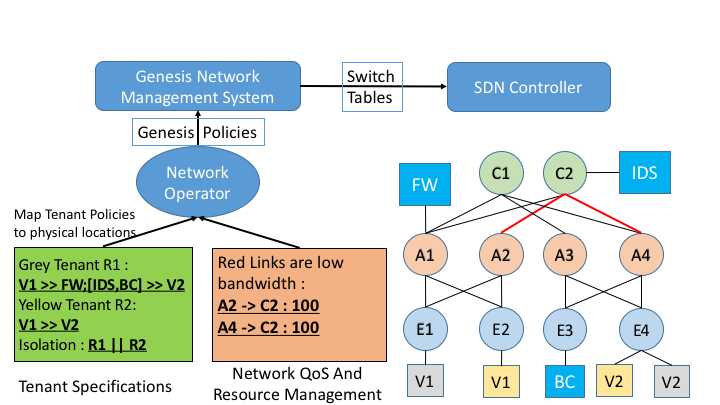
\includegraphics[height=7.5cm,right]{figures/architecture.png}
	\caption{Rough layout of system architecture. Also will come up with an example figure here.}
	\label{fig:architecture}
\end{figure}
In this section, we describe the type of policies that tenants and
network operators may wish to realize. %% For simplicity, we assume a
%% multi-tenant cloud set up, where both the tenants and the provider
%% wish to realize policies over their respective networks. However,
%% these policies, and our framework, are applicable to other settings,
%% e.g., enterprise networks with different departments imposing
%% different sets of policies.
We use Figure XXX as a running example. This figure shows several
tenants who differ in the nature of policies they wish to realize. We
note that these policies reflect and, in some cases, extend the
policies that enterprises realize in their on-site networks today as
well as policies that data center operators support for the different
workloads they host~\cite{mpa-imc15}.  The policies include:

\aditya{explain the figure here}.
\kausik{Will do this now}

\aditya{define flow, flow group, policy etc here}
% \aditya{need to start by saying we focus on multi-tenant clouds, although our system can apply elsewhere too}

% Operators of enterprise and multi-tenant clouds deal with policy
% requirements of different organisations and tenants, as well as
% require support to manage the network for providing QoS guarantees and
% network resource management internally, invisible to the
% tenants. Network operators need to be able to express complex policies
% in an intuitive declarative fashion, and the network management system
% must derive the individual switch forwarding behavior without
% involving the operator.


\begin{itemize}
\item \textbf{Reachability}: This enables network communication
  between specific groups of a tenant's virtual cloud instances,
  applications, or hosts. \aditya{refer here to an example in the
    figure}
\item \textbf{Middlebox traversals}: A tenant may wish that traffic
  between two of her endpoints, or from another tenant, must traverse
  through specific middleboxes (locations, or logical descriptors) for
  security, access control or performance reasons. This can be
  specified via an ordered sequence of sets of middleboxes for a flow
  group to traverse, where the middleboxes in a set can be traversed
  in any order, but all middleboxes in the set must be traversed.  The
  unordered set abstraction leverages the fact that middleboxes
  without dependencies in their traffic processing behavior can be
  placed in any order in a service chain~\cite{pga}. Thus the
  middlebox traversal specification outlined here generalizes the
  notion of a service chain.  \aditya{refer here to an example in the
    figure}

  %% \aditya{refer here to an example in
  %%   the figure} In several cases \loris{how true is this?} the order
  %% in which these middle-boxes is traversed is not relevant and the
  %% policy language should therefore support unordered waypoints.

\item \textbf{Isolation}: Tenants may require various QoS guarantees
  that enforce varying degrees of isolation for their traffic. In the
  extreme, a tenant could ensure that her flow groups are not affected
  by any other tenant by strictly isolating the path of the tenant's
  flows from others' flows. \aditya{refer here to an example in the
    figure} A tenant could also specify isolation for a subset of her
  (performance-sensitive) flows from other flows of her own deployment
  or those belonging to other tenants; the rest of the tenants' flows
  mayy require no guarantees.

%%   There has been a rising emergence of 
%% multi-tenant clouds, which is more economical for tenants to use
%% rather than managing their own private datacenters. However,
%% the current Service Level Agreements (SLAs)
%% provided to tenants are centered around compute, storage, or
%% external traffic bandwidth. Lack of guarantees on the network
%% between tenant instances leads to unpredictability of performance
%% for distributed applications. Also, multi-tenant clouds are
%% susceptible to attacks on the network by malicious tenants who could
%% hog the internal network bandwidth, or conduct side-channel
%% attacks~\cite{heyyou-ccs}.
% Conventionally,
% this problem is mitigated by static rate-limiting, but it can lead
% to under-utilisation of resources.
%% Cloud provider can offer (paying) tenants various QoS guarantees
%% that enforce varying degrees of tenant isolation. In the extreme,
%% this could ensure that a tenant's performance is not affected by
%% any other tenant by strictly isolating the path of tenant's flows
%% from others' flows. \aditya{refer here to an example in
%% 	the figure} The tenant could also specify isolation for certain
%%  performance-sensitive flows, while the rest of the tenant-flows
%%   would be without guarantees with varying degrees of pricing. 
%%   Thus, support for isolation is an important feature in multi-tenant 
%%   networks. 
 \end{itemize}
%TODO : MODIFY Synthesis of waypoints to support logical waypoints
%% Since, cloud tenants do not have a view of the actual physical
%% topology, the policy requirements for tenants are at a coarser level
%% of control. While support for the above policies can be used to satisfy tenant
%% SLAs, network operators can benefit from a fine-grained
%% control of network resources, integrated with support for tenant specifications 
%% for effective management of the network. \newline

\textbf{Network Resource Management}: While support for the above
policies can be used to satisfy tenant SLAs, network operators can
benefit from a fine-grained control of network resources, integrated
with support for tenant specifications for effective management of the
network. For instance, to aid traffic enginerring, the network
operator may specify policies constraining the maximum number of
tenant flows that can traverse a given link or sets of links in the
network. She may also wish to ensure traffic from some sensitive
applications does not contend for bandwidth on constrained links with
elastic traffic from batch applications.
          %% capacity
          %% of certain links such that tenant flows using the link do
          %% not exceed the capacity of the link. Such policies can be
          %% useful to ensure the low bandwidth links are not used by
          %% more tenants such that their performance is affected and
          %% can be used to provide bandwidth guarantees to tenants.
  Likewise, to tackle hardware heterogeniety, operators can specify
  switch constraint policies, like the size of the rule table to
  restrict the number of flows traversing a particular switch or set
  of switches.
%\item \textbf{Network Maintenance}: \aditya{this whole para does not
%    parse and needs updating} Operators on a regular basis perform link and
%  switch maintenances, and need to ensure that during maintenance, the network still
%  conforms to the SLAs of the tenants and resource capacity
%  policies.   \aditya{the following sentence does not make sense} Using Genesis, the operator
%  can specify the links and switches that will be down for maintenance, and Genesis can synthesize 
%  the rules for the updated network with all policies satisfies, which then can be pushed to 
%  the network before maintenance. 
%\end{itemize}

  Our goal is to design a system that allows the above policies to be
  specified in a simple, declarative manner, and abstracts away 
  data plane enforcement and the intricacies thereof.
  
\subsection{Synthesis} \label{sec:synthesis} 

\begin{table}[!t]
\begin{small}
	\begin{center}
		\begin{tabular}{m{7.8em}  m{15.9em} } 
			{\bf Policy} & {\bf Description} \\ 
			\hline
			Reachability & There is a path from router $src$ to router $dst$ for destination $\lambda$ \\ \hline
			Reachability with \newline Ordered Waypoints & The path  from $src$ to $dst$ for destination $\lambda$ 
			traverses some switch in the set $W_1$, \ldots, then some switch in the set $W_k$.\\ \hline
			Traffic Isolation & Paths of two reachability policies $R1$ and $R2$ do not share  links \\ \hline
			Traffic Engineering  & Minimize total/max link utilization \\
		\end{tabular}
	\end{center}
	\compactcaption{\genesis path-based policy support.} \label{tab:policysupport} 
\end{small}
\end{table}


%\section{Policy Support} \label{sec:policy}
%We design a language GPL (Genesis Policy Language) for network operators to express the desired end-to-end policies in a declarative manner which is interpreted by the Genesis synthesizer to find the forwarding rules for the network topology which enforce the input policies (\cref{fig:arch}). Genesis supports the following policies : 
%% Figure of GPL's syntax
%\begin{enumerate} 
%	\item \textbf{Reachability}: $predicate : src >> dst$ \\
%	This policy specifies the packets satisying $predicate$ have ingress router $src$ and egress router $dst$, and requires rules forwarding packets satisfying $predicate$ from $src$ to $dst$. There must be no forwarding loops in the network. 
%	\item \textbf{Waypoint}: $predicate : src >> W >> dst$ \\
%	The waypoint policy is a stronger reachability policy, and specifies that packet satisfying $predicate$ with ingress router $src$ and egress router $dst$ must pass through the set of waypoints $W$ in no particular order. The waypoint policy helps operators and tenants to specify the middleboxes the packets must traverse through without worrying about order, or having to use header tags to enforce a particular order \cite{flowtags}. 
%	\item \textbf{Traffic Isolation}:  $R1 \ || \ R2$ \\
%	The traffic isolation policy ensures that the . This policy can be used to provide fairness guarantees, since the paths of $R1$ and $R2$ don't share a link, the bandwidth used by $R1$ will not affect the bandwidth used by $R2$ and vice-versa. The condition of sharing a link in the same direction is due to the fact that links are full-duplex so, traffic flowing in one direction is not affected by the traffic flowing in the other direction.
%	\item \textbf{Security Isolation}: $R1 <> R2$ \\
%	The security isolation policy is stronger than the traffic isolation policy, and ensures that the path of the reachabiltiy/waypoint policies $R1$ and $R2$ do not share a link in both directions for increased security.
%	\item \textbf{}: $sw_1 \rightarrow sw_2 : capacity$ \\
%	The link capacity policy specifies that the capacity for link $sw_1 \rightarrow sw_2$ is $capacity$, and the weights of flows traversing the link in the direction of $sw_2$ do not exceed the capacity of the link.  
%	\item \textbf{Switch Table Size}: $sw : size$ \\
%	The router table size policy is used to specify the size of the forwarding table of the router $sw$ and ensures that the number of flows traversing through $sw$ does not exceed $size$ as each flow would require a forwarding rule at the switch.
%\end{enumerate}



Providing support for realizing the complex set of policies using
existing SDN programming languages like Pyretic and Frenetic is
challenging, because these policies are global and cannot be enforced
by programming individual behaviour of switches. Existing network
management systems provide support for complex policies including
middlebox placement and bandwidth constraints~\cite{}; however these
are tailor-made for certain policies and lack generality and
extensibility.

We design a general network management system that realizes the above
sets of policies by performing {\em synthesis} of switch forwarding
rules to enforce end-to-end policies. The system architecture of \name
is shown in \cref{fig:architecture} and the way in which policies
outlined in the previous section can be specified in \name is shown in
Table~\ref{tab:policysupport} .

Unlike previous efforts in the synthesis space (see~\cite{}), \Name is
not tailored to specific formalisms such as regular expressions and
this aspect makes it modular and easily extensible.
%and allows to devise specific
%techniques for each type of policies. 
To draw an analogy with SMT solvers, \Name can be seen as a constraint
solver that allows the addition different types of policies
(respectively, the theories in SMT) and that allows the design of
different types of optimizations based on the properties desired by cloud
  operators using \Name. 
  
Our work is motivated by recent progress in program synthesis.
Program synthesis is defined as the task of discovering an executable
program from user intent expressed in the form of some
constraints. There are three key dimensions to synthesis: the kind of
constraints that it accepts as expression of user intent, the space of
programs over which it searches, and the search technique it
employs. Program synthesis has seen limited applications to networks,
specifically to controller synthesis~\cite{netegg}, where the idea is
to learn from examples and synthesize the behavior of individual
switches (e.g., learning switches or firewalls); furthermore, this
technique applies to networks operating in a reactive mode (where the
first packet of a connection is processed by the controller to
determine the actions to employ). Like Frenetic~\cite{} and
Pyretic~\cite{}, this switch-centric approach is too constraining.

\Name\ leverages synthesis at a high level as follows: given a set of
policies which describe user intent, the search space is the space of
all forwarding plane configurations and the search technique involved
is SAT/SMT solving. The solution found is implemented by installing
the necessary switch rules via a skeleton controller.

This approach is appealing for a variety of different reasons: 

(1)
Policies useful to operators are \emph{proactive} (i.e., they are not
dependent on the actual packet flow), and our synthesis approach
naturally aligns with such proactive policies.

%  and this enables enforcing policies by synthesis
% of switch-table rules, and using a skeleton SDN controller to deploy
% the forwarding rules to the switches. In contrast, in trying to
% synthesize reactive policies (like a firewall), the controller needs
% to store the state of flows it has received and have a control module
% following the specifications \aditya{huh? this doesn't make sense...},
% which is an interesting synthesis problem, but orthogonal to our
% approach.

(2) Correct policy enforcement is challenging due to different
objectives for each of the policies - ensuring isolation between flows
may lead to overshooting capacity and vice-versa - and is a common
cause of incorrect configurations in networks.  Our approach removes
the need for a verification step in which the operator has to
``check'' whether an attempted configuration meets the desired
policies.  By using a formal reasoning technique, we are able to
consider the space of all forwarding configurations and find a
solution which is \emph{correct by construction}, i.e., it adheres to
satisfying a diverse set of policies, eliminating the room for error
by the network operator.

(3) Automatically enforcing policies is a task with
\emph{high theoretical complexity}. 
For example, enforcing isolation policies
is as hard as solving
graph-coloring, a well-known
NP-complete problem (see \cref{sec:isolationNP} for the proof).
%, which means
%that any system solving this would need to exhaustively search the
%space of all forwarding plane configurations. 
Many search techniques can be used to find the forwarding rules when
handling a particular class of policies, but when multiple types of
policies are combined (isolation, middlebox traversal, capacity
constraints), devising good search techniques becomes challenging.
Thanks to the many engineering efforts, SMT solvers abstract away most
of this complexity and allow us to unify the search objectives for
every policy into a generalized search technique.
%Thus, by reducing this problem to a SMT instance and
%leveraging fast off-the-shelf SMT solvers developed over years of
%research, \Name can provide support for diverse policies required by
%network operators. 
Crucially, \Name can be extended with ease to
support new policies without requiring changes to the search
techniques to find the solution.
%% \loris{I would like to convey that we are in some sense a Network solver module policy,
%% in the sense that we support theories (the policies) and now people can work on engineering
%% the solver for different classes of policies.
%% }
%% \kausik{To flow from this subsec to the next? Support for policies is 
%% 	inbuilt, but operators can engineer tactics to suit their needs. Is this what you want to convey?}
%% \loris{I found many words used to address the same concept:
%% enforce the policies, synthesize rules, etc...
%% try to be uniform or it's quite hard to understand what is being done.
%% } 
%% \kausik{I think "enforce policies" would be better? The title explains the rest.}

\subsection{Performance Challenges} \label{sec:performance}

One of the key challenges of \Name is the synthesis
performance. 
Due to the rich  policies supported by \Name
finding a consistent set of switch forwarding rules 
has exponential time worst case complexity in
the number of policies.
Moreover, since policies such as isolation affect
the paths many different flows, it is not possible to incrementally synthesize
the forwarding rules corresponding to each flow. 
Despite the recent advances in SMT solvers, to make
the synthesis problem feasible in practice,
there is a need to improve the performance of the solver
using techniques that are specific to the network domain.
\loris{I rewrote this previous paragraph}


In this paper, we propose various techniques leveraging
\emph{domain-specific} knowledge to improve synthesis performance. We
propose the idea of \emph{tactics} (\cref{sec:tactic}), which are
search strategies leveraging the network structure of datacenter
topologies, to specify properties of the paths for the reachability
policies.  Tactics are a way for network operators to specify a
high-level constraint on the set of paths allowed for reachability
policies.  Path properties are expressed using a simplified form of
regular expressions which, after being converted into a finite
automata, can be used to simplify the set of constraints provided to
the solver.  In particular, one can eliminate constraints that cannot
be true for any of the paths accepted by the automaton language. We
find that this can result in \aditya{XXX} speedup. \aditya{fill this
  in!} 


Another property of datacenter topologies is that the huge
interconnect of links can lead to multiple solutions to the problem
(i.e., to enforce the policies provided).  To take advantage of this
property, we design a heuristic procedure called \emph{optimistic}
synthesis (\cref{sec:optimistic}) which leverages the structure of
isolation policy interactions among tenants to partition the input
policies into effective components and synthesize these components
faster than the complete problem. To improve the effectiveness of the
heuristic, whenever the SMT solver fails to find a solution we extract
the unsatisfiability core produced by the SMT solver and 
add it to our set of constraints to quickly converge to a correct solution.
Informally, the unsatisfiability core can be viewed
as a set of constraints that describes why there wasn't a feasible solution~\cite{}. 
\loris{I rewrote this, should add a citation to something discussing unsat core}


%!TEX root = paper.tex
\section{Overview}
Before formally defining the problem tackled by \name and the algorithms, 
we present an overview of \name using an end-to-end
example. Consider the hierarchical network in \Cref{fig:example} which
is split into three OSPF domains, and these domains communicate
using BGP. Host A talks to hosts B and C with the following policies:
traffic to B must go through a firewall at router $R_3$, traffic to C 
goes through an IDS at $R_5$ and traffic 
to B and C do not share any links (We discuss the policies supported in
detail in \Cref{sec:policy}). \name 
synthesizes OSPF and BGP router configurations satisfying the 
policies. Illustrating our two-phase approach (\Cref{fig:architecture}), 
\name first uses Genesis to find policy-compliant paths (indicated by the blue and
red paths). Note that there exists multiple solutions for the given
policies, we show how the control plane is synthesized using one of the solutions:
\begin{figure}
	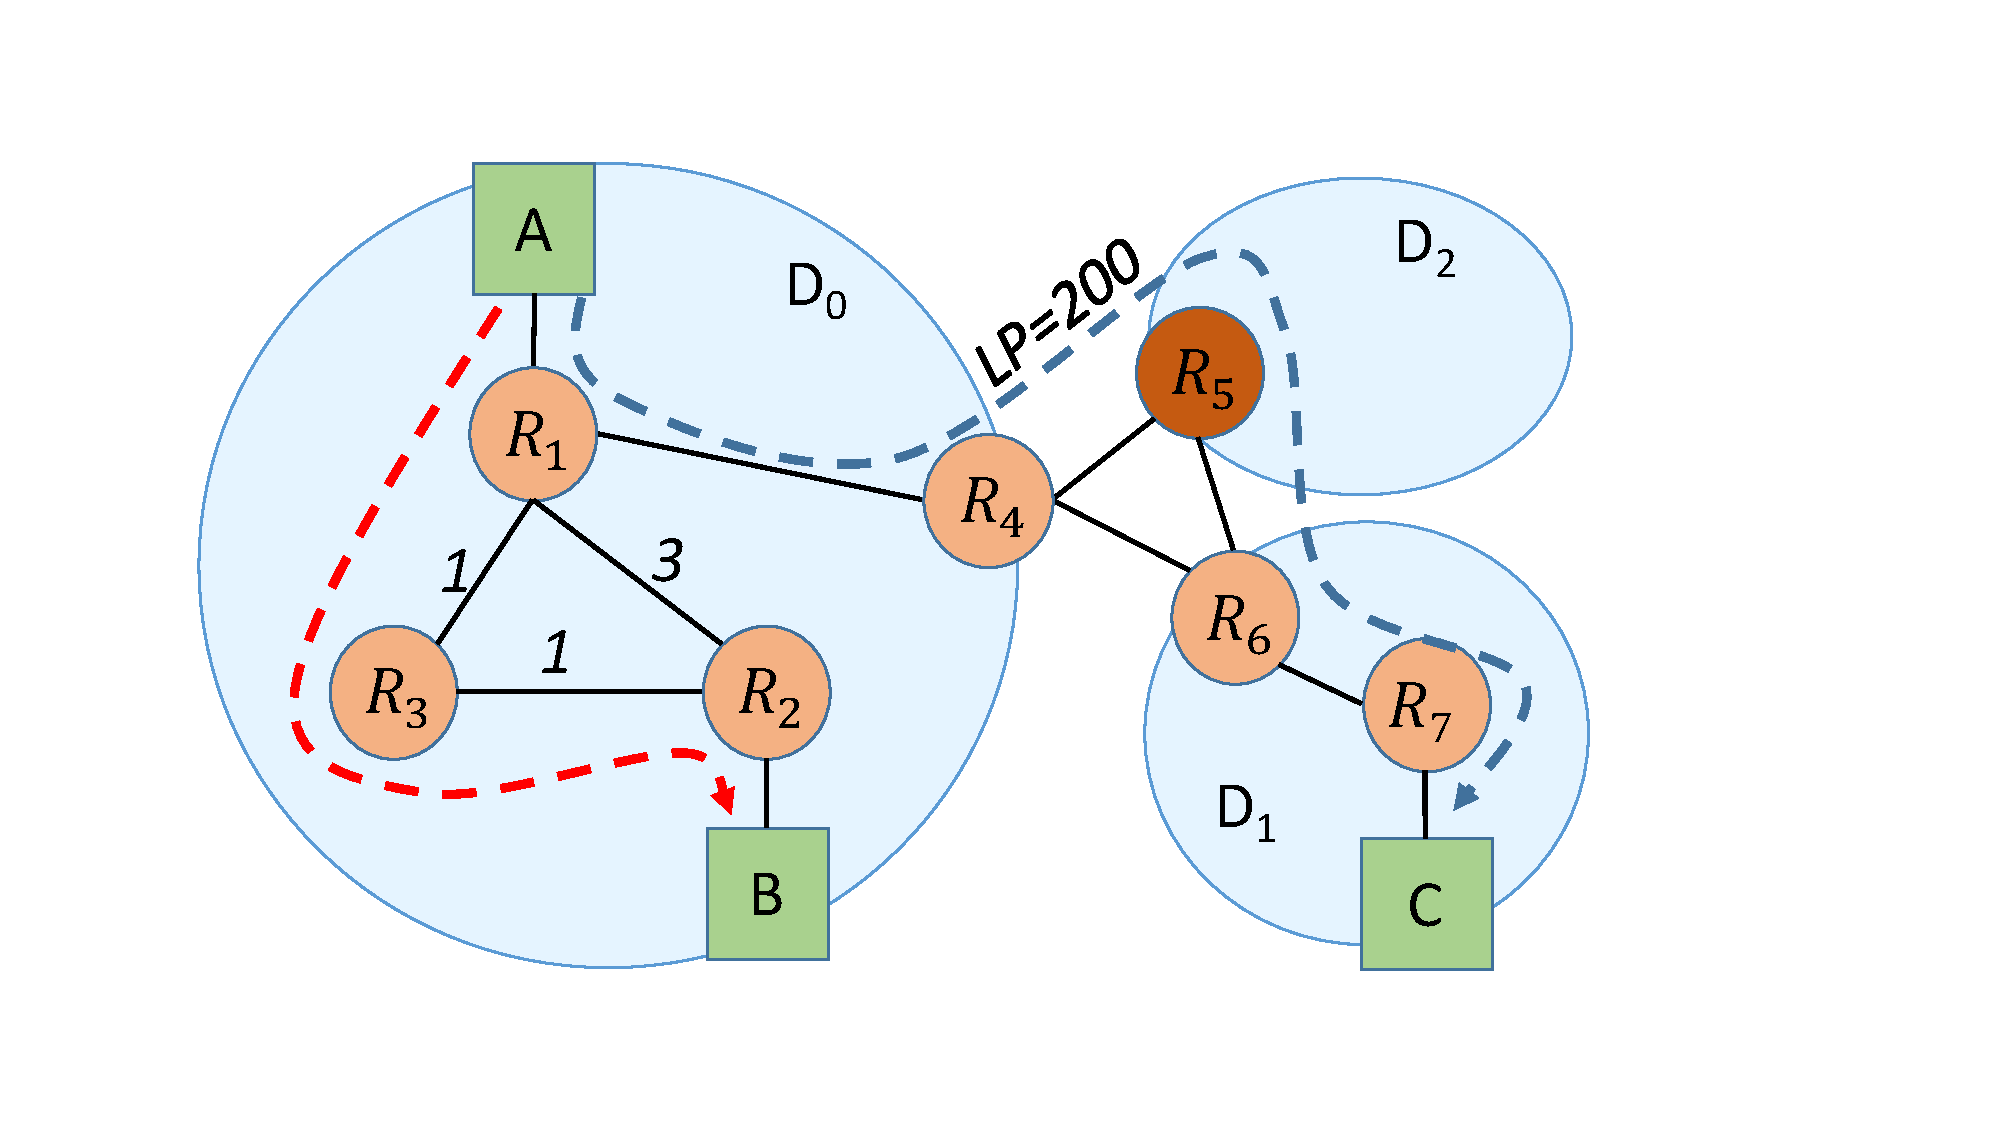
\includegraphics[width=0.75\columnwidth]{figures/example.pdf}
	\compactcaption{Example demonstrating the two-phase synthesis approach. 
	Genesis produces policy-compliant paths (red and blue), 
	which are used as input by Zeppelin to
	synthesize the OSPF and BGP configurations.}
	\label{fig:example}
\end{figure}

\begin{itemize}
	\item
For traffic $A \rightarrow B$, the path is entirely inside
a single OSPF domain, so Zeppelin has to find OSPF weights 
such that the shortest path is $R_1 \rightarrow R_3 \rightarrow 
R_2$. From the OSPF weights shown in \Cref{fig:example}, 
we can see that the weight of path $R_1 
\rightarrow R_3 \rightarrow R_2$ (2) is smaller than that of path
$R_1 \rightarrow R_2$ (5). 
 	\item For traffic $A \rightarrow C$, the path traverses through 
 	multiple domains, so Zeppelin configures BGP such that 
 	routing across domains follows the Genesis path. In this case, 
 	we need traffic to go through a longer path in terms of AS path
 	length; Zeppelin sets $R_4$'s BGP local preference for route C
 	from $R_5$ to a higher value (200), so that $R_5$ is 
 	preferred over $R_6$. 
 	\item Zeppelin can find better control planes in terms of how 
 	the network is split into domains. In this case,  
 	Zeppelin will suggest moving $R_5$ to domain $D_1$. 
 	This simplifies $R_4$'s BGP configuration as the local preference 
 	entry for C is not required. 
 	\item With a backup firewall at $R_8$, 
 	Zeppelin automatically synthesizes resilient OSPF configurations
          for $D_0$ such that if either $R_1-R_3$ or $R_3-R_2$ link
          fails, traffic to B goes through the firewall at $R_8$.
\end{itemize}

\section{Routing Model and Problem Definition}
In this section, we formally define the problem addressed in this
paper.  We first define common notations and then show how different
routing protocols are represented.  In particular, we model static
routes, OSPF shortest-path routing, and BGP preference-based routing.
Finally, we formally define when a certain configuration meets a given
set of policies and conclude with the configuration synthesis problems
we tackle.

\subsection{Routing Model}

\minisection{Preliminaries}
We represent the physical router topology as a directed graph $T=(V, L)$,
where $V$ is the set of routers and $L\subseteq V\times V$ is the set of links. 
Throughout the paper we assume $T$ is fixed.
We use the neighbour function $N(s) = \{s'\ | \ (s,s') \in L \}$ to denote 
the set of neighbour routers of $s$. 
We define $\Lambda$ to denote the set of destination IP subnets;
distributed protocols make forwarding decisions based on the 
destination address/subnet.

A path $\pi = (u_1,v_1) (u_2, v_2) \cdots (u_n, v_n) \in L^*$ is a loop-free valid path if
a  vertex is not visited more than once ($\forall i.j \leq n. 
~i \not= j \wedge u_i \not= u_j$) and adjacent links in the
path share a router ($\forall i < n. ~v_i = u_{i+1}$).
Sometimes we represent the path $\pi$ as $u_1\rightarrow u_2 \rightarrow  \cdots \rightarrow v_n$.
Given two nodes $s$ and $t$, we use $\Pi_s^t$ to denote the set of all paths
$\pi$ with source $s$ (i.e., $u_1=s$) and target $t$ (i.e., $v_n=t$). 
We also define the $\in$ operator for paths i.e., a link $l \in
\pi$ if $l$ is in the path. 

\name tackles the synthesis of a hierarchical control plane, 
where the network is divided into continuous domains. 
Each domain uses OSPF as the intra-domain routing protocol, 
and BGP for the inter-domain routing protocol. 
We define a router domain assignment function
$\Theta: V \rightarrow \nat$ which maps each router to a domain 
(denoted by a natural number).

The OSPF configurations are expressed 
using two functions: edge weights $W$ and
 route filters $RF$. For BGP configurations: 
we have the local preference function $LP$ 
and the iBGP filter function $IF$. Static 
routes are expressed using the $SR$ function.
We express the complete network configuration $C$
as a tuple $(\Theta,W,RF,LP,IF,SR)$.  In the 
rest of the section, we describe each component 
of the configuration $C$ and the routing function 
$\route^C$ for the network given $C$. We ensure one  
simplifying property for $C$: for two 
routers $r_1$ and $r_2$ in the network,
traffic will be forwarded from $r_1$ to $r_2$ 
along a single path. 
Thus, when synthesizing $C$, we ensure the components
of $C$ satisfy this property.


\minisection{Static Routes} Static routing refers to a router using a
manually-configured routing entry, rather than information from
dynamic protocols like OSPF or BGP.  It is useful to enforce certain
paths that are not easily realizable using routing protocols.  Static
routes have the highest preference over other routes for the same
destination at a router.  For a destination $\lambda$, a static route
configured at router $r$ ensures the traffic to forward to a
neighbouring router $r_1 \in N(r)$. We define the static route partial
function $SR: V \times \Lambda \mapsto V$ such that, for a router $r$
and destination $\lambda$, if $SR(r,\lambda)=r'$, then traffic for
destination $\lambda$ reaching node $r$ is always forwarded to node
$r'$. Using $SR$, we
construct the complete static paths between routers in the network
$\Pi_{SR}$. We assume $SR$ forms paths which replace OSPF or
BGP path fragments, \name will construct static routes based on this
property.

%These paths would have a highest preference.

\minisection{OSPF} Open Shortest Path First (OSPF) is a routing
protocol commonly used inside a domain. Each router receives link
state information from other routers and uses this to create a map of
the network. Positive weights are defined for each link in the
network, and each router used Djikstra's algorithm to forward to the
destination along the weighted shortest path to the router the
destination   is connected to.

Let us
define the OSPF weight function $W: L \rightarrow \rat$ which 
maps edges of the topology to positive rational weights. 
% todo: When to talk about converting LRA to LIA.
For a given
path $\pi=l_1\ldots l_n$, we indicate the sum of weights of the
links in the path by $W(\pi)=\sum W(l_i)$. 


We allow  route filters
to selectively disable an
edge for a given destination by  
blocking advertisements to a
particular destination along a link. 
Formally, a  route filter is a pair $(l,\lambda)\in L\times \Lambda$
which disables the link $l$ for destination $\lambda$. 
We define the  route filter function 
$RF: \Lambda \rightarrow 2^L$ which maps each destination  
to a set of filtered links in the topology. 
Given an   destination $\lambda\in \Lambda$, 
a legal path with respect to $RF$ and $\lambda$
is a valid path $\pi=l_1\cdots l_k$ such that for every $i$,
$l_i\not\in RF(\lambda)$.
We use $\Pi_\lambda$ to denote the set of all such paths.

We define the routing function 
$\route_{ospf}^G$ 
that given 
%a weight function $W$,
%a  route filter function $RF$,
a source node $s$,
a target node $t$,
and destination   
$\lambda$,
returns the OSPF-induced paths from $s$ to $t$ for destination   $\lambda$.
The paths between two nodes are
the shortest paths in the network
that do not cross any link that belongs to $RF(\lambda)$. We also
account for the higher priority of static routes.
\[
\route_{ospf}^C(s,t,\lambda) = 
\begin{cases}
\pi  & \text{$\Pi_s^t \cap \Pi_{SR} =\{\pi\}$} \\
\pi & 
\text{$\Pi_s^t \cap \Pi_{SR} =\emptyset \wedge \pi\in \Pi_s^t\cap \Pi_\lambda ~\wedge $}  \\
& \text{~~~~$\neg\exists \pi'\in\Pi_s^t\cap \Pi_\lambda . W(\pi')< W(\pi)$} 
\end{cases}
\]

\minisection{BGP} BGP is a path-vector inter-domain routing protocol
that connects different autonomous systems (ASes), where each AS
comprises of one or more routers (typically managed by a single
entity). A BGP router receives routes from BGP peers (internal peers
send iBGP routes, external peers send eBGP routes). Each route for the
destination comprises of a domain-level path to the destination
domain, and by default a BGP router will pick a path with fewest domains 
to forward the packet for a destination.
 
To support policy routing, BGP routers can be configured with a
\emph{local preference} variable to assign higher priorities to
specific routes for a particular destination. We define the local
preference function $LP: V \times V \times \Lambda \mapsto \nat$ as
follows.  Given a BGP router $r$, neighbouring router $r_1$, and  
destination $\lambda$, $LP(r, r_1, \lambda)$ specifies the local
preference for a route received for destination $\lambda$ at BGP
router $r$ from next-hop BGP router $r_1$.  This function is defined
on inter-domain links.  From the routes received at $r$, the router
picks the route with greatest local preference.

The Internal BGP (iBGP) protocol is used to 
exchange external BGP routes 
among BGP routers belonging
to the same domain. A external route received 
by $r_1$ with a local preference value configured 
will be advertised to the rest of the BGP routers of the 
domain as an iBGP route with the same local
preference. We can configure iBGP 
filters to prevent a router from advertising 
a route to another router. We do so using the 
function $IF: V \times \Lambda \mapsto 2^V$;
if a BGP router $r_1 \in IF(r_2, \lambda)$, then
$r_2$ will not advertise a route for $\lambda$ to
$r_1$ through iBGP. 
 
 \iffull
Algorithm~\ref{alg:bgppathrules} defines the routing function 
$\route_{bgp}^C$ 
that given 
%a local preference function $LP$,
a BGP router $r$
and destination  
$\lambda$,
returns 
the next-hop BGP router in the path. 
\else
We only describe the routing semantics of BGP
informally. The BGP path selection algorithm is submitted as part of the supplementary material.
\fi
BGP 
chooses a route with highest local preference, and
if there is a tie, it then chooses the route with smallest
AS path length~\cite{bgp}. 
\name synthesizes configurations where all ties are 
are broken using these criteria, and $\route_{bgp}^C(r,\lambda)$
returns a single router for the inter-domain next-hop router. 
Also, static routes 
have a higher preference than BGP, therefore a static route
$SR(r, \lambda)$ will be preferred over the BGP route.

\iffull
\begin{algorithm} [t]
	\begin{footnotesize} 
		\caption{BGP Best Path Selection at router $r$ for dst. $\lambda$}
		\label{alg:bgppathrules}
		\begin{algorithmic}[1]
			\Procedure{BestPath}{} \\
			\hspace*{0.4cm} [Each route $\gamma$ of form $(\lambda, local\_pref, len, nexthop)$]
			\State{$\Upsilon_{ebgp}$ = $\bigcup$ Route from external BGP neighbour for $\lambda$} 
			\State{$\Upsilon_{ibgp}$ = $\bigcup$ Route from internal BGP router $r_1$:
				 $r \not\in IF(r_1, \lambda)$}
			\State{$\Upsilon = \Upsilon_{ebgp}\cup \Upsilon_{ibgp}$}
			\\
			\If{$SR(r,\lambda) = r_1$} 
			\State{$\route^C_{bgp}(r, \lambda) = r_1$\hfill [Static Route has highest pref.]}
			\Else \\
			\indent\indent \hspace{0.3cm}[Find routes with highest \emph{local preference}]
			\State{$\Upsilon_{lp} = \{\gamma \in \Upsilon \mid \forall \gamma_1 \in \Upsilon. ~\gamma.local\_pref \geq \gamma_1.local\_pref\}$}
			\If{$|\Upsilon_{lp}| = 1$}
			\State{$\gamma_{best} = \gamma \in \Upsilon_{lp}$}
			\Else \newline
			\hspace*{0.7cm}\indent [Prefer the path with the smallest \emph{AS Path length}]
			\State{$\Upsilon_{as} = \{\gamma \in \Upsilon_{lp}  \mid \forall \gamma_1 \in \Upsilon_{lp}. ~\gamma.len \leq \gamma_1.len\} $}
			\If{$|\Upsilon_{as}| = 1$}
			\State{$\gamma_{best} = \gamma \in \Upsilon_{as}$}	
			\EndIf
			\EndIf
			\If{$\gamma_{best} \in \Upsilon_{ebgp}$}
			\State{$\route^C_{bgp}(r, \lambda) = \gamma_{best}.nexthop$}
			\State{Redistribute $\gamma_{best}$ to OSPF domain}
			\Else \\
			\hspace*{0.7cm}\indent [Traffic for $\lambda$ will not exit domain through $r$]
			\State{$\route^C_{bgp}(r, \lambda) = \bot$}
			\EndIf
			\EndIf
			\EndProcedure
			%				\State{ . }
			%				\State{Prefer the path with the lowest \emph{multi-exit discriminator} (MED).}
			%				\State{Prefer eBGP over iBGP paths.}
			%				\State{Prefer the route that comes from the BGP router with the lowest \emph{router ID}.}
		\end{algorithmic}
	\end{footnotesize}
\end{algorithm}
\fi

\minisection{OSPF+BGP+Static Routes} We now describe how routing
happens across domains.  In domain $d$, traffic 
for destination $\lambda$ originates at source
router $s$ (i.e., $\Theta(s) = d$). 
If the target router $t$ connected to the
destination belongs to domain $d$, then there exists a OSPF route for
$\lambda$ at $s$, and the path taken would be
$\route_{ospf}^C(s,t,\lambda)$.

Consider the case of destination $\lambda$ being connected 
to an external domain, thus, traffic for destination $\lambda$
will be sent to a BGP gateway router of domain $d$ which 
will forward it to its neighbouring domains till
it reaches the internal domain of $\lambda$. A BGP gateway
router is a router $g$ such that $\exists g' \in N(g). 
~\Theta(g') \not= \Theta(g)$. 

However, not all BGP routes for $\lambda$
are distributed 
into OSPF (to prevent explosion of forwarding tables). 
BGP gateways in a domain exchange routes using iBGP,
and if the best path chosen is an eBGP route, 
the gateway redistributes the eBGP route into OSPF. 
Therefore, multiple BGP routers
can redistribute a route for $\lambda$,  
the closest gateway (in terms of OSPF distance)
is chosen. We define a gateway function $G^C$,
that given a domain number $n\in \nat$
%a local preference $LP$,
%a weight function $W$,
%route filters $RF$,
a router $r$ such that $\Theta(r)=n$,
and destination $\lambda$ outside of domain $n$, 
specifies the
gateway chosen for a destination based on the
closest router redistributing the route for $\lambda$. 
Finally, the routing function 
$\route^C$
%:\Theta \times LP \times W \times RF \times V \times V \times \Lambda \rightarrow L^* 
returns paths from source to destination in a inter-domain network:
given a source $s_1$ and a destination $\lambda$ connected to target router $t$, 
\[
\begin{array}{c}
	\route^C(s_1, t, \lambda) = 
	\route_{ospf}^C(s_1,g_1, \lambda) + 
	 (g_1, s_2 )+\qquad\qquad\qquad  \\
%	~~~~~~~~~~~~~~~~~~~~~~~~~\route_{ospf}^C(s_2,g_2, \lambda) + (g_2, s_3) + \\
	\qquad\qquad\qquad\qquad \ldots  + (g_{n-1}, s_n) +\route_{ospf}^C(s_n,t,\lambda)
\end{array}
\]
Here, for each $i>1$, $g_i=G^C(\Theta(s_i),s_i,\lambda)$, 
$s_i=\route_{bgp}^C(g_{i-1}, \lambda)$,
and  $+$ is the concatenation operator for paths. 

\minisection{Induced paths}
We assume a set of packet classes $PC : [0,C_{pc}]$ 
and map each path (only reachability policies produce paths,
the rest specify properties on these paths)
to a unique integer in $PC$.
For a packet class $pc$, $src_{pc}$ denotes the source router,
$dst_{pc}$ denotes the destination router, and $\lambda_{pc}$
denotes the destination   address. 


\begin{definition}[Induced Paths]
Given a configuration $C$ and a set of packet classes $PC$, the set of paths
$\paths^C(PC)$ induced by $C$ is defined as follows: 
$\forall pc \in PC.$ $\route^C(src_{pc}, dst_{pc}, \lambda_{pc})$ $\in \paths^C(PC)$.
\end{definition}

\subsection{Problem Definition}
\begin{table}[!t]
\begin{small}
	\begin{center}
		\begin{tabular}{m{7.8em}  m{15.9em} } 
			{\bf Policy} & {\bf Description} \\ 
			\hline
			Reachability & There is a path from router $src$ to router $dst$ for destination $\lambda$ \\ \hline
			Reachability with \newline Ordered Waypoints & The path  from $src$ to $dst$ for destination $\lambda$ 
			traverses some switch in the set $W_1$, \ldots, then some switch in the set $W_k$.\\ \hline
			Traffic Isolation & Paths of two reachability policies $R1$ and $R2$ do not share  links \\ \hline
			Traffic Engineering  & Minimize total/max link utilization \\
		\end{tabular}
	\end{center}
	\compactcaption{\genesis path-based policy support.} \label{tab:policysupport} 
\end{small}
\end{table}


%\section{Policy Support} \label{sec:policy}
%We design a language GPL (Genesis Policy Language) for network operators to express the desired end-to-end policies in a declarative manner which is interpreted by the Genesis synthesizer to find the forwarding rules for the network topology which enforce the input policies (\cref{fig:arch}). Genesis supports the following policies : 
%% Figure of GPL's syntax
%\begin{enumerate} 
%	\item \textbf{Reachability}: $predicate : src >> dst$ \\
%	This policy specifies the packets satisying $predicate$ have ingress router $src$ and egress router $dst$, and requires rules forwarding packets satisfying $predicate$ from $src$ to $dst$. There must be no forwarding loops in the network. 
%	\item \textbf{Waypoint}: $predicate : src >> W >> dst$ \\
%	The waypoint policy is a stronger reachability policy, and specifies that packet satisfying $predicate$ with ingress router $src$ and egress router $dst$ must pass through the set of waypoints $W$ in no particular order. The waypoint policy helps operators and tenants to specify the middleboxes the packets must traverse through without worrying about order, or having to use header tags to enforce a particular order \cite{flowtags}. 
%	\item \textbf{Traffic Isolation}:  $R1 \ || \ R2$ \\
%	The traffic isolation policy ensures that the . This policy can be used to provide fairness guarantees, since the paths of $R1$ and $R2$ don't share a link, the bandwidth used by $R1$ will not affect the bandwidth used by $R2$ and vice-versa. The condition of sharing a link in the same direction is due to the fact that links are full-duplex so, traffic flowing in one direction is not affected by the traffic flowing in the other direction.
%	\item \textbf{Security Isolation}: $R1 <> R2$ \\
%	The security isolation policy is stronger than the traffic isolation policy, and ensures that the path of the reachabiltiy/waypoint policies $R1$ and $R2$ do not share a link in both directions for increased security.
%	\item \textbf{}: $sw_1 \rightarrow sw_2 : capacity$ \\
%	The link capacity policy specifies that the capacity for link $sw_1 \rightarrow sw_2$ is $capacity$, and the weights of flows traversing the link in the direction of $sw_2$ do not exceed the capacity of the link.  
%	\item \textbf{Switch Table Size}: $sw : size$ \\
%	The router table size policy is used to specify the size of the forwarding table of the router $sw$ and ensures that the number of flows traversing through $sw$ does not exceed $size$ as each flow would require a forwarding rule at the switch.
%\end{enumerate}

\begin{table}[t!]
\begin{small}
	\begin{center}
		\begin{tabular}{m{7em} | m{17em} } 
			Policy & Description \\ 
			\hline
			Count & Number of continous OSPF domains  \\ \hline
			Domain Size  & Lower and upper
			limit of size of domain (number of routers) \\ \hline
			BGP \newline Disable & Disable BGP on router (hardware constraint). 
			Router cannot lie on boundary of domain \\ \hline
			Endpoint \newline Resilience: $rc$ & Lower bound endpoint resilience: \newline
			$rc > C_{rc}$\\ \hline
			Static Route: ${sc}$ & Upper bound number of static route rules: $sc < C_{sc}$ \\ \hline
			BGP Config. Overhead: $bc$ & Upper bound the number of local preference entries and iBGP filters $bc < C_{bc}$ \\ \hline
			Cost Minization & Minimize user-defined cost $expr(rc, sc, bc)$
		\end{tabular}
	\end{center}
	\compactcaption{\name Domain assignment policy support.} \label{tab:configpolicysupport} 
\end{small}
\end{table}


\minisection{Policies}
\Cref{tab:policysupport} describes the path policies supported by \name.
Given  a set $\Psi$ of
path policies, we say that
a set of paths $\Pi$ is policy-compliant with respect to $\Psi$, $\Pi \models \Psi$,
if the paths in $\Pi$ satisfy all the policies in $\Psi$ (see~\cite{genesis} for the formal definition). 


\Cref{tab:configpolicysupport} describes all the configuration policies supported by \name.
A configuration $C$ satisfies a set of configuration policies $P$
if $C$ satisfies every constraint in $P$.
For each configuration policy 
we define what it means for  a configuration $C=(\Theta,W,RF,LP,IF,SR)$ to satisfy it.

The first type of policy restricts how many OSPF domains $N_D$ a
configuration might have, $c_1\leq N_D\leq c_2$ 
and it is satisfied by $C$ iff $c_1\leq |\{\Theta(r)\mid r\in V\}|\leq
c_2$.  This policy is useful for avoiding situations resulting in too
many domains in the hierarchical split which can be difficult to
administer.  The second type of policy allows the operator to restrict
the size $k$ of each OSPF domain, $l\leq k\leq u$, because OSPF does
not scale gracefully with network size.  This policy is satisfied if
for every domain $i$, $l\leq |\{r \mid \Theta(r)=i\}|\leq u$.


Certain 
	routers may not be suited to run BGP due to resource
	constraints. Thus, the operator can specify what set of 
	routers $B\subseteq V$ is BGP compatible.  
	This policy is satisfied if none of the routers $V\setminus B$
	is a gateway router.
	Formally, for every $r\in V\setminus B$,
	there doesn't exist a router $r'\in N(r)$ such that $\Theta(r) \not= \Theta(r_1)$

Finally, \name provides ways to specify upper bounds on the number of
1) route filters, which in general reduce the resiliency of the network---i.e., $rc=|\cup_{\lambda\in \Lambda} RF(\lambda)|\leq C_{rc}$,
2) static routes---i.e., $sc=|\{(v,\lambda)\mid \exists v'. SR(v,\lambda)=v'\}|\leq C_{sc}$, and
3) BGP configurations, which increase the complexity of the network---i.e., 
$bc=|\cup_{v,\lambda\in V\times\Lambda} IF(v,\lambda)\cup \{(v,v',\lambda)\mid LP(v,v',\lambda)\neq \bot|\leq C_{bc}$.
\name also allows to minimize certain expressions over the quantities $rc$, $sc$, and $bc$---e.g., $max(rc, sc+bc)$. 
Ideally, the most important metric we want to maximize is resiliency---i.e.,
the number of alternate paths between endpoints.
However, this metric is too hard to handle as it depends on complex graph properties. 
In practice, when we want improve resiliency, we try to minimize
the number of filters; we will show that this strategy is effective. 

%different configuration metrics. For example,
%we allow  route filters in OSPF synthesis 
%(\secref{sec:ospfsynthesis}), which may yield undesirable
%endpoint resilience, thereby, synthesizing configurations
%which provide a specified metric of resilience or maximize
%the metric. Similarily, to enable path-based inter-domain routing, 
%\name needs	to set up static routes along the path, or configure BGP 
%variables like local preferences to ensure the configurations 
%induce the input paths.
%These increase the size of the configurations,
%thus increasing the complexity of verifying correctness either 
%manually or using verification tools~\cite{batfish, arc, era}. 
%Therefore,
%another objective \name considers is the configuration overhead
%to ensure path-compliance.



\minisection{Synthesis problems}
\noindent We can now define what it means for a configuration $C$ to be policy-compliant
and our synthesis problems.
\begin{definition}[Policy-Compliance] \label{def:policycompliance}
	Given a set of path policies $\Psi$ and a set of configuration policies $P$,
	the configuration $C$ is policy-compliant with $(\Psi,P)$,
	$C \models (\Psi,P)$, if the set of
	induced paths $\paths^C(PC) \models \Psi$
	and $C$ satisfies the policies in $P$.
	The \emph{configuration synthesis problem} is to find, given $\Psi$ and $P$,
a configuration $C$ that is policy compliant with $(\Psi,P)$.
\end{definition}

As anticipated in Section~\ref{sec:motivation}, our approach will proceed in two phases,
one of which solves the following sub-problem.  
\begin{definition}[Path-Compliance] \label{def:pathcompliance}
Given a set of configuration policies $P$,
and a set of paths $\Pi$ over packet classes $PC$,
	a configurations $C$ is path-compliant with 
	$(\Pi,P)$,
	if $\paths^C(PC)=\Pi$ and $C$ satisfies the policies in $P$.
	The \emph{path-compliance synthesis problem} is to find, given $P$ and $\Pi$,
a configuration $C$ that is path-compliant with $(\Pi,P)$.
\end{definition}




%We defined policy-compliance in terms of the 
%paths of the packet classes satisfying path-based 
%policies like isolation or traffic engineering. However,
%depending on the assignment of routers to different domains,
%the configurations generated may not be efficient
%in deployment. Therefore, we extend the notion of 
%compliance to policies on configurations 
%(\Cref{tab:configpolicysupport}).



%\section{From Policies to Paths} \label{sec:genesis}
Directly generating policy-compliant configurations is a challenging
problem.
Therefore, all the techniques we present in this paper 
use a two-phased approach in which we first synthesize
policy-compliant \emph{paths} using the tool \genesis~\cite{genesis}
and then use the synthesized paths as \emph{hints} to synthesize resilient configurations. 
In this section, we recall the features of \genesis,
 a tool for generating policy-compliant paths, and describe
some modifications that are necessary to generate paths that
can be realized by routing protocols. 

%that result in the paths we
%synthesized in the first phase; we refer to tool that performs the second phase as \name.
%The first phase may produce \emph{bad} paths for which the
%configuration synthesis is complicated or not possible. Thus, we
%propose ways to restart the algorithm by computing new paths.

%\subsection{\genesis: From Policies to Paths} \label{sec:genesis}
\genesis is a network management
system which synthesizes forwarding tables enforcing some input policies. 
Some of the policies supported by \genesis are specified in 
\Cref{tab:policysupport}. 
%Due to the rich policy language, generating policy-compliant paths is an NP-complete problem;
%\genesis mitigates this problem by leveraging the power of SMT solvers.
% to provide
%support for policy enforcement for a diverse set of policies.
Given a set of policies, \genesis generates a set of constraints 
so that solutions to these constraints are forwarding
tables that can be used to extract the 
policy-compliant paths.
The generated constrains are over the relation $Fwd \subseteq V \times V \times PC$,
which captures
the network forwarding behavior---i.e. 
$(r_1, r_2$, $pc)\in$ $Fwd$ if 
$r_1$ forwards packets of class $pc$ to router $r_2$---
and 
the relation $Reach \subseteq V \times PC \times \nat$,
which captures
reachability---i.e. $(r, pc, k)\in Reach$ if 
the router $r$ is reachable in the path from the source
router of packet class $pc$ in exactly $k$ steps.
% Based on
%the input policies, \genesis generates constraints over the $Fwd$
%and $Reach$ relations. Finally, \genesis uses the solution to the relations to extracts the concrete paths.

\paragraph{Modifications to \genesis}
OpenFlow switches~\cite{openflow} support predicates for
forwarding rules on different packet header fields such as source
and/or destination IP address, ports etc. However, legacy protocols
like OSPF and BGP only support destination-based forwarding, 
forcing the paths to a destination subnet to 
form a directed tree rooted at the destination. 
Thus,
at any router, there exists at most one forwarding rule per destination. 
Since \genesis was built for
SDN management,  a switch may forward to different switches
packets that are directed to the same destination;
this behaviour cannot be induced with router
configurations. We  discuss how the
constraints of \genesis
need to be modified to avoid generating paths that 
cannot be enforced using routing configurations.

Concretely, we modify the constraints given to \genesis to ensure that,
if any two paths to a destination subnet intersect at a router,
the subsequent downstream paths from the router to the destination 
 do not \emph{diverge} at another router.  
We define the relation $Reach^*(r,pc)$ to model reachability 
of $r$ in the path of $pc$---i.e., $r$ is traversed by the path for packet class $pc$. 
If we allow paths of length at most $\mu$, we can define $Reach^*(r,pc)$ as:
\begin{equation}
	Reach^*(r,pc) \Leftrightarrow \bigvee_{k \in [0, \mu]} Reach(r, pc, k).
\end{equation}
To guarantee that the generate paths can be enforced using destination-based
forwarding we add
the following constraint for every pair of packet classes $pc_1$ and $pc_2$ that belong to the same 
 destination subnet:
 \begin{equation}
 \forall r. Reach^*(r, pc_1) \wedge Reach^*(r, pc_2) 
 \implies \\ \bigwedge_{n \in N(r)} Fwd(r, n, pc_1) \Leftrightarrow Fwd(r, n, pc_2)
 \end{equation}
Intuitively, 
 if a router $r$ is reachable for both packet classes, 
the next router $n$ in the path must be the same for both classes. Thus, the paths obtained
 from \genesis for a destination will form a 
 directed destination tree.
 We will use this property in Section~\ref{sec:intra-synthesis}. 

%\subsection{\name: From Paths to Router Configurations} 
%After we have computed a set of policy-compliant paths,
%we need to solve the path-compliance problem using such paths.
%To solve this problem \name
%combines techniques in constraint solving and randomized search
%to efficiently generate router configurations for the paths obtained from \genesis.
%For a given domain division of the network,
%\name uses linear constraints to generate OSPF weights and 
%the structure of the paths  to generate BGP preferences.
%If the generated linear  constraints cannot be solved, \name uses the unsatisfiable cores to
%identify where to place route filters.
%To decide how to split the network into domains,
%\name uses Markov Chain Monte Carlo (MCMC) search to find
%domain assignments that satisfy the configuration policies and have good resilience.
%When the MCMC search does not progress and cannot find good solutions,
%we restart the search by asking \genesis to generate a new set of paths that is different from
%the previously generated ones.
%These techniques are described in detail in the next two sections.

%\subsection{Challenges}
%\minisection{OSPF Synthesis}
%For the OSPF protocol, configurations assign
%weights to links between routers (directed edges
%in the network topology). When the network has
%to forward a packet from $s$ to $t$, the
%OSPF routers uses 
%Djikstra's algorithm to chose the
%shortest weighted path from $s$ to $t$. Thus,
%given input paths, \name finds edge weights 
%(which are global for all paths) such that 
%the shortest path through the network
%for these endpoints exactly match the input paths. 
%For example in \Cref{fig:ospfexample}(a), if the input
%path is $s\rightarrow r_1 \rightarrow t$ for
%destination IP $\lambda$, \name assigns
%edge weights such that the input path has a strictly
%smaller weight ($w=1+2$) than the other path $s \rightarrow t$ 
%($w=5$). Thus, the OSPF routers will forward traffic for
%$\lambda$ from $s$ to $t$ through $r_1$. \name 
%efficiently computes weights by generating constraints
%in the theory of Linear rational arithmetic (LRA) and
%uses fast off-the-shelf LP Solvers 
%(\secref{sec:ospfsynthesis}). 
%
%However, given a set of paths as input, there may
%not exist a solution to the edge weights. Consider the 
%input paths as shown in \Cref{fig:ospfexample}(b). 
%Both the red and blue paths are required 
%to be the unique shortest path between $s$ to $t$
%and, clearly, this is cannot be enforced for any 
%choice of the edge weights (as weights correspond 
%to all destinations). 
%One way to synthesize configurations in this scenario 
%is to ``disable'' the edge
%$(s, t)$ for destination $\lambda_1$.
%Using this technique, 
%there is only one possible path from $s$ to $t$
%for destination $\lambda_1$ ($s\rightarrow r_1 \rightarrow t$),
%therefore is chosen as the shortest path. For 
%destination $\lambda_2$, the $s\rightarrow t$ path
%has a smaller weight ($w=1$) than the
%$s\rightarrow r_1 \rightarrow t$ path ($w=1+2$), therefore,
%both traffic is forwarded through the input paths for
%both the destinations. 
%This blocking mechanism is called a route filter, and
%we modify \name's OSPF synthesis algorithm to support
%route filtering (\secref{sec:filtering}).
%
%
%\begin{figure}
%	\centering
%	\subfloat[Edge Weights]{
%		\raisebox{0.5cm}{\resizebox {0.5\columnwidth} {!} {
%				\begin{tikzpicture}[shorten >=0.5pt,node distance=,on grid,auto,
%				square/.style={regular polygon,regular polygon sides=4}] 
%				\node[state] at (0,0) (s)  {$s$}; 
%				\node[state] at (1.8,1) (v1)  {$r_1$}; 
%				\node[state] at (3.6, 0)(t) {$t$};
%				\node[state, rectangle] at (5, 0) (d1) {$\lambda$};
%				\path[->] 
%				(s) edge node {1} (v1)
%				edge  node {5} (t)
%				edge [red, dashed, bend left=90] node {} (t)
%				(v1) edge node {2} (t)
%				(t) edge [red, dashed] node {} (d1);
%				\end{tikzpicture}
%			}}}
%			\subfloat[Route Filters]{
%				\resizebox {0.5\columnwidth} {!} {
%					\begin{tikzpicture}[shorten >=0.5pt,node distance=,on grid,auto,
%					square/.style={regular polygon,regular polygon sides=4}] 
%					\node[state] at (0,0) (s)  {$s$}; 
%					\node[state] at (2, 1) (v1)  {$r_1$}; 
%					\node[state] at (4, 0)(t) {$t$};
%					\node[state, rectangle] at (5.5, 0.75) (d1) {$\lambda_1$};
%					\node[state, rectangle] at (5.5, -0.75) (d2) {$\lambda_2$};
%					\path[->] 
%					(s) edge node {1} (v1)
%					edge  node [above] {1} node [below] {$rf((s,t),\lambda_1)$} (t)
%					edge [red, dashed, bend left=90] node {} (t)
%					edge [blue, dashed, bend right=45] node {} (t)
%					(v1) edge node {2} (t)
%					(t) edge [red, dashed] node {} (d1)
%					(t) edge [blue, dashed] node {} (d2);
%					\end{tikzpicture}
%				}}
%				\compactcaption{OSPF edge weights and filters such that the
%					the routers forward traffic for destination along
%					the input paths (dashed arcs).}
%				\label{fig:ospfexample}
%			\end{figure}
%			
%			
%			
%\minisection{Dynamic Domain assignment}
%The OSPF routing protocol does not scale 
%with increasing network sizes
%as it uses reliable
%flooding of link-state packets. Flooding 
%of updates can  
%overwhelm the network when links fail. 
%Ideally, operators would want to specify
%limits on the size of an OSPF routing domain. 
%Thus, a network could be 
%split into multiple continuous OSPF domains,
%which exchange routes across domains using
%a inter-domain protocol like BGP.
%
%We augment \name to synthesize 
%inter-domain routing configurations 
%such that each router is assigned to
%a particular domain. 
%Each domain is continous (all routers
%are reachable to one another) and 
%uses OSPF for intra-domain routing.
%Domains exchange routes among  
%themselves using BGP, a path-vector 
%protocol which primarily selects routes by 
%the number of domains in the route. 
%However, \name can 
%use BGP's powerful path selection metrics 
%like local preferences such that  
%paths with greater path lengths are selected.
%OSPF has better convergence times than BGP,
%thus, it is advantageous to use OSPF for 
%routing in small domains and using BGP for
%inter-domain routing. 
%
%We consider the network to be managed by a 
%single entity, therefore, the network can 
%be split into domains\footnote{
%	The Internet is split into domains depending 
%	on ownership.} in numerous ways. Depending
%on the network and input data plane, a certain
%domain assignment of routers 
%can optimize different metrics, like the
%inter-domain configuration overhead (like BGP local
%preferences and static routes) and OSPF route filters
%in the different domains. Thus, instead of operators
%specifying a static domain assignment, \name stochastically
%searches for the best domain assignment from the space of 
%allowed assignments (for e.g., adhering to domain size limits)
%to optimize different metrics. \name uses 
%\emph{Markov chain Monte Carlo} sampling (MCMC) to perform
%this stochastic search, and operators can specify parameters
%to tune the cost function used in the search to assign priorities
%to different metrics. 

%!TEX root = paper.tex
\section{From Policies to Connectivity-Resilient \\ Configurations}
\label{sec:config-synthesis}

We now present an algorithm
for synthesizing distributed configurations
that adhere to path policies like the one described 
in Figure~\ref{tab:policysupport}.
In general, no existing tool for synthesizing 
distributed configurations
can handle this heterogeneous set of 
these policies---e.g., isolation---and, even less so,
generate resilient configurations.
Due to the complexity of the problem, we focus on 
synthesizing  configurations that 
are \emph{policy-compliant} and have high \emph{connectivity-resilience}.



\subsection{A two-phase approach}
Existing approaches to configuration synthesis
try to directly generate configurations from the given policies~\cite{synet},
but a direct approach leads to scalability issues as well as limitation
in the set of supported policies.
Instead of directly generating configurations from policies, 
\name uses a two-phase approach:
first it generates policy-compliant paths
and then it synthesizes distributed configurations that realize these paths
and have high connectivity resilience.

For the first phase, we use \genesis~\cite{genesis}, 
a network management system which synthesizes 
SDN forwarding tables enforcing some input policies. 
Some of the policies supported by \genesis are specified in 
\Cref{tab:policysupport}. 
Given a set of policies, \genesis generates a set of constraints 
so that solutions to these constraints are forwarding
tables that can be used to extract the 
policy-compliant paths. 

However, we need to modify the \genesis constraints
to integrate with \name. Legacy protocols only
support destination-based forwarding, unlike OpenFlow switches~\cite{openflow}. 
A router cannot forward a subnet's traffic 
to different routers based on source (or other 
packet headers). Thus, we add additional constraints to ensure
the paths generated by \genesis follow destination-based 
forwarding: paths obtained from 
\genesis for a destination will form a directed tree. 

Let us now look at how we solve the path-compliance problem.
Formally, we are given a set of paths $\Pi$,
a topology $T=(V,L)$,
a domain-assignment function $\Theta$, 
%and configuration policies $P$,
and we want to find functions of the configuration
$C=(\Theta,W,LP,IF,SR)$ such that
$\paths^C(PC) = \Pi$.
%., and
%$C$ satisfies $P$.
%Ideally, we want to directly generate configurations that maximize 
%connectivity resilience, but already generating policy-compliant configuration is
%a hard problem.
\kausik{In a software-defined OpenFlow~\cite{openflow} network, 
we can program
switch rules to forward traffic 
to a particular next-hop switch. 
Therefore, a trivial solution to the path-compliance problem 
in SDNs is to install forwarding rules along the policy-compliant
paths~\cite{genesis}. Static routes provide the functionality
of specifying the next-hop router,
thus, a solution to the path-compliance problem is to simply
add a static route to $SR(\lambda)$ for every link $l$ in 
set of the paths $\Pi$. Similar to static routes,
Fibbing~\cite{fibbing} used fake 
advertisements to achieve fine-grained control over
OSPF forwarding.}

\kausik{
Under no failures, the trivial 
solution of using static routes ensures 
policy-compliance, as traffic follows the paths provided by \genesis. 
However, this solution uses more static routes than necessary
and, in the presence of failures, static routes may
create routing loops that make certain connections 
unreachable, hence reducing connectivity-resilience.
Thus, we set our goal to synthesizing configurations
which are policy-compliant when there are no network 
failures, and improving connectivity-resilience by using
fewer static routes.}


% In the following sections, we assume we are given paths that are compliant to 
% all path policies and we only need to find configurations that realize those paths.
% Therefore, the algorithms we present solve the path-compliance synthesis problem
% and whenever we discuss soundness and completeness is with respect to such a problem.
% In general, for a given set of paths, we might not be able to find a path-compliant configuration
% that satisfies all the required configuration policies. However, in this case
% we can simply use ~\genesis to generate a different set of paths.
% Assuming we have a sound and complete algorithm for the
% path-compliance synthesis problem, we can obtain a sound and complete algorithm
% for the
%  configuration synthesis problem by keeping enumerating more policy compliant paths
%  whenever the path-compliance synthesis fails.

We first show how to synthesize 
path-compliant intra-domain 
configurations and then extend to
 inter-domain configurations.



\subsection{Synthesizing Path-compliant Intra-domain \\ Configurations} \label{sec:intra-synthesis}
% To justify the complexity of the techniques 
% we are going to present,
% we show that
% %, even when policy-compliant paths are provided, 
% obtaining configurations with minimal numbers of static routes is a 
% computationally hard problem.

\iffull
\begin{theorem}[Hardness of synthesis]
\label{thm:ospfsynth}
Given a
network with a single domain,
and a positive number $C_{sc}$,
the problem of generating
a path-compliant configuration with at most $C_{sc}$ static routes
is NP-complete.
\end{theorem}
%!TEX root = paper.tex
\begin{proof}
We show that the decision version of the minimum 
vertex cover problem, i.e., there exists a vertex cover
of size $ \leq k$, which is NP-complete, 
reduces to finding a set of static routes 
of size $ \leq k$ \
and OSPF weights for a network with only one domain. 
The latter is also in NP, so after the reduction we 
can conclude that it is also NP-complete.

Let $G = (V,E)$ be an instance of the 
minimum vertex cover problem. A set of
vertices $VC \subseteq V$ is the vertex cover
if $\forall (v_1, v_2) \in E. ~v_1 \in VC \vee v_2 \in VC$. 

We now show how to construct a topology $T=(S,L)$ 
and a corresponding set of paths $\Pi$ that can be enforced 
by configuration C which requires static routes $SR$ such that $|SR| \leq k$  
if and only if the corresponding $VC(SR)$ is a vertex cover of 
the graph $G$ and $|VC(SR)| \leq k$.

\paragraph{Construction.}
For every vertex $v \in V$: add a vertex $r_v$.
For every edge $(u,v) \in E$: add two vertices $s_{uv}$
and $t_{uv}$ to $S$. Add edges
connecting $s_{uv} \rightarrow r_{u}$, $s_{uv} \rightarrow r_{v}$,
$r_{u} \rightarrow t_{uv}$ and $r_{v} \rightarrow t_{uv}$. 
\Cref{fig:rfcomplexity} illustrates this construction.
\begin{figure}[H]
	\centering
	\begin{tikzpicture}[shorten >=0.5pt,node distance=1.5cm,on grid,auto,
	square/.style={regular polygon,regular polygon sides=4}] 
	\node[state] at (0,0) (s)  {$s_{uv}$}; 
	\node[state] at (3,-1) (v)  {$r_v$}; 
	\node[state] at (3,1) (u)  {$r_u$}; 
	\node[state] at (6,0) (t) {$t_{uv}$}; 	
	\node[state] (s1) [below=of s] {$s_{vw}$}; 	
	\node[state] (t1) [below=of t] {$t_{vw}$}; 	
	\path[-] 
	(s) edge  node {} (v)
	edge  node {} (u)
	edge [blue, dashed, bend right=40] node {} (t)
	edge [red, dashed, bend left=40] node {} (t)
	(u) edge node {} (t)
	(v) edge node {} (t)
	edge node {} (t1)
	edge node {} (s1);
	\path[->]
	(s)
	edge [blue, dashed, bend right=40] node {} (t)
	edge [red, dashed, bend left=40] node {} (t);
%	\path[-] (s) edge node[above] {} +(1,-0.1);
%	\path[-] (t1) edge node[above] {} +(-1,-0.1);
	\end{tikzpicture}
	\caption{Construction for reduction to Vertex Cover.}
	\label{fig:rfcomplexity}
\end{figure}
If there is another edge $(v,w) \in E$, then
$s_{vw}$ and $t_{vw}$ have an edge connecting to $r_v$ (shown
in \Cref{fig:rfcomplexity}). 

For each edge $(u,v) \in E$, we add two paths in $\Pi$: 
$s_{uv} \rightarrow r_u \rightarrow t_{uv}$
for destination host $d_u$ and 
$~s_{uv} \rightarrow r_v \rightarrow t_{uv}$ 
for destination host $d_v$.
(dashed paths in \Cref{fig:rfcomplexity}). 

We now prove that if there exists a set of static routes
$SR$ such that $|SR| \leq k$ such that the resulting configurations
are path-compliant for $\Pi$, then there exists a vertex cover $VC$
of $G$ such that $|VC| \leq k$. 

For each static route $sr \in SR$, the static route
has to be placed at the source, either going to $r_u$
or $r_v$ (structure of topology $T$). 
We construct a set $VC(SR)$ by adding the vertex $v$
based on the endpoints of each static route $sr \in SR$.
To show that $VC(SR)$ is a vertex cover of $G$, we first
prove \Cref{lemma:diamond}.

\begin{lemma} \label{lemma:diamond}
	 For each diamond formed by the input paths, atleast 1 
	 static route on one of the edges of the paths of the diamond 
	 is required to find a valid solution to the
	 OSPF edge weights.  
\end{lemma}

\begin{proof}
Given two paths $\pi_1$ and $\pi_2$ for destinations 
$d_u$ and $d_v$, we define these paths form a diamond
if these paths intersect at two routers ($s_{uv}$ and $t_{uv}$) 
without any common router in between. 
Consider the following diamond % in \Cref{fig:diamond}
constructed by paths $\pi_1$: $s_{uv} \rightarrow r_u \rightarrow t_{uv}$ 
for destination $d_u$ and $\pi_2$: $s_{uv} \rightarrow r_v \rightarrow t_{uv}$ 
for destination $d_v$. Let us assume there exists a solution 
for the OSPF edge weights without any static routes. 

We add the following inequality 
to make $\pi_1$ is the shortest 
path from $s_{uv}$ to $t_{uv}$ by
ensuring
 $\pi_1$ is shorter than the
path from $s_{uv}$ to $t_{uv}$ via $r_v$: 
\begin{equation} \label{eq:diamond1}
	W(s_{uv},r_u) + W(r_u, t_{uv}) < W(s_{uv}, r_v) + W(r_v,t_{uv})
\end{equation}
Since $\pi_2$ is also the shortest path from $s_{uv}$ 
to $t_{uv}$, the linear inequality added is:
\begin{equation}  \label{eq:diamond2}
W(s_{uv},r_v) + W(r_v, t) < W(s_{uv}, r_u) + W(r_u,t_{uv})
\end{equation}
Since there are no static routes on the edges
of $\pi_1$ and $\pi_2$, none of the above equations are 
eliminated. 
Adding equations \ref{eq:diamond1} and  \ref{eq:diamond2} 
yields the inequality $0 < 0$, which is inconsistent 
and therefore, no solution to 
the edge weights exists for this system of equations, 
which contradicts our assumption. Therefore,
for each diamond formed by the input paths, atleast 1 
static route on one of the edges of the paths of the diamond 
is required to find a valid solution to the
OSPF edge weights.  
\end{proof}

For every edge $(u,v) \in E$, the constructed paths from 
$s_{uv}$ to $t_{uv}$ form a diamond. Thus, by Lemma~\ref{lemma:diamond}, 
the diamond created by the paths corresponding to each edge in $G$ 
requires atleast one static route to eliminate
the inconsistency caused by the diamond. If a static route's endpoints
contains $r_u$, we put $u$ in $VC(SR)$ and similarily for $r_v$. 
Edge $(u,v)$ is covered since atleast one static route is added,
thus, atleast one of $\{u,v\}$ is in $VC(SR)$.  
Thus, if $SR$ eliminates all diamond inconsistencies
to find a solution to the OSPF weights, the corresponding set
$VC(SR)$ covers all edges in $E$. Therefore, $VC(SR)$ is a vertex
cover. 

Thus, by finding a set of static routes $SR$ such that $|SR| \leq k$
such that all the diamond inconsistencies are eliminated, and there
exists OSPF weights $W$ such that the configurations forward traffic
along $\Pi$, we can find a vertex cover $VC$ for graph $G$ such that
$|VC| \leq k$. 

This transformation is polynomial, the constructed 
network topology $T$ has $|V| + 2|E|$ nodes, 
$4|E|$ links and $2|E|$ paths. Therefore, OSPF
configuration synthesis with number of static routes $\leq k$ is
NP-complete. Thus, OSPF synthesis with minimal number of 
static routes is NP-hard. 
\end{proof}

%\else
%The reduction is from the vertex cover problem.
\fi

In this section, we show how to synthesize 
path-compliant  intra-domain configurations that
use few static routes.
The problem of optimally placing 
static routes is NP-hard (Theorem~\ref{thm:ospfsynth}), 
therefore, we propose a non-optimal greedy strategy.
We first show how to solve the problem when 
there exists a solution with no static routes
and then extend our technique to greedily 
add static routes when needed. We use 
efficient off-the-shelf linear programming 
solvers for solving the system of constraints 
which are presented in the following sections. 
	

\subsubsection{Intra-domain Synthesis without Static Routes} \label{sec:ospf}\hspace*{4mm}


 
In the absence of static routes,
OSPF routers use edge weights to choose the
shortest weighted path for each pair of endpoints. 
The problem of synthesizing the weight function $W$ that
realizes an input set of paths $\Pi$ is a
variation of the so-called {\em inverse shortest path} 
problem~\cite{isp}. 
For a destination IP $\lambda$, we call $\xi_\lambda$ 
the directed tree of $T$ 
obtained by only keeping the nodes and edges 
that are traversed by paths in $\Pi$ for 
$\lambda$; the root of the tree
is the destination router connected to $\lambda$. 
 This destination tree
 property is due to the modifications to \genesis
 to support OSPF's destination-based forwarding. We
 define $\Delta=\{\xi_\lambda\mid \lambda \in \Lambda\}$ to be 
the set of all destination trees. 

Given a set of input paths $\Pi$, \name 
generates a set of linear constraints to 
find weights 
for each directed link in the domain.
The constraints use the variable $W(r_1, r_2)$ and
$D(r_1, r_2)$ to denote the weight 
and shortest distance respectively. 
We add the equation $D(s, s) = 0$.  
\Cref{eq:distance} guarantees that $D(s,t)$ is smaller or equal to
the shortest distance from $s$ to $t$.
\begin{equation} \label{eq:distance}
\forall s, t. ~\forall r \in N(s).~
D(s,t) \leq W(s,r) + D(r,t)
\end{equation}
Intuitively, the shortest path connecting $s$ to $t$
must traverse through one of the neighbor routers of $s$,
and thus, distance can be defined inductively as the 
shortest among distances from the neighbors. 

For each destination tree $\xi_\lambda\in\Delta$, we add equations to ensure 
that the input paths with destination $\lambda$ are the shortest ones.
Notice that, if a path $\pi$
is the shortest path between its endpoints, every 
subpath of $\pi$ also has to be the shortest path between its endpoints.
For each tree $\xi_\lambda$, we define the neighbor
 $N_{\xi_\lambda}(s)$ to denote the 
next-hop neighbor of router $s$ in the destination tree $\xi_\lambda$. 
We denote the router directly connected 
to $\lambda$ (the root of the tree $\xi_\lambda$) by $R_\lambda$.

For a path $\pi$, 
$\sum_{\pi} W$ denotes the sum of weights of all 
links in $\pi$. 
The following equation ensures that, for any node $s$ in 
$\xi_\lambda$, 
the path $(s,r_1)\cdots (r_n,R_\lambda)$ 
in $\xi_\lambda$ is the 
\emph{unique shortest path}:
\begin{equation} \label{eq:unique}
\forall s \in \xi_\lambda. ~
\forall r \in N(s) \setminus N_{\xi_\lambda}(s).~~
\sum_{\mathclap{\substack{(s,r_1)\cdots (r_n,R_\lambda)}}} 
W < W(s,r) + D(r, R_\lambda)
\end{equation}
These constraints guarantee that 
the sum of the weights belonging to the path 
from $s$ to $R_\lambda$ in $\xi_\lambda$ 
is strictly smaller than 
any other path that goes to $R_\lambda$ via 
a node $n'$. Note that,
while $D(r, R_\lambda)$ can be smaller 
than the actual shortest
distance from $r$ to $R_\lambda$, 
$D(r, R_\lambda)$ is used to upper bound the sum of edge weights 
in $\xi_\lambda$, and  
thus, the solution to the edge weights will ensure 
paths in $\xi_\lambda$ are the shortest. 

\minisection{Soundness and Completeness} 
OSPF synthesis is sound---i.e., weights satisfying
constraints (\ref{eq:distance}) and (\ref{eq:unique}) 
will ensure all paths in $\Pi$ are the unique shortest paths. 
OSPF synthesis is complete as well---i.e., if all 
paths in $\Pi$ are the unique OSPF shortest paths, 
the weights will satisfy the constraints. 

\iffull
\begin{theorem}[OSPF Soundness]
%For a OSPF configuration $C$ with edge weights $W$ and no 
%static routes, and for a packet class $pc$, source router $s_{pc}$, destination router $d_{pc}$ and destination $\lambda_{pc}$ and the path provided by Genesis $\pi_{pc}$, if $W$ satisfy constraints \cref{equations}, then $\pi_{pc}$ 
%is in the set of induced paths of $C$, i.e., $~~\pi_{pc} \in \paths^C(pc)$
For a set of paths $\Pi$, if edge weights 
$W$ satisfy constraints (\ref{eq:distance}) and (\ref{eq:unique}), then 
each path $\pi \in \Pi$ is the unique shortest path between its endpoints. 
\end{theorem}
\begin{proof}
	Let us assume there exists a path $\pi
	= (s, s_1)(s_1, s_2) 
	\ldots (s_n, d)$ in $\Pi$ such that $\pi$ is \emph{not} the unique 
	shortest path between $s$ and $d$. Let  $\sigma = (s, r_1)(r_1, r_2)\ldots (r_m,
	 d)$ be one of the shortest path that is different from $\pi$. 	
	\noindent Since, $\sigma$ is the shortest weighted path: 
	\begin{equation} \label{eq:assumption}
	\sum_{\pi} W \geq \sum_{\sigma} W
	\end{equation}
	
	Let $s_i \not= r_i$ be the first point of divergence of the paths---i.e., for every $j<i$, $s_{j} = r_{j}$.
    Constraints (\ref{eq:unique}) 
	impose $(s_{i-1}, s_i)\ldots(s_n, d)$ to be the
	unique shortest path by ensuring the edge weights of the path
	are smaller than any path going through a neighbouring 
	router other than $s_i$. 
	Consider the 
	neighbour router $r_i$ in $\sigma$:
	\[
	\sum_{\mathclap{\substack{(s_{i-1}, s_i)\cdots(s_n, d)}}} 
	W < W(s_{i-1}, r_i)+ D(r_i, d)
	\]
	We can then use constraint (\ref{eq:distance}) to expand the term $D(r_k, d)$ for $i \leq k \leq m$
	and obtain the following: 
	\[
	\sum_{\mathclap{\substack{(s_{i-1}, s_i)\cdots(s_n, d)}}} 
	W < W(s_{i-1}, r_i)+ W(r_i, r_{i+1}) + D(r_{i+1}, d)
	\] 
	\begin{center}
		$\ldots$
	\end{center}
	\[
	\sum_{\mathclap{\substack{(s_{i-1}, s_i)\cdots(s_n, d)}}} 
	W < W(s_{i-1}, r_i)+ W(r_i, r_{i+1}) + \ldots W(r_{m}, d) + D(d, d)
	\] 
	\[
	\sum_{\mathclap{\substack{(s_{i-1}, s_i)\cdots(s_n, d)}}} 
	W \hspace{0.4cm}< \hspace{0.4cm}
	\sum_{\mathclap{\substack{(r_{i-1}, r_i)\cdots(r_m, d)}}} 
	W
	\]
	Adding $\Sigma_{(s, s_1)\cdots(s_{i-2},s_{i-1})}W$ to both sides:
	\[
	\sum_{\mathclap{\substack{\pi}}} 
	W < 
	\sum_{\mathclap{\substack{\sigma}}} 
	W
	\] 
	This contradicts assumption (\ref{eq:assumption}) that 
	$\sigma$ is one of the shortest paths from $s$ to $d$. 
	Hence, proved, all paths in $\Pi$ are the unique shortest paths if $W$
	satisfy constraints (\ref{eq:distance}) and (\ref{eq:unique}).
\end{proof}
\fi

\iffull
\begin{theorem}[Completeness]
For a set of paths $\Pi$ and edge weights $W$,
if every path $\pi \in \Pi$ is the unique shortest path between its endpoints,
then there exist values for $D$ for which
$W$ satisfies constraints (\ref{eq:distance}) and (\ref{eq:unique}). 
\end{theorem}
\begin{proof}
Assume we are given $W$ and $\Pi$.
We show that if we assign to each $D(s,t)$ the weight of the shortest 
path from $s$ to $t$ according to $W$, both constraints (\ref{eq:distance}) and (\ref{eq:unique}) hold. 

The distance constraints (\ref{eq:distance}) are satisfied using
the triangular inequality: If $r$ lies on the shortest path from $s$ to
$t$, $D(s,t) = W(s,r) + D(r,t)$, otherwise $s$, $r$ and $t$  form a 
triangle and $D(s,t) \leq W(s,r) + D(r,t)$. 

Since, every path $\pi \in \Pi$ is the shortest unique path, each subpath 
$\sigma = (s, r_1)\ldots(r_n, d)$ 
of $\pi$ to the destination is also the unique shortest  path. By 
definition of unique shortest path, $\sum_\sigma W$ is smaller than the shortest path
from $s$ to $d$ through $r'$ not in $\sigma$---i.e., $\sum_\sigma W < W(s, r') + D(r', d)$. Hence, $W$ satisfies constraints 
(\ref{eq:unique}). 
\end{proof}
\fi


\subsubsection{Intra-domain Synthesis with Static Routes} \label{sec:ospfsr} 
\hspace*{4mm}

If the system of equations presented in Section~\ref{sec:ospf} admits a solution, 
the values of the $W(s,t)$ variables are the weights we are trying to synthesize,
otherwise the intra-domain synthesis problem 
cannot be solved without static routes.

\begin{wrapfigure}{r}{0.4\columnwidth}
	\resizebox {0.4\columnwidth} {!} {
			\begin{tikzpicture}[shorten >=0.5pt,node distance=,on grid,auto,
			square/.style={regular polygon,regular polygon sides=4}] 
			\node[state] at (0,0) (s)  {$s$}; 
			\node[state] at (1.3, 1) (v1)  {$r_1$}; 
			\node[state] at (2.6, 0)(t) {$t$};
			\node[state, rectangle] at (3.6, 0.75) (d1) {$\lambda_1$};
			\node[state, rectangle] at (3.6, -0.75) (d2) {$\lambda_2$};
			\path[->] 
			(s) edge [red] node [black] {1} (v1)
			edge [blue] node [above, black] {5} node [below, black] {$SR(\lambda_2)$} (t)
			(v1) edge [red] node [black] {2} (t)
			(t) edge [red, dashed] node {} (d1)
			(t) edge [blue, dashed] node {} (d2);
			\end{tikzpicture}
	}
	\compactcaption{Example illustrating the use of static routes.}
	\label{fig:srexample}
\end{wrapfigure}
Consider the paths in \Cref{fig:srexample} 
between $s$ and $t$ for  
$\lambda_1$ and $\lambda_2$. 
There exists no solution as 
the following is required for $\lambda_1$: 
$W(s \rightarrow r_1 \rightarrow t) < W(s \rightarrow t)$, 
and vice-versa for $\lambda_2$. 
To steer the traffic for a particular destination
to a next-hop router not on the shortest path, we  
install a static route. 
%Since there are no static routes for
%$\lambda_1$, the traffic to $\lambda_1$ will be forwarded to $t$
%through $r_1$ using the OSPF shortest path.



Since the problem of minimizing the number of static routes
is NP-hard, we opt to place static routes using a best-effort approach.
Our algorithm starts by trying to synthesize a solution
that does not use static routes using the equations 
proposed in \secref{sec:ospf}. 
In the case of a failure, the algorithm uses the ``proof of unsatisfiability''---i.e., the unsatisfiable core---generated by 
the constraint solver 
to greedily add a small set of static routes. 
Certain equations are eliminated 
to model the added static routes 
and the approach is repeated until a solution is found.
%We now propose a
%technique for choosing the static routes based 
%on the unsatisfiable core. 

%\kausik{Equations with static routes:
%%\loris{why do we need to modify \eqref{eq:dist}? Can't we just add $D_s^t(d)\geq D_s^t$ for
%%all $d$}
%We assume we are given a route-filter function $RF$ and 
%use $s\rightarrow_d^* t$ to denote that $s$ can reach $t$
%without using any edge in $RF(d)$.
%We use the variable $D_{r_1}^{r_2}(d)$ to denote the shortest distance from $r_1$ to $r_2$
%using only edges that are not filtered for destination $d$.
%We can revise equation \eqref{eq:dist}   to restrict the values of 
%each variable $D_{r_1}^{r_2}(d)$
%by  ignoring all the filtered edges---i.e., only consider a switch $r\in N(s)$ if
%$(s,r)$ is not in $RF(d)$. 
%In summary, we need to add one modified version of equation \eqref{eq:dist} 
%and equation  \eqref{eq:unique} for each destination $d$.
%If the encoding without route filters produces $n$ equations, this
%encoding produces $kn$ equations where $k$ is the total number of destinations.  
%To mitigate this problem, we observe that the shortest distance $D_s^t(d)$ between two
%nodes $s$ and $t$ without using edges filtered for $d$ is
%greater or equal to the distance $D_s^t$ obtained without route filters.  
%We use this property to simplify the
%encoding by only computing $D_s^t$ and by replacing each instance of
%$D_s^t(d)$ with $D_s^t$ in the equations.  It is easy to see that 
%if the set of constraints with variables $D_s^t(d)$ admits a solution,
%the corresponding set of constraints with variables $D_s^t$ 
%also admits a solution (because $D_s^t\leq
%D_s^t(d)$).  However, the reverse is not true and the set of
%simplified equations can be unsatisfiable in cases in which the
%original set is satisfiable, causing addition of unnecessary filters.
%Since our algorithm is already greedy and it does not try to compute the optimal 
%number of route filters, this is not a problem.}

\iffull
\begin{figure}
	\centering
	\vspace{-7mm}
	\begin{minipage}{0.7\columnwidth}
		\begin{algorithm}[H]
			\begin{footnotesize} 
				\caption{OSPF-SR Synthesis}
				\label{alg:unsat}
				\begin{algorithmic}[1]
					\Procedure{OSPF_SYNTH}{$\Pi$} 
					\State{$\Psi_D:$ Distance constraints (\ref{eq:distance})}
					\State{$\Psi_S:$ Shortest path constraints generated for $\Pi$ 
						(\ref{eq:unique}) \label{line:unique} }
					\State{$\Psi = \Psi_D \cup \Psi_S$} 
					\While{$\Psi$ is \emph{unsat}} 
					\State{Extract unsat core $uc$ from LP Solver}
					\State{Pick random static route $sr(s, t, \lambda)$ from $uc$}
					\State{Add $sr$ to static routes $SR$ \label{line:staticroute}}
					\State{$\Psi = \Psi \setminus \Psi_S(s, \lambda)$ \label{line:removeconstraint}}
					\EndWhile
					\State{Obtain $W$ from solution model of $\Psi$}
					\Return{Configuration $C(W,SR)$} 
					\EndProcedure
				\end{algorithmic}
			\end{footnotesize}
		\end{algorithm}
	\end{minipage}
\end{figure}
\fi

%\minisection{Adding static routes using unsatisfiable cores}
Intuitively, an unsat core or IIS (Irreducible Inconsistent Subsystem)~\cite{chinneck2007feasibility} 
is a subset of the input constraints such that,
if all constraints except those in the IIS are removed, the resulting set of
linear equations is still unsatisfiable. 
Moreover, the set is irreducible---i.e., removing 
any one constraint from the IIS produces a satisfiable set of constraints. 
In our case, an IIS cannot consist of only 
constraints from \Cref{eq:distance} as these constraints
admit a trivial solution with all variables set to 0. 
Therefore, an IIS must contain some constraint of the form
given in Equations~(\ref{eq:unique}). Let us denote 
this set of constraints as $\Psi_S(s, \lambda)$:
\[
[\sum_{\mathclap{\substack{l_i=(r_1,r_2)}}} 
W(r_1, r_2) < W(s, r) + D(r, R_\lambda) ] \in \Psi_S(s, \lambda)
\]	
This constraint is added to ensure 
that router $s$ forwards to traffic to next-hop
$N_{\xi_\lambda}(s)$ and not some neighbor router 
$r$, based on OSPF weights,
but the path through $r$ is causing the unsatisfiability. 
To remove this inequality from the set of constraints, 
we add the static route $(s,N_{\xi_\lambda}(s))$ to $SR(\lambda)$.
As a result of adding a static route, \name removes 
the $\Psi_S(s, \lambda)$ constraints as router $s$ 
will forward $\lambda$ traffic  to 
next-hop $N_{\xi_\lambda}(s)$ irrespective of
the OSPF distances to the destination; the 
unsatisfiability caused by this IIS is eliminated. 
However, the new set of
constraints may still be unsatisfiable due to other IISes.
We repeat the procedure and add static routes
until we obtain a satisfiable set of
constraints. 
In each iteration, there can be more than one way to place a static route and
\name picks one randomly. 

\iffull
\begin{theorem}[OSPF+SR Soundness] \label{thm:ospfsr}
	Given a set of packet classes $PC$ and paths $\Pi$, \Cref{alg:unsat} outputs
	a configuration $C(W,SR)$ such that $\Pi\subseteq\paths^C(PC)$.
\end{theorem}

We will now present the correctness result of \Cref{alg:unsat}. 
\begin{theorem}[Correctness]
	Given a set of packet classes $PC$ and paths $\Pi$, \Cref{alg:unsat} outputs
	a configuration $C(W,SR)$ such that $\Pi\subseteq\paths^C(PC)$.
%	For a OSPF configuration $C$ with edge weights $W$ and
%	static routes $SR$, and for a packet class $pc$, source router $s_{pc}$, destination router $d_{pc}$ and destination $\lambda_{pc}$ and the path provided by Genesis $\pi_{pc}$, \Cref{alg:unsat} produces $W$ and $SR$ 
%	such that $\pi_{pc}$	is in the set of induced paths of $C$, i.e., $~~\pi_{pc} \in \paths^C(pc)$
\end{theorem}
\begin{proof}
Let us assume there exists a packet class $pc$ in $PC$ whose path $\pi_{pc} =
(s_{pc}, s_1)$ $ (s_1, s_2)$ 
$\ldots (s_n, d_{pc})$ is not induced by $C$---i.e.,
$\pi_{pc} \not\in \paths^C(pc)$. Let the destination IP of $pc$ be
$\lambda_{pc}$.

Given the routing function $\route^C$ constructed from $SR$ and
$W$ (\secref{sec:routingmodel}), let the first router where routing diverges from $\pi_{pc}$ be $s_p$---i.e.,  
$s_{p+1} \not\in \route^C(s_{p}, \lambda_{pc})$. Let  $r \in \route^C(s_{p}, \lambda_{pc})$.  
\Cref{alg:unsat} on line \ref{line:unique} adds the following
constraint to ensure the sub-path of $\pi_{pc}$ 
from $s_{p}$ to $d_{pc}$ is the unique shortest path: 
\begin{equation} \label{eq:uniq}
\sum_{\mathclap{\substack{(s_{p},s_{p+1})\ldots(s_{n},d_{pc})}}} 
W(s_i, s_j) < W(s_{p}, r) + D(r, d_{pc})
\end{equation}

\Cref{alg:unsat}
only removes a subset of the shortest path 
constraints and 
not the distance constraints (\ref{line:removeconstraint}). We consider 
two cases: whether \Cref{alg:unsat}
removes Constraint (\ref{eq:uniq}) or not. 

\paragraph{Case 1:} 
\Cref{alg:unsat} does not remove Constraint (\ref{eq:uniq}). 
Thus, there is no static route $(s_p, s_{p+1})$ for
$\lambda_{pc}$ (line \ref{line:staticroute}), and 
OSPF-based forwarding occurs at $s_{p}$. 
For any path $(r, r_1), (r_1, r_2) \ldots (r_m, d_{pc})$, 
using the distance constraints (\ref{eq:distance}) to
expand $D(r, d_{pc})$, we get the following: 
\[
\sum_{\mathclap{\substack{(s_{p},s_{p+1})\ldots(s_{n},d_{pc})}}} 
W(s_i, s_j) < W(s_{p}, r) + W(r, r_{1}) + D(r_{1}, d_{pc})
\]
\begin{center}
	$\ldots$
\end{center}
\[
\sum_{\mathclap{\substack{(s_{p},s_{p+1})\ldots(s_{n},d_{pc})}}} 
W(s_i, s_j) < W(s_{p}, r) + W(r, r_{1}) + \ldots W(r_{m}, d_{pc}) + D(d_{pc}, d_{pc})
\]
Therefore, the weight of any path through $r$ is greater than 
the path through $s_{p}$. However, 
OSPF sends traffic through the shortest weighted
path, therefore, $r$ cannot be in $R^C_{ospf}(s_p, \lambda_{pc})$,
which is a contradiction. 

\paragraph{Case 2:}  
\Cref{alg:unsat} removes Constraint (\ref{eq:uniq}) 
and $SR(s_p, \lambda_{pc}) = \{s_{p+1}\}$ (lines \ref{line:staticroute}-\ref{line:removeconstraint}). 
Thus, $s_{p+1} \in \route^C(s_{p}, \lambda_{pc})$ as static routes 
have the higher priority than OSPF. This contradicts our assumption
that $s_{p+1} \not\in \route^C(s_{p}, \lambda_{pc})$. 
\end{proof}
\fi

\minisection{Soundness and Completeness}
OSPF synthesis with static routes 
is sound---i.e, the configuration $C(W,SR)$ 
will induce the paths $\Pi$ provided by \genesis. As far as
completeness goes, \name is guaranteed to find a solution if
there are no constraints on the number of static routes (use
static routes along each path). If there is a configuration policy 
upper bounding the number of static routes, the synthesis procedure 
is not guaranteed 
to find a compliant configuration, if one exists. 
Since there can only be finitely many 
solutions for paths and possible SR assignments, we are eventually guaranteed 
to find a solution by repeating \genesis and
OSPF-SR synthesis multiple times and choosing different
solutions.


% For any input $(PC, \Pi)$, there is a trivial configuration that uses static
% routes along each path to guarantee that  
% $\Pi\subseteq\paths^C(PC)$. Therefore, without constraints on the
% number of static routes, \name is guaranteed to find a solution.
% However, if there is a configuration policy 
% upper bounding the number of static routes, \Cref{alg:unsat} is not guaranteed 
% to find a compliant configurations, if one exists. 
% Completeness is recovered by running \Cref{alg:unsat} multiple times and choosing different
% unsatisfiable cores and static routes assignments. Since there can only be finitely many
% possible assignments, we are eventually 
% guaranteed to find a solution if one exists for the input $(PC, \Pi)$.
%!TEX root = paper.tex
\subsection{Synthesizing Path-compliant Inter-domain Configurations}
\label{sec:inter-synthesis}
Next, we extend our algorithm to
solve the path-compliance problem in the presence
of multiple domains. 
Our algorithm determines the 
BGP configuration and static routes to ensure that the 
paths will traverse the correct domains, and 
new constraints required to OSPF synthesis for the inter-domain scenario.


\begin{figure*}
	\centering
	\subfloat[Single
	BGP Gateway]{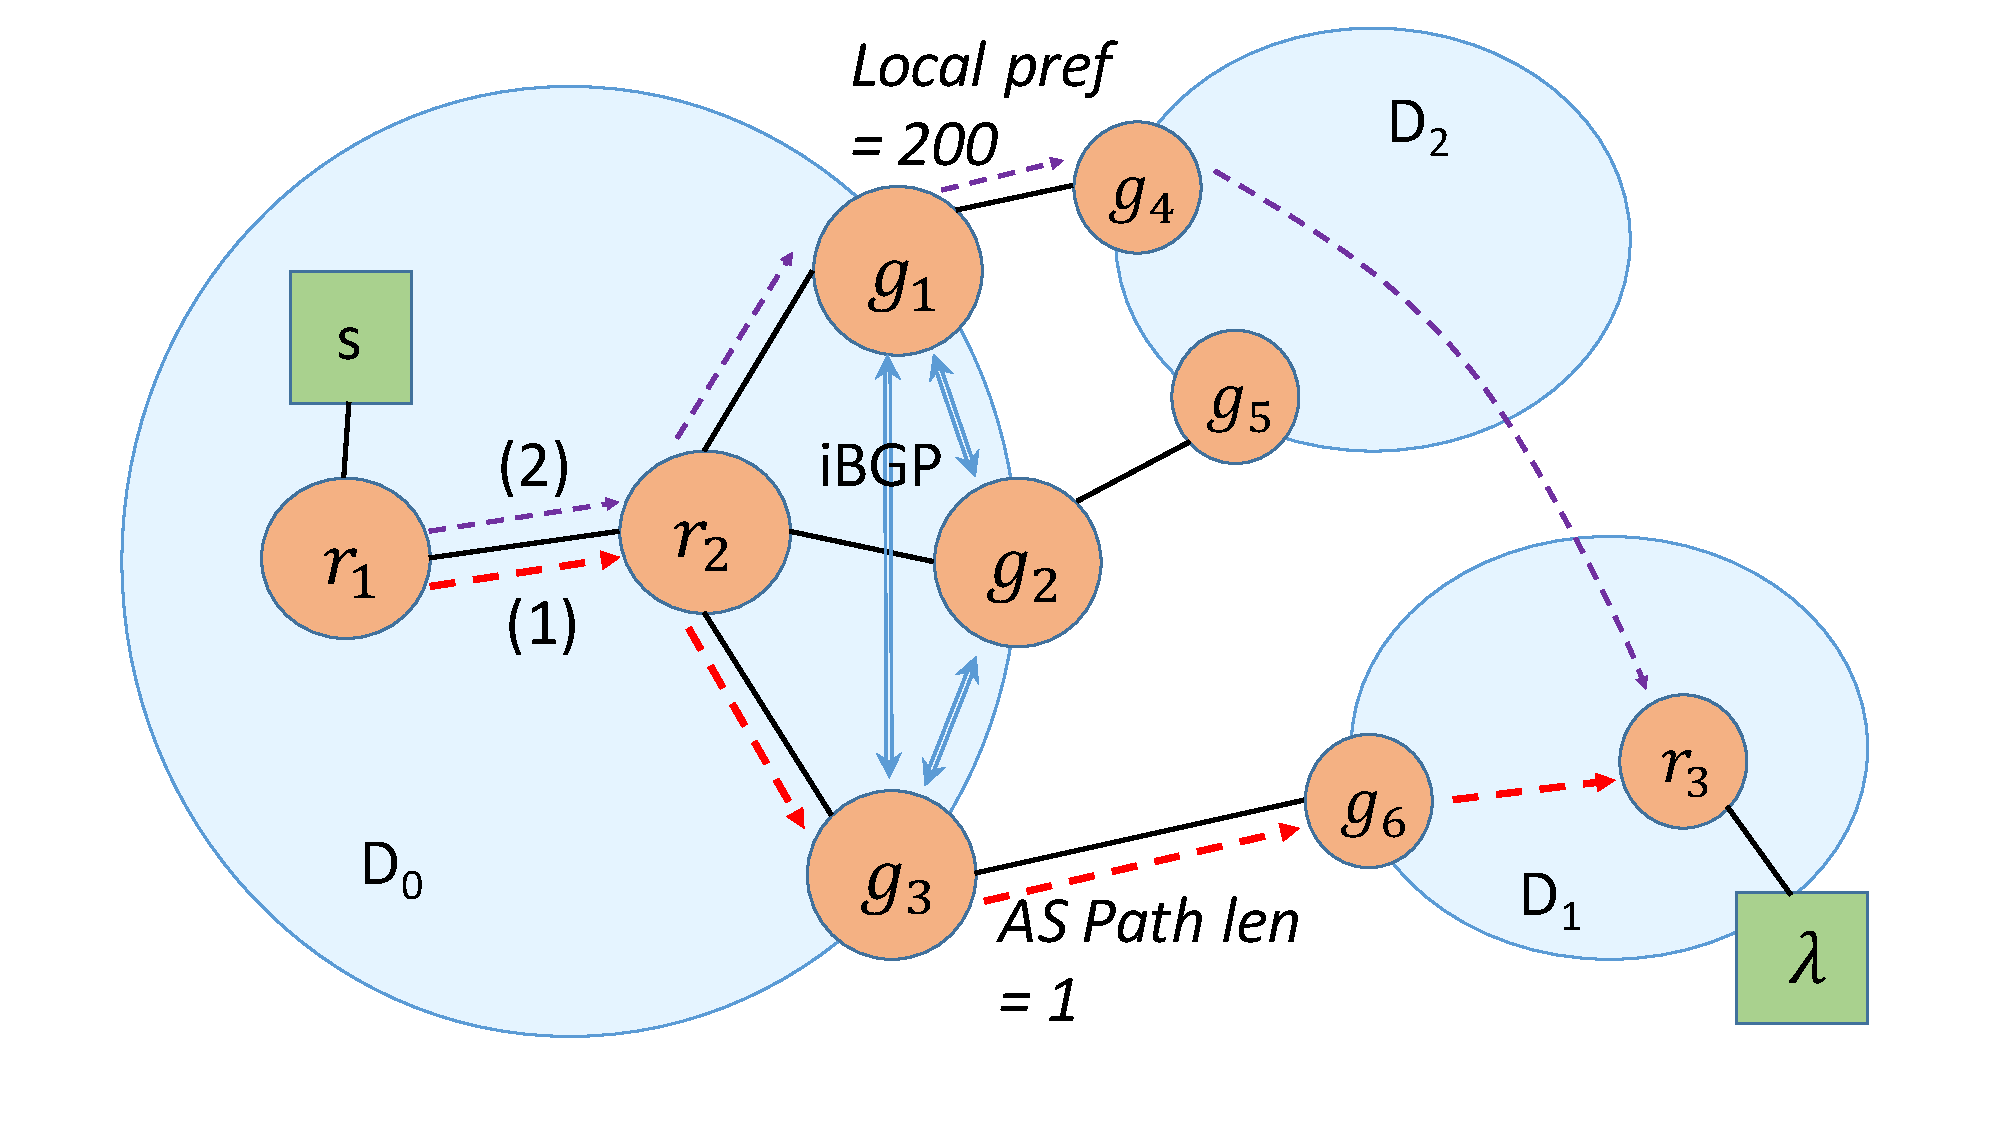
\includegraphics[width=0.305\textwidth]{figures/bgp-example.pdf}}
	\hfill
	\subfloat[Multiple BGP Gateways]{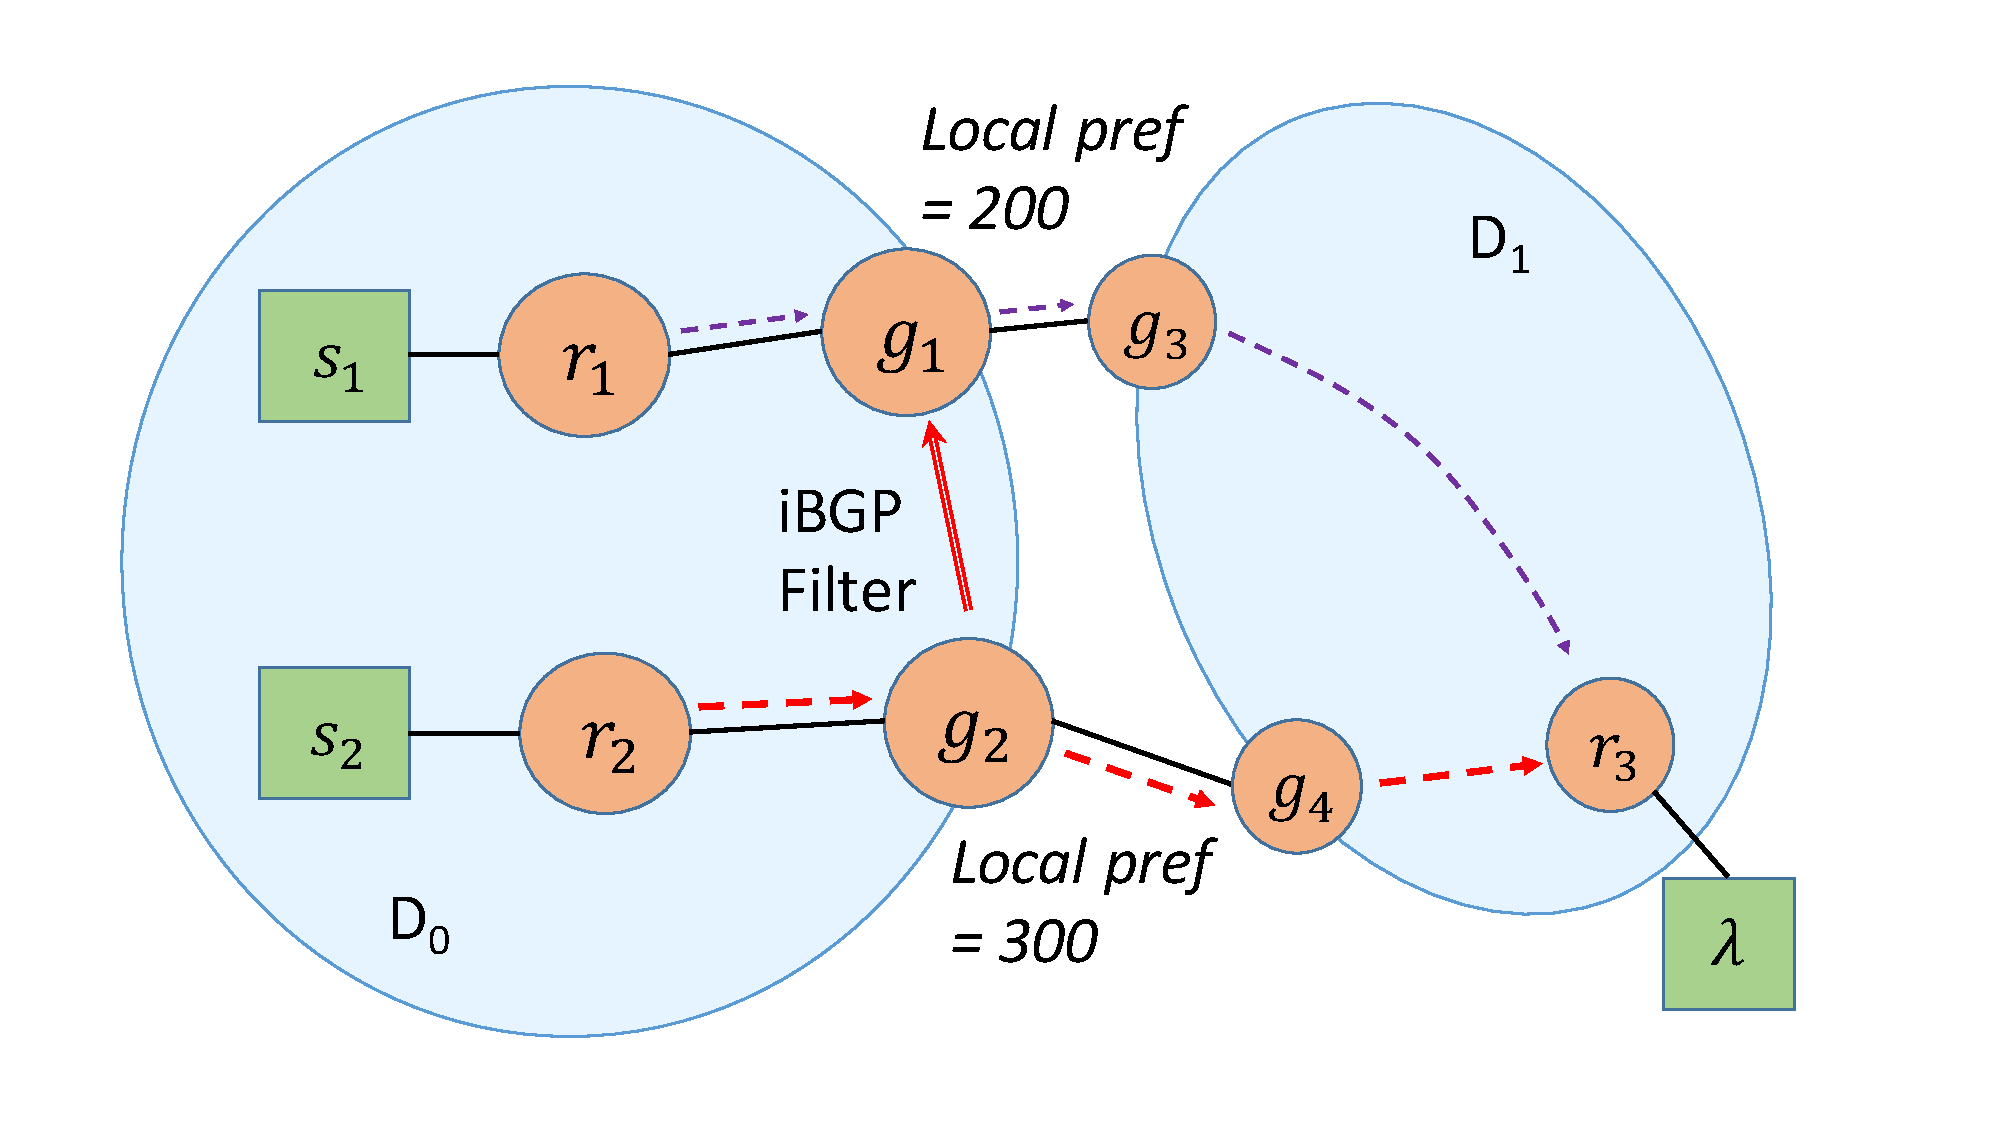
\includegraphics[width=0.31\textwidth]{figures/bgp-example2.pdf}}
	\hfill
	\subfloat[Static Routes]{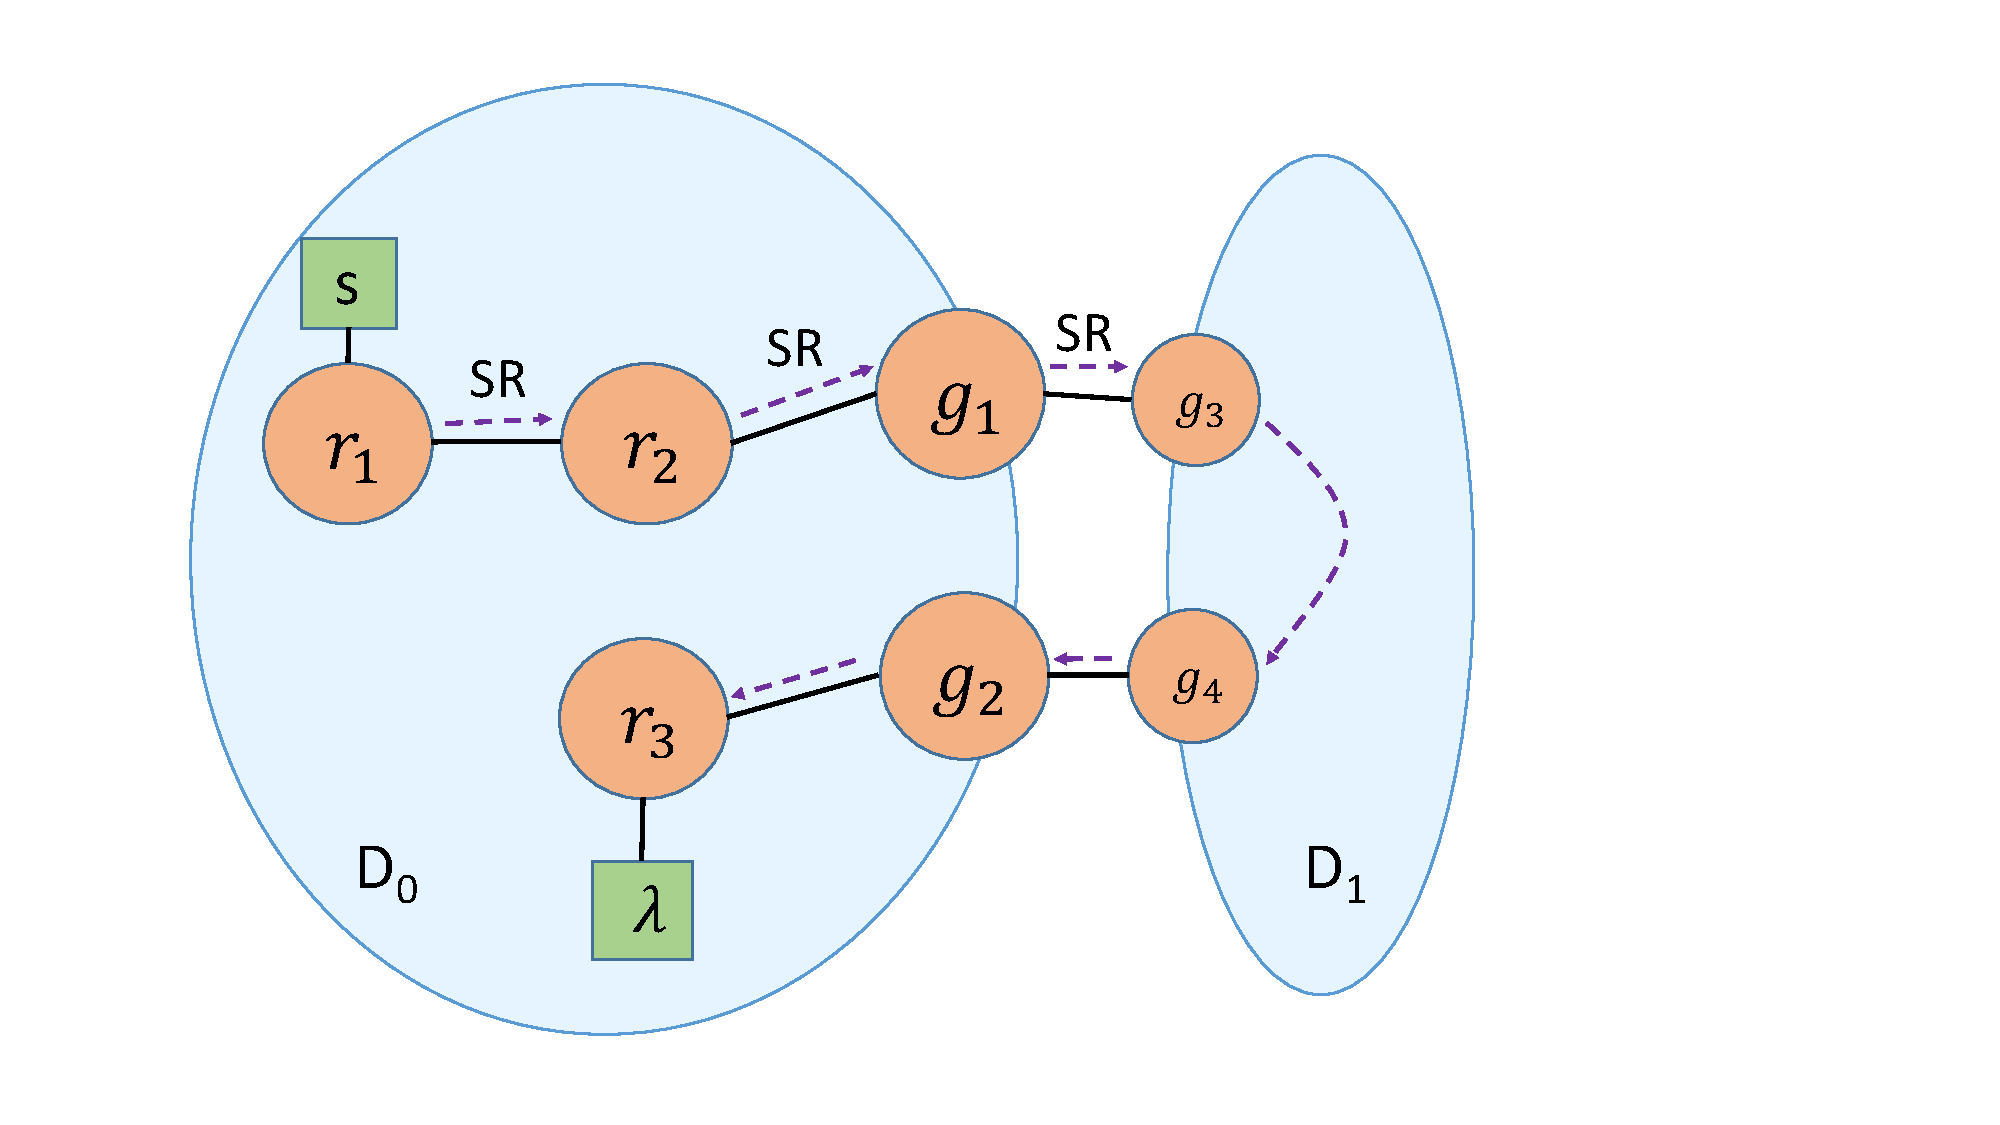
\includegraphics[width=0.265\textwidth]{figures/static-route.pdf}}
	\compactcaption{\label{fig:bgpexample}
		Examples of BGP and static route configurations for 
		inter-domain routing given domain assignment $\Theta$.}
\end{figure*}

\minisection{Configuring BGP and Static Routes}
In this section, we describe how to configure
BGP routers so that the routes chosen by BGP 
(and redistributed into OSPF) 
can yield the policy-compliant
paths $\Pi$ given as input. 
Note that, the BGP $\rightarrow$ OSPF redistribution
can sometimes lead to explosion of OSPF routing tables. However, 
in our datacenter setting, BGP is used in a restricted
sense for management ease and BGP routers are not connected
to the external internet directly, thus, only internal
prefixes are redistributed.


To enforce the policy-complaint paths, 
We need to take into account three different
cases, which are illustrated in \Cref{fig:bgpexample}.  
In the first case, path to destination $\lambda$
exits the domain through a single BGP gateway, illustrated in 
\Cref{fig:bgpexample}(a). For path (1)---i.e., the red one---
to be the chosen path, it is already on the shortest AS path, 
therefore, the gateway for $\lambda$ in domain $D_0$ is $g_3$, i.e.,
$G(0, \lambda) = g_3$. However, if path (2)---i.e., the purple one---
is the path from Genesis, it has to traverse more domains. Thus, 
we set local preference for route for $\lambda$ to $g_1$ to 200, i.e.,
$LP(g_1, g_4, \lambda) = 200$. After iBGP route distributions, the 
gateway route for $\lambda$ will be through $g_1$.
% In the first case, a path is preferred because it traverses fewer domains.
% For example, in \Cref{fig:bgpexample}(a), we want
% path (1)---i.e., the red one---to be the chosen path from source $s$ 
% to destination $\lambda$.
% Here, BGP router $g_3$ receives from $g_6$ an advertisement for a route to destination $\lambda$
% traversing only the domain $1$; this route has domain path length 1 as it only traverses 1 domain. 
% Instead, $g_1$ and $g_2$ receive advertisements for a route 
% ($D_2$, $D_1$)
% to destination $\lambda$  with 
% domain path length 2. Since our objective is to send traffic along
% $g_3$, for path (1) we do not need to add any further BGP configurations,
% and the route via $g_3$ is automatically redistributed into domain $D_0$;
% for destination $\lambda$, the gateway at domain $D_0$ is $g_3$, i.e.,
% $G(0, \lambda) = g_3$.

% In the second case, the requested path does not have shortest domain path length
% and we therefore need to set local preferences.
% For example, let's say that in \Cref{fig:bgpexample}(a) we now want
% path (2)---i.e., the purple one---to be the chosen path from source $s$
% to destination $\lambda$. 
% Since $g_1$'s route traverses more domains than
%  $g_3$'s route,
% we need to set the local preference of route received by $g_1$ 
% (from $g_4$) to a value greater than the preference for the route received by $g_3$. 
% In the example, we set the preference at node $g_1$: 
% $LP(g_1, g_4, \lambda) = 100$
% which causes $g_1$ to become gateway at domain $D_0$ for destination $\lambda$, i.e., 
% $G(0, \lambda) = g_1$.

In the second case, two paths from different sources to
destination $\lambda$ exit
the domain through two different
gateways. In \Cref{fig:bgpexample}(b),
the path from $r_1$ to $\lambda$ exits domain $D_0$ through 
gateway router $g_1$, while the path from $r_2$  to $\lambda$ exits 
through $g_2$. 
% Moreover,  we assume that $g_1$ is the closest gateway to $r_1$ and 
% $g_2$ is the closest gateway to $r_2$ w.r.t. OSPF paths in the domain.
In this case, both these routes need to be  
redistributed to the OSPF domain. 
By assigning local preferences such that
$LP(g_1,g_3,\lambda)<LP(g_2,g_4,\lambda)$,
 $g_2$ will redistribute a route for $\lambda$ 
 to the OSPF domain and
the traffic from $r_2$ will correctly exit through $g_2$. 
To prevent the traffic from $r_1$ to exit through $g_2$,
we add an iBGP filter
 for the connection $g_2 \rightarrow g_1$ for
destination IP $\lambda$. 
Thus, $g_1$ will 
redistribute the route it received from $g_3$. For 
this example, $G(0, \lambda) = \{g_1, g_2\}$. 

%\minisection{Static Routes} \label{sec:static}
Finally, we describe a case in which standard BGP cannot enforce
the desired path, therefore requiring the use of static routes.
Consider the path for destination $\lambda$ 
shown in \Cref{fig:bgpexample}(c) which has a domain loop in the path
($D_0 \rightarrow D_1 \rightarrow D_0$), thus, this path cannot be
enforced by conventional BGP routing.
% BGP Gateway $g_1$, which is in
% domain $D_0$, 
% will receive an advertisement for $\lambda$ that goes through domain
% 1 and then domain $D_0$.
% This advertisement will be rejected because it creates a loop---i.e., the domain $D_0$
% appears twice in the path. 
To circumvent this issue, \name use static routes 
(illustrated in \Cref{fig:bgpexample}(c)). 
For finding the minimal number of static routes to be used in
such cases, we find the longest path suffix which have
no domain loops (from the start of this path fragment, 
BGP+OSPF can be used for routing), 
and add static routes from the source to the start of this path suffix.
 
% In this example
% the static routes
% $SR(r_1,\lambda) = \{r_2\}$, $SR(r_2,\lambda) = \{g_1\}$, and $SR(g_1,\lambda) = \{g_2\}$ 
% guarantee that routes from $r_1$, $r_2$, and $g_2$ to $\lambda$ traverse the desired links.

% \minisection{Algorithm}
% We are now ready to describe the algorithm that,
% given a set of paths $\Pi$, determines
% BGP local preferences, iBGP filters, and static routes for enforcing such paths.
% For a path $\pi = l_1 l_2 \ldots l_m \in \Pi$, we
% can divide the path into intra-domain paths and inter-domain
% links. We express $\pi$ as 
% $\pi_1 idl_1^2 \pi_2 \ldots idl_{n-1}^n \pi_n$ where
% each subpath $\pi_i$ is completely in a
% domain, i.e., for each 
% link $(r_1,r_2) \in \pi_i \implies \Theta(r_1) = \Theta(r_2)$;
% and links $idl_1^2, idl_2^3 \ldots idl_{n-1}^n$ 
% represent the inter-domain links, i.e., 
% if $idl_i^{i+1}=(r,r')$ then $\Theta(r_1) \neq \Theta(r_2)$. 
% The domain path
% $\tilde{\pi} = d_1 \ldots d_n=\Theta(\pi_1)\ldots \Theta(\pi_n)$ describes the 
% domains traversed by $\pi$ (where
% $\Theta(\pi_i)$ denotes the domain of the routers in the 
% domain path $\pi_i$). 


% For a given path $\pi$ and corresponding path $\tilde{\pi}$,
% we find the longest non-looped domain subpath ending in domain
% $d_n$. Formally, we find the smallest index $nl$ such that
% $\forall j \geq nl. ~\neg\exists k \geq i.~d_j = d_k$. 
% The loop-free subpath $\pi'=\pi_{nl} ~idl_{nl}^{nl+1}\ldots idl_{n-1}^n \pi_n$ corresponding to
% domains $d_{nl} \ldots d_n$
% can be induced using BGP, as described in \Cref{fig:bgpexample}(a)
% and \Cref{fig:bgpexample}(b).
% For all links that are not in $\pi'$
% we will require static routes.
% With abuse of notation, for every link $(r_1,r_2)\in\bigcup_{i< nl} \pi_i\cup \bigcup_{i< nl}\{l_i^{i+1}\}$ 
% we have
% $SR(r_1, \lambda) = \{r_2\}$. 
% For a domain assignment $\Theta$, the 
% inter-domain static routes we place
%  are necessary, can be  computed easily, and cannot be further minimized.
% However, 
% finding optimal static routes for the intra-domain configurations remains a
% hard problem. 

% Finally, for each intra-domain subpath
%  that is not statically routed, \name applies
% OSPF synthesis with certain modifications.
% This is done after aggregating 
% by domain across all subpaths obtained 
% when processing all paths in $\Pi$.
% We describe this in the next section.
%For each destination $\lambda \in \Lambda$, 
%BGP is configured accordingly
%based on if there is a single gateway in domain (\Cref{fig:bgpexample}(a))
%or multiple gateways (\Cref{fig:bgpexample}(b)) for the paths of destination
%$\lambda$ in the domain. 


%Static routes have the highest priority and is used to 
%exit and enter a domain multiple times. 
%While static routes
%do not reduce the resilience of the network (all routes are still
%enabled, unlike route filters), a network under flux will have
%unpredictable routing behaviour, unlike with only OSPF and BGP
%configured at the routers. 
%Also, static routes have to be installed per-destination, thus increasing
%the size of configurations drastically as number of policy paths increase.
%
%Given a path $p$ for subnet $\lambda$ and 
%the corresponding domain path $p_{as}
%= as_1 \rightarrow as_2 \rightarrow \ldots \rightarrow as_m$ (where
%$as_m = \Theta(\lambda)$), static
%routes are required if $p_{as}$ has a domain-loop. 
%To minimize
%the number of static routes, we find 
%the smallest $i \in [1,m]$ 
%such that $\overline{p_{as}} = as_i \rightarrow as_{i+1}
%\rightarrow \ldots \rightarrow as_m$ has no loops. 
%Therefore, $\overline{p_{as}}$ is the longest domain-loop-free
%subpath of $p_{as}$, and be can be enforced using BGP and OSPF. For the 
%network path corresponding to domain path $as_1 \rightarrow as_2 
%\rightarrow \ldots \rightarrow as_{i-1}$, we require static
%routing rules for each next-hop. The static routing score
%is the total number of static route hops required to enforce
%the input paths.
%\todo{Write about the BGP paths are extracted for the next phase}
%
%\subsubsection{BGP Local Preference Entries}
%\name uses BGP local preference to route traffic
%for a particular subnet to the next domain via a specific 
%gateway as per the input paths obtained. 
%As shown in \Cref{} (Refer
%to ex), if there are multiple exit gateways from an domain 
%for a subnet $\lambda$, we require local preference entries at the 
%gateways and iBGP filters among these gateways for $\lambda$.
%
%For a domain $d$ and subnet $\lambda$, consider the set 
%of paths to $\lambda$ exiting $d$ using BGP (and not statically
%routed as described in \Cref{sec:static}). Let $E$ denote the
%set of exit gateway routers for the paths of $\lambda$. 
%If $|E| = 1$, if gateway $g$ receives a route with 
%strictly shortest domain path length (\Cref{alg:bgppathrules}) 
%which enforces the paths
%for $\lambda$, we do not need to configure local preference
%entries on any BGP router in the domain for $\lambda$. If
%the exit route chosen by the gateways for $\lambda$ does not 
%enforce the paths, \name configures a local preference entry
%for $\lambda$ at exit gateway, and thus, the exit route chosen
%by BGP enforces the input paths for $\lambda$ in the domain.
%
%If $|E| ~> 1$, multiple BGP routes must be redistributed to 
%the OSPF domain.
%E local prefs + E(E - 1) iBGP filters!
%

\minisection{Modified OSPF Synthesis}
When BGP routes for destination $\lambda$ 
are redistributed by multiple gateways to an 
OSPF domain, \name uses a modified OSPF synthesis
algorithm from \secref{sec:intra-synthesis}.
% to assign OSPF weights to the links in each domain
% and place static routes. 
In case of multiple gateways, an OSPF router will choose
the closest BGP gateway in terms of OSPF distance 
for $\lambda$. For instance, a router $r$ will choose
gateway $g_1$ over $g_2$ if the OSPF distance from $r$ to $g_1$ 
is strictly lesser than the distance from $r$ to $g_2$. 
We add new constraints on OSPF weights (details omitted for brevity) 
to ensure that any router on the path is closest to the gateway in the path.
% Assume we are given the input subpath $\pi_i=r \rightarrow^+ g_1$ in
% the domain $\theta$ for some destination $\lambda$ outside
% of $\theta$; this path should exit through gateway $g_1$. 

% Assume a subpath in domain $\theta$ for destination $\lambda$
% as follows: $r \rightarrow r_1 \rightarrow \ldots \rightarrow g$. 
% For the set of gateway
% routers $G(\theta, \lambda)$ 
% for destination $\lambda$ and domain $\theta$,
% \name adds the following constraints to ensure
% router gateway $g$ is closest to router $r$ than
% any other router $g' \in G(\theta, \lambda)$ :
% we define the relation $r_1 \rightarrow^+_{\xi_{\lambda}} r_2$, which holds if
% $r_2$ is reachable from $r_1$ in the destination tree $\xi_\lambda$.
% For each subpath $r \rightarrow^+_{\xi_{\lambda}} g$ to destination $\lambda$
% and for each $g' \in G(\theta, \lambda)$ such that $g\neq g'$,
% \begin{equation} \label{eq:gateway}
% \forall r' \in N(r) \setminus \{r_1\}.~
% \sum_{\mathclap{r \rightarrow r_1 \ldots g }}~W < 
% W(r, r') + D(r', g')
% \end{equation}
% If one of the constraints of Equation~\ref{eq:gateway}
% is part of an unsat-core, 
% adding the static route $(r, r_1)$ 
% to $SR(\lambda)$ eliminates the unsatisfiability caused by  
% the constraint. Effectively, while $g'$ is closer to
% $r$ than $g$, we use the static route to steer traffic toward $g$. 

% \minisection{Soundness and Completeness}
% For a network topology $T$ and 
% fixed domain assignment $\Theta$, \name's path-compliance
% synthesis is \emph{sound}---i.e., for input $(PC, \Pi)$, the 
% synthesized configuration 
%  induces all paths in $\Pi$. 
% \name's soundness is by virtue of the BGP forwarding semantics specified in ~\Cref{alg:bgppathrules}
% and \Cref{thm:ospfsr}---OSPF and static routes in a domain 
% forward traffic to the specified gateway, where BGP is configured to 
% send it to the next domain in the path. 
% The same completeness considerations as for Section~\ref{sec:ospfsr} also hold here
% and completeness can be obtained by running \Cref{alg:unsat} in each domain multiple times and choosing different
% unsatisfiable cores and static routes assignments.
%!TEX root = paper.tex
\section{From Waypoint Policies to Policy-Resilient Configurations}
\label{sec:waypointres}


The algorithm we presented in the previous section can generate configurations
for complex types of policies and at the same time can achieve good
connectivity resilience.
In this section, we present a different algorithm that, for a restricted set of policies,
can synthesize configurations with high \emph{policy-resilience}.
In particular, we focus on \emph{waypoint policies}
which play a crucial role in enterprise and
datacenter networks for security, performance,  
and auditing.

\subsection{Problem Setup}

We consider policies of the form 
\texttt{$\lambda$: s >> $\waypt$ >> t}
where $\lambda$ is a destination IP subnet,  
$s$ and $t$ are the source and destination routers respectively, 
and $\waypt \subseteq V$ is a set of routers called the \emph{waypoint set}. 
Each policy is mapped to a packet class and
we say that a configuration complies to a policy for $pc$ if 
at least one of the induced paths in $\paths^C(pc)$ 
traverses one waypoint $w \in \waypt$.
\footnote{
The attentive reader will note that in our definition of waypoint-compliance 
we do not require all induced paths for $pc$ to traverse the waypoints. 
Our definition can be realized by two mechanisms: 1) A router
which has multiple routes for $\lambda$ will split the traffic
among these routes, and 2) The waypoint can mark certain fields in
the packet header, and the network operator can employ 
simple edge-based checks at the destination 
(for e.g., in the hypervisor) to 
detect if a packet traversed the waypoint or not. Thus, only
packets which traversed a waypoint-compliant path would be 
accepted and forwarded to the tenant. 
}
Here, $\waypt$
can be the set of physical replicas of,  for example, a firewall.


 Given a set of such waypoint policies, our goal is to
find a policy-compliant configuration 
$C=(T,\Theta,W,LP$, $IF,SR)$ 
with high policy-resilience. Ideally, for 
any single link failure, there should be at least 
one path to $\lambda$ which is waypoint-compliant. 
In the following section, we focus on 
intra-domain configurations,
and present an algorithm
that solves this problem when the network 
has a single domain.
When the network has multiple domains, 
we assume that all waypoints
belong to the same domain and
use our new algorithm in the domain 
which contains the waypoints.  
Our assumption that all waypoints lie in the 
same domain can be realized
through Network Function Virtualization~\cite{opennf, netbricks},
which provides waypoint replication and 
 flexible waypoint placement in the network.


%\todo{explain why we don't do inter, seems like first para from next section
%should be somewhere here}

%
%\loris{somewhere describe how it's a two-phase approach
%and now all the paper is about 1-resilience so don't say
%1 resilience everywhere}

%\todo{not sure where following text belongs}
%Support for  
%middlebox traversals is commonly 
%provided by network operators.
%Network Function Virtualization (NFV) has been a 
%major driving force for providing reliability 
%guarantees under failures  
%for middlebox traversals~\cite{opennf, netbricks}. 
%Using NFV technology, operators can replicate 
%their middleboxes across the network for providing 
%resilience guarantees. 





%\subsection{Problem Statement}
%Let us consider an 
%unordered waypoint policy of the form: 
%\texttt{$\lambda$: s >> $\waypt$ >> t},
%where $\lambda$ is the destination IP subnet,  
%$s$ and $t$ are the source and destination router respectively, 
%and $\waypt \subseteq V$ is the waypoint set. This
%policy is mapped to a packet class $pc \in \nat$. 



\subsection{Intra-domain Policy-Resilient Waypoint Compliance}\label{sec:ospfwaypoint}
We use \genesis's
support for isolation to generate two switch-disjoint paths
which are waypoint-compliant with respect to $\waypt$. A single link
failure will not disable both these paths
and we could guarantee policy-resilience by 
guaranteeing that, under any link failure,
traffic to $\lambda$ 
traverses one of these two paths. However, enforcing the control plane to 
always route through one of the two paths is difficult and overly 
restrictive. 
Instead, we relax our constraints to guarantee that
the two paths are shorter than any non-compliant path in 
the network. The existence of two such paths still guarantees that 
traffic
under any single link failure,
 traverses a waypoint. 



\subsubsection{Waypoint-Compliance Constraints} \hspace*{4mm}


\label{sec:waypoint-compliance-constraints}
We now show how to generate constraints that
guarantee that a single waypoint-compliant path is shorter
than any path which does \emph{not} traverse a waypoint. 
We define $D(s,t,\waypt)$ to be the 
distance between $s$ and $t$ for path that \emph{do not}
 traverse any waypoint $w \in \waypt$.
We call  $D(s,t,\waypt)$ the \emph{non-waypoint distance}.
  We add constraints to represent these distances by
  considering a network topology where all the  
  waypoints $w \in \waypt$ are removed:
\begin{equation} \label{eq:wdistance}
\forall s, t \in V \setminus \waypt. ~\forall r \in N(s) \setminus \waypt.~
D(s, t, \waypt) \leq W(s, r) + D(r,t,\waypt)
\end{equation}
%These constraints are similar to the constraints specified in
%\Cref{eq:distance}, but for an ``altered'' topology where all
%the waypoint routers are removed, and thus, any path in this 
%topology is not compliant with the waypoint policy. 
Using these equations,
$D(s,t,\waypt)$ is upper bounded by the actual shortest non-waypoint distance from $s$ to $t$.

\definecolor{orange}{RGB}{255, 157, 30} 

Given a destination tree $\xi_\lambda$, we can use
non-waypoint distances to enforce waypoint-compliance. Consider a 
router in $r$ such the waypoint $w \in \waypt$ is downstream to $r$ in $\xi_\lambda$---i.e.,
there exists a path from $r$ to $w$ in $\xi_\lambda$.
The path from $r$ must traverse through 
a waypoint in $\waypt$.  
If the sum of weights of the edges of
the path in the tree $r \rightarrow^+_{\xi_\lambda} R_\lambda$  
is strictly smaller than the non-waypoint 
distance from $r$ to $R_\lambda$, 
then the path from $r$ to $R_\lambda$ is guaranteed to traverse
a waypoint $w \in \waypt$. These constraints are expressed as:
\begin{equation} \label{eq:waypoint}
\forall r' \in N(s) \setminus N_{\xi_\lambda}(r).~~ \sum_{\mathclap{\substack{r \rightarrow^+_{\xi_\lambda} R_\lambda}}} 
W < 
W(r, r')+ D(r', R_\lambda, \waypt) 
\end{equation}

\begin{figure}[!t] 
	\centering
	\subfloat[Waypoint-compliant edge weights]{
		\resizebox {0.45\columnwidth} {!} {
			\begin{tikzpicture}[shorten >=0.5pt,node distance=,on grid,auto,
			square/.style={regular polygon,regular polygon sides=4}] 
			\node[state] at (0,0) (s)  {$s$}; 
			\node[state, fill=orange] at (1.5,1) (v1)  {$r_1$}; 
			\node[state, fill=orange] at (1.5,-1) (v2)  {$r_2$}; 
			\node[state] at (3, 0)(t) {$t$};
			\node[state, rectangle] at (4, 0) (d1) {$\lambda$};
			\path[->] 
			(s) edge [red] node [black] {1} (v1)
			(s) edge  node {1} (v2)
			edge  node [above] {10} (t)
			(v1) edge [red] node [black] {5} (t)
			(v2) edge  node [black] {1} (t)
			(t) edge [red, dashed] node {} (d1);
			\end{tikzpicture}
		}}
		\hspace*{4mm}
		\subfloat[Routing Loop]{
			\raisebox{0.7cm}{\resizebox {0.45\columnwidth} {!} {
					\begin{tikzpicture}[shorten >=0.5pt,node distance=,on grid,auto,
					square/.style={regular polygon,regular polygon sides=4}] 
					\node[state] at (0,0) (s)  {$s$}; 
					\node[state] at (1.5,1) (v1)  {$r_1$}; 
					\node[state] at (3, 0)(t) {$t$};
					\node[state, rectangle] at (4, 0) (d1) {$\lambda$};
					\path[->] 
					(s) edge [red] node [black, sloped, anchor=center, above]
					{$sr(\lambda)$} node
					[black, sloped, anchor=center, below] {1} (v1)
					edge  node [below] {5} (t)
					(v1) edge [red] node [black] {50} (t)
					(t) edge [red, dashed] node {} (d1);
					\end{tikzpicture}
				}}}
				\compactcaption{Example of waypoint-compliant edge weights 
					and example of a routing loop caused by a static route.} \label{fig:ospfloop}
\end{figure}



These equations do \emph{not} guarantee that
router $r$ will forward traffic to  
$N_{\xi_\lambda}(r)$.
Consider the example in \Cref{fig:ospfloop}(a) where traffic for
$\lambda$ must traverse through one of the waypoints in $\{r_1, r_2\}$. 
In this case,  \genesis provided the path $s \rightarrow 
r_1 \rightarrow t$, but  
the shortest path is $s \rightarrow r_2
\rightarrow t$ which is waypoint-compliant.


\iffull
\begin{theorem}[OSPF Waypoint Soundness] \label{thm:waypoint}
	Given a set of waypoint paths $\{(\pi_{pc}, \waypt_{pc}) ~|~ pc\}$, if edge weights 
	$W$ satisfy constraints (\ref{eq:wdistance}) and (\ref{eq:waypoint}), for
	each packet class $pc$, the shortest path between its endpoints
	traverses one of the waypoints in $\waypt_{pc}$.
\end{theorem}
\begin{theorem}[OSPF Waypoint Soundness] \label{thm:waypoint}
	Given a set of waypoint paths $\{(\pi_{pc}, \waypt_{pc}) ~|~ pc\}$, if edge weights 
	$W$ satisfy constraints (\ref{eq:wdistance}) and (\ref{eq:waypoint}), for
	each packet class $pc$, the shortest path between its endpoints
	traverses one of the waypoints in $\waypt_{pc}$.
\end{theorem}
\iffull
\begin{proof}
	Let us assume there exists a packet class $pc$ with waypoint set $\waypt_{pc}$ 
	and waypoint path $\pi_{pc} = (s_{pc}, s_1)(s_1, s_2)\ldots (s_n, d_{pc})$, 
	such that  the 
	shortest path $\sigma_{pc}=(s_{pc}, r_1)$ $(r_1, r_2)\ldots (r_m, d_{pc})$ 
	is not waypoint-compliant---i.e.,  
	for every $i$, we have $r_i\not\in \waypt$.	
	Since $\sigma_{pc}$ is the shortest weighted path: 
	\begin{equation} \label{eq:wassumption}
	\sum_{\pi_{pc}} W \geq \sum_{\sigma_{pc}} W
	\end{equation}

	
	Let $s_i \not= r_i$ be the first point of divergence of the paths---i.e., for every $j<i$, $s_{j} = r_{j}$.
Constraints (\ref{eq:waypoint}) impose 
$(s_{i-1}, s_i)\ldots(s_n, d)$ to be 
shorter than any path which is not waypoint-compliant. 
Let us consider the neighbour router $r_1$ in $\sigma_{pc}$:
	\[
	\sum_{\mathclap{\substack{(s_{i-1}, s_i)\cdots(s_n, d)}}} 
	W < W(s_{i-1}, r_i)+ D(r_i, d, \waypt_{pc})
	\]
	Since $\sigma_{pc}$ does not traverse any waypoint in $\waypt_{pc}$,
	we use constraints (\ref{eq:wdistance}) 
	to expand the terms $D(r_k, d_{pc}, \waypt_{pc})$ for $i \leq k \leq m$:
	\[
	\sum_{\mathclap{\substack{(s_{i-1}, s_i)\cdots(s_n, d)}}} 
	W < W(s_{i-1}, r_i)+ W(r_i, r_{i+1}) + D(r_{i+1}, d,\waypt_{pc})
	\] 
	\begin{center}
		$\ldots$
	\end{center}
	\[
	\sum_{\mathclap{\substack{(s_{i-1}, s_i)\cdots(s_n, d)}}} 
	W < W(s_{i-1}, r_i)+ W(r_i, r_{i+1}) + \ldots W(r_{m}, d) + D(d, d, \waypt_{pc})
	\] 
	\[
	\sum_{\mathclap{\substack{(s_{i-1}, s_i)\cdots(s_n, d)}}} 
	W \hspace{0.4cm}< \hspace{0.4cm}
	\sum_{\mathclap{\substack{(r_{i-1}, r_i)\cdots(r_m, d)}}} 
	W
	\]
	Adding $\Sigma_{(s, s_1)\cdots(s_{i-2},s_{i-1})}$ to both sides:
	\[
	\sum_{\mathclap{\substack{\pi_{pc}}}} 
	W < 
	\sum_{\mathclap{\substack{\sigma_{pc}}}} 
	W
	\] 
However, this contradicts the assumption (\ref{eq:wassumption}) that 
$\sigma_{pc}$ is the shortest path from $s_{pc}$ to $d_{pc}$. 
%Hence, proved, there is no path $\sigma_{pc} \in \paths^C(pc)$ such that $\forall w \in \waypt.~
%w \not\in \sigma_{pc}$. 
\end{proof}
\fi
\paragraph{Completeness}
In this setting, the notion of completeness is slightly complicated as
we solve a different variant of the path synthesis problem.
If the problem admit solution, there always exists a set of waypoint-compliant
paths on which the proposed technique returns appropriate weights.
However, if we might provide the algorithm with waypoint-compliant paths
for which no $W$ satisfy constraints (\ref{eq:waypoint}), although a waypoint-compliant
configuration exists. 
Formally, even if $\pi_{pc}$ is greater than the non-waypoint distance between the endpoints of $pc$, thus,
violating constraints (\ref{eq:waypoint}), the shortest path could still traverse one of the waypoints in $\waypt_{pc}$.
\fi

\minisection{Soundness and Completeness}
If edge weights satisfy constraints (\ref{eq:wdistance}) and (\ref{eq:waypoint}), 
then paths for packet classes will traverse one of the waypoints. However, these
constraints do not ensure completeness---i.e., a solution could be waypoint-compliant
while violating some of the constraints, specifically constraint (\ref{eq:waypoint}):
while the weight of the Genesis path may be greater than the non-waypoint distance, 
the actual shortest path could be waypoint-compliant.

% In this setting, the notion of completeness is slightly complicated as
% we solve a different variant of the path synthesis problem.
% If the problem admit solution, there always exists a set of waypoint-compliant
% paths on which the proposed technique returns appropriate weights.
% However, if we might provide the algorithm with waypoint-compliant paths
% for which no $W$ satisfy constraints (\ref{eq:waypoint}), although a waypoint-compliant
% configuration exists. 
% Formally, even if $\pi_{pc}$ is greater than the non-waypoint distance between the endpoints of $pc$, thus,
% violating constraints (\ref{eq:waypoint}), the shortest path could still traverse one of the waypoints in $\waypt_{pc}$.

\subsubsection{Avoiding Routing Loops} \label{sec:loopavoidance} \hspace*{4mm}


\Cref{alg:wayptunsat} presents the OSPF 
synthesis algorithm with static routes.  
If one of the constraints in \Cref{eq:waypoint} is part of an unsatisfiable  
core, \name adds the static 
route
 $(r, N_{\xi_\lambda}(r))$ to
$SR(\lambda)$ to eliminate the equations at router $r$. 
Constraints (\ref{eq:waypoint}) does not 
guarantee that the path generated
by \genesis is indeed the shortest path, so adding
static routes can lead to undesired behaviors like routing loops.  
Consider the example configuration shown in \Cref{fig:ospfloop}(b).
If link $r_1 \rightarrow t$ fails, traffic will oscillate between 
$s$ and $r_1$ due to SR and OSPF and finally be dropped. 
% Traffic for $\lambda$ at router $s$ is forwarded to $r_1$ because of the
% static route at $s$. At router $r_1$, the shortest OSPF route to
% $\lambda$ is $r_1 \rightarrow s \rightarrow t$ with weight 6 (compared 
% to $r_1 \rightarrow t$ of weight 50). Thus, $r_1$ will send the 
% packet back to $s$  causing a routing loop as $s$ will send
% it back to $r_1$ and back and forth till the \emph{ttl} (time to live) of the
% packet expires. 

Whenever \name adds a static route to resolve an unsat-core,
it removes the constraints pertaining to 
the static route and \emph{adds} new constraints to prevent
routing loops. 
%This
% approach ensures we do not add superfluous constraints for links
%that do not contain a static route in the final configuration 
%and cannot cause routing loops. 
Suppose \name added a static route $(sr_1, sr_2)$ for destination
$\lambda$ where $sr_2 = N_{\xi_\lambda}(sr_1)$ (because we do not add
static routes on any other links except $\xi_\lambda$). \name needs to
ensure that, for any router $r\in\xi_\lambda$ that does not 
lie in the downstream path $sr_2 \rightarrow^+_{\xi_\lambda} R_\lambda$, 
the shortest path from $sr_2$ to $R_\lambda$ does not traverse through 
$r$. For example, 
in \Cref{fig:ospfloop}(b), there is a routing loop because
 the shortest path from $r_1$ to $t$ 
 goes through upstream router $s$.

Formally, \name adds constraints to 
ensure that the weight
of path $sr_2 \rightarrow^+ R_\lambda$ is 
strictly smaller than any path from $sr_2$ that traverses a
router $r'$ not in the downstream path from $sr_2$: 
\begin{equation} \label{eq:rla}
\forall r' \in \xi_\lambda. ~sr_2 \not\rightarrow_{\xi_\lambda}^+ r'. 
\hspace{0.3cm}\sum_{\mathclap{\substack{sr_2 \rightarrow^+ R_\lambda}}} 
W < D(sr_2, r') + D(r', R_\lambda) 
\end{equation}

If one of these constraints is part of an unsatisfiable
core, then there is a routing 
loop caused from $sr_2$. 
\name rectifies this 
by adding a static route 
$(sr_2, N_{\xi_\lambda}(sr_2))$ to $SR(\lambda)$. 
\Cref{alg:wayptunsat} describes the unsat-core learning algorithm
for waypoint-compliance.

\iffull
\begin{theorem}[OSPF+SR Waypoint Soundness] \label{thm:wayptsr}
	Given a set of waypoint paths \linebreak
	$\{(\pi_{pc}, \waypt_{pc}) ~|~ pc\}$,
	\Cref{alg:wayptunsat} outputs a configuration $C(W,SR)$ 
	such that, for every packet class $pc$, 
	there exists a path in $\paths^C(pc)$ that
	traverses one of the waypoints in $\waypt_{pc}$.
\end{theorem}
%!TEX root=paper.tex
\begin{theorem}[Soundness]
	Given a set of waypoint paths $\{(\pi_{pc}, \waypt_{pc}) ~|~ pc\}$,
	\Cref{alg:wayptunsat} outputs a configuration $C(W,SR)$ 
	such that, for every packet class $pc$, 
	there exists a path in $\paths^C(pc)$ that
	traverses one of the waypoints in $\waypt_{pc}$.
\end{theorem}
\kausik{This proof is quite long, and is complicated
by the fact that we dont enforce a particular path, 
and static routes, which force me to enumerate a lot of 
cases, I will think if there is an easier proof than the 
half-completed one I have below. But I am pretty sure that 
the theorem is correct.}
\begin{proof}
	Let us assume there exists a packet class $pc$ 
	with destination $\lambda$, 
	waypoint set $\waypt_{pc}$,
	and waypoint path $\pi_{pc} = (s_{pc}, s_1)(s_1, s_2)\ldots (s_n, d_{pc})$, 
	such that for $pc$, 
	there exists no path in $\paths^C(pc)$
	which is waypoint-compliant. There are two
	cases: either there exists no path in $\paths^C(pc)$ 
	or the paths do not traverse any waypoint in $\waypt_{pc}$.

	\paragraph{Case 1:} $\paths^C(pc) = \emptyset$---i.e., there
	is a routing loop caused by static routes (OSPF forwarding
	is loop-free).
	We denote the set of static routes for $\lambda$ by $SR(\lambda)$. Note that
	multiple packet classes can share the same destination IP
	and destination router, and we 
	construct a destination-based tree from these paths, denoted by 
	$\xi_\lambda$ 

	Let us denote the routing loop as 
	$(r_0, r_1) (r_1, r_2) \ldots (r_{n-1}, r_0)$.
	Since, the path is a loop with atleast one static route,
	there must exist one router $r_i$ in the loop
	such that $(r_{i-1}, r_i) \in SR(\lambda)$ and the
	next router in the loop $r_j$ which has a static route
	$(r_j, r_{j+1}) \in SR(\lambda)$ and $r_j$ is not downstream
	to $r_i$ in $\xi_\lambda$ (meaning there is no directed path 
	from $r_i$ to $r_j$ in $\xi_\lambda$). 

	Consider $r_i$. The path from $r_i$ to $r_j$ is 
	due to OSPF forwarding, therefore, there exists a 
	path $\sigma =
	(r_i, r_{i+1})\ldots(r_{j-1}, r_j)(r_j, l_1) \ldots (l_{o}, d_{pc})$
	which is the shortest path  from $r_i$ to $d_{pc}$. 

	Since static routes are only added on edges in $\xi_\lambda$, 
	let us denote the path from $r_{i}$ to $d_{pc}$ in 
	$\xi_\lambda$ as $(r_{i}, u_1)(u_1, u_2)\ldots(u_p, d_{pc})$. 
	Consider constraint (\ref{eq:rla}) which is added for static route 
	$(r_{i-1}, r_i)$ and non-downstream router $r_j$:
	\[
	\sum_{\mathclap{\substack{(r_{i}, u_1)\ldots(u_p, d_{pc})}}} 
	W < D(r_i, r_j) + D(r_j, d_{pc}) 
	\]
	Using distance constraints (\ref{eq:distance}), we can expand 
	$D(r_i, r_j)$ and $D(r_j, d_{pc})$ along the paths 
	$(r_i, r_{i+1})\ldots(r_{j-1}, r_j)$ and $(r_j, l_1) \ldots (l_{o}, d_{pc})$
	respectively. 
	\[
	\sum_{\mathclap{\substack{(r_{i}, u_1)\ldots(u_p, d_{pc})}}} 
	W < \hspace{0.8cm} \sum_{\mathclap{\substack{(r_i, r_{i+1})\ldots(r_{j-1}, r_j)}}}W \hspace{0.6cm} + 
	\hspace{0.6cm} \sum_{\mathclap{\substack{(r_j, l_1) \ldots (l_{o}, d_{pc})}}}W  
	\]
	However, this contradicts the assumption that $\sigma$ is 
	the shortest path from $r_i$ to $d_{pc}$. 

	\paragraph{Case 2:} All paths in $\paths^C(pc)
	\not=\emptyset$ are not waypoint-compliant. 
	Let $\sigma_{pc} = (s_{pc}, r_1)(r_1, r_2) \ldots
	(r_n, d_{pc})$ be one such path in $\paths^C(pc)$.
	Given the routing function $\route^C$ constructed from $SR$ and
	$W$ (\secref{sec:routingmodel}), let the first router where routing diverges from $\pi_{pc}$ be $s_p$---i.e.,  
	$s_{p+1} \not\in \route^C(s_{p}, \lambda_{pc})$. 
	\Cref{alg:wayptunsat} on line \ref{line:waypoint} adds the following
	constraint to ensure the sub-path of $\pi_{pc}$ 
	from $s_{p}$ to $d_{pc}$ is shorter than non-waypoint paths:
	\begin{equation} \label{eq:wuniq}
	\sum_{\mathclap{\substack{(s_{p}, s_{p+1})\cdots(s_n, d_{pc})}}} 
	W < W(s_{p}, r_{p+1})+ D(r_{p+1}, d_{pc}, \waypt_{pc})
	\end{equation}

	\Cref{alg:wayptunsat}
	only removes a subset of the waypoint and loop constraints
	constraints and 
	not the distance constraints (\ref{line:wremoveconstraint}). We further consider 
	two sub-cases: whether \Cref{alg:wayptunsat}
	removes Constraint (\ref{eq:wuniq}) or not. 

\begin{description}
	\item[Case 2A:]
	\Cref{alg:wayptunsat} does not remove Constraint (\ref{eq:wuniq}). 
	Thus, there is no static route $(s_p, s_{p+1})$ for
	$\lambda_{pc}$ (line \ref{line:wstaticroute}), and 
	OSPF-based forwarding occurs at $s_{p}$. 
	Since $\sigma_{pc}$ does not traverse any 
	waypoint in $\waypt_{pc}$,
	we use constraints (\ref{eq:wdistance}) 
	to expand the terms $D(r_k, d_{pc}, \waypt_{pc})$ for $p+1 \leq k \leq m$:
	\[
	\sum_{\mathclap{\substack{(s_{p}, s_{p+1})\cdots(s_n, d_{pc})}}} 
	W < W(s_{p}, r_{p+1})+ W(r_{p+1}, r_{p+2}) + D(r_{p+2}, d_{pc},\waypt_{pc})
	\] 
	\begin{center}
		$\ldots$
	\end{center}
	\[
	\sum_{\mathclap{\substack{(s_{p}, s_{p+1})\cdots(s_n, d_{pc})}}} 
	W < W(s_{p}, r_{p+1})+ \ldots + W(r_{m}, d_{pc}) + D(d_{pc}, d_{pc}, \waypt_{pc})
	\]
	By adding weights of $(s_{pc}, s_1)\ldots(s_{p-1}, s_p)$, we obtain that weight of $\sigma_{pc}$ 
	is greater than $\pi_{pc}$. If there is no static route on $\sigma_{pc}$, then, this is a contradiction
	as OSPF has a shorter path $\pi_{pc}$ to send traffic to.  If $\sigma_{pc}$ has a static route on the
	path, we consider the first divergence from the static route and use (\ref{eq:wdistance}) from that
	router. 
	\kausik{Very sketchy. }
	
	\item[Case 2B:]
	\Cref{alg:wayptunsat} removes Constraint (\ref{eq:waypoint}) 
	and $SR(s_p, \lambda_{pc}) = \{s_{p+1}\}$ (lines \ref{line:wstaticroute}-\ref{line:wremoveconstraint}). 
	Thus, $s_{p+1} \in \route^C(s_{p}, \lambda_{pc})$ as static routes 
	have the higher priority than OSPF. This contradicts our assumption
	that $s_{p+1} \not\in \route^C(s_{p}, \lambda_{pc})$. 
	\end{description}
	
	Hence, for every packet class, 
	there exists a path in the set of induced paths which traverses through one of the waypoints. 
	\end{proof}

\paragraph{Completeness}
The same observations as in Section~\ref{sec:waypoint-compliance-constraints}
also apply to this case and completeness can be achieved by running the algorithm
on different sets of paths.
%
%	Given a set of waypoint paths $\{(\pi_{pc}, \waypt_{pc}) ~|~ pc\}$,
%	\Cref{alg:wayptunsat} always terminates with a configuration $C$ where
%	each packet class is waypoint-compliant, the trivial solution being that of 
%	using static routes on each link in $\pi_{pc}$. 
	Moreover, similarly to what we observed in \Cref{alg:unsat}, \Cref{alg:wayptunsat} is not 
	guaranteed to find $C$ with a given bound on number of static routes.
Completeness is recovered by running \Cref{alg:unsat} multiple times, and by choosing different
unsatisfiable cores and static routes assignments. 

\fi

\minisection{Soundness and Completeness}
\Cref{alg:wayptunsat} is sound---i.e., for each packet class, there is a 
path which goes to one of the waypoint in the set. 
Moreover, similarly to what we observed in \Cref{sec:ospfsr}, 
\Cref{alg:wayptunsat} is not complete---i.e., not  
guaranteed to find $C$ with a given bound on number of static routes.
% Completeness is recovered by running \Cref{alg:unsat} multiple times, and by choosing different
% unsatisfiable cores and static routes assignments. 
% The same observations as in Section~\ref{sec:waypoint-compliance-constraints}
% also apply to this case and completeness can be achieved by running the algorithm
% on different sets of paths.

\begin{figure}[t]
	\begin{minipage}{\columnwidth}
		\begin{algorithm}[H]
			\begin{footnotesize} 
				\caption{OSPF Waypoint Synthesis with Static Routes}
				\label{alg:wayptunsat}
				\begin{algorithmic}[1]
					\Procedure{OSPF_W_SYNTH}{$\Pi$} 
					\State{$\Psi_D:$ Distance (\ref{eq:distance}) and non-waypoint distance constraints (\ref{eq:wdistance})}
					\State{$\Psi_W:$ Waypoint constraints for $\Pi$ (\ref{eq:waypoint}) \label{line:waypoint}} 
					\State{$\Psi_R = \emptyset :$ Routing Loop avoidance constraints (\ref{eq:rla})}
					\State{$\Psi = \Psi_D \cup \Psi_W \cup \Psi_R$} 
					\While{$\Psi$ is \emph{unsat}} 
					\State{Extract unsat core $uc$ from LP Solver}
					\State{Pick static route $sr(sr_1, sr_2, \lambda)$ from $uc$ constraints}
					\State{Add $sr$ to static routes $SR$ \label{line:wstaticroute}}
					\State{$\Psi = \Psi \setminus (\Psi_W(sr_1, \lambda) \cup \Psi_R(sr_1,\lambda))$ \label{line:wremoveconstraint}}
					\State{$\Psi = \Psi \cup \Psi_R(sr_2,\lambda)$ \label{line:waddconstraint}} 
					\EndWhile
					\State{Obtain $W$ from solution model of $\Psi$}
					\Return{Configuration $C(W,SR)$} 
					\EndProcedure
				\end{algorithmic}
			\end{footnotesize}
		\end{algorithm}
	\end{minipage}
\end{figure}

\subsubsection{Configurations for Two Paths} \label{sec:ospfresilience} \hspace*{4mm}


To guarantee policy-resilience, \name
uses \genesis to generate two waypoint-compliant 
edge-disjoint paths $\pi_1$ and $\pi_2$ from $s$ to $t$
and
adds the following constraints
 to ensure that the  weights 
of both paths are strictly shorter than 
the non-waypoint distance for $\lambda$. 
%Let us assume, for simplicity, that there are no static routes in the 
%OSPF domain. 
%\name  adds the following constraints
%constraints for both paths $\pi_1$ and $\pi_2$, 
%we enforce a \emph{partial order}: there are two paths to $\lambda$
%which are shorter than non waypoint distance, the 
%ordering of the weight of $\pi_1$ and $\pi_2$ is irrelevant. 
\begin{equation} \label{eq:resilience}
\sum_{\pi_1}W < D(s,t,\waypt) ~\wedge~ \sum_{\pi_2}W < D(s,t,\waypt) 
\end{equation}
Notice that the constraints do not enforce an order between the weights of $\pi_1$ and $\pi_2$.
Since the paths are edge-disjoint, if a single link fails, at most one 
of the paths is affected.  
For a OSPF configuration with no static routes,
all paths for a policy will be waypoint-compliant under failures.

\iffull
\begin{theorem}[OSPF 2-Waypoint Soundness]
	For a set of edge-disjoint waypoint paths $\{(\pi^1_{pc}, \pi^2_{pc}, \waypt_{pc}) ~|~ pc\}$, 
	if edge weights $W$ satisfy constraints (\ref{eq:wdistance}), (\ref{eq:waypoint}) and
	(\ref{eq:resilience}), 
	then for any arbitrary single link failure, 
	the shortest path between each packet class's 
	endpoints traverses one of the waypoints in $\waypt_{pc}$.
\end{theorem}
\begin{theorem}[Soundness]
	For a set of edge-disjoint waypoint paths $\{(\pi^1_{pc}, \pi^2_{pc}, \waypt_{pc}) ~|~ pc\}$, 
	if edge weights $W$ satisfy constraints (\ref{eq:wdistance}), (\ref{eq:waypoint}) and
	(\ref{eq:resilience}), 
	then for any arbitrary single link failure, 
	the shortest path between each packet class's 
	endpoints traverses one of the waypoints in $\waypt_{pc}$.
\end{theorem}
\kausik{Proof very similar to Thm 5.1, could be avoided}
\begin{proof}
	Let us assume there exists a packet class $pc$ with waypoint set $\waypt_{pc}$ 
	and edge-disjoint waypoint paths $\pi^1_{pc} = (s_{pc}, s_1)(s_1, s_2)\ldots (s_n, d_{pc})$, 
	and $\pi^2_{pc} = (s_{pc}, t_1)(t_1, t_2)\ldots (t_l, d_{pc})$; and there exists 
	a link $l$ failure 
	such that for $pc$, the 
	shortest path $\sigma_{pc}=(s_{pc}, r_1)$ $(r_1, r_2)\ldots (r_m, d_{pc})$ 
	is not waypoint-compliant---i.e.,  
	$\forall w \in \waypt_{pc}$, there doesn't exist a $p$ such that $r_p = w$. 
	
	A single link $l$ failure cannot disable both $\pi_{pc}^1$ and $\pi_{pc}^2$ as they are 
	edge-disjoint. 
	\paragraph{Case 1:} Link $l$ is not in path $\pi_{pc}^1$. Since, $\sigma_{pc}$ is 
	the shortest path: 
	\[
	\sum_{\sigma_{pc}}W \leq \sum_{\pi_{pc}^1}W
	\]
	Constraint (\ref{eq:resilience}) imposes the following: 
	\[
	\sum_{\pi_{pc}^1}W < D(s_{pc}, d_{pc}, \waypt_{pc}) 
	\]
	Since, $\sigma_{pc}$ does not traverse any waypoint, we can use 
	constraints (\ref{eq:wdistance}) for expanding $D(r_k, d_{pc}, \waypt_{pc})$ 
	for $1 \leq k \leq m$: 
	\[
	\sum_{\pi_{pc}^1}W < W(s_{pc}, r_1) + D(r_1, d_{pc}, \waypt_{pc}) 
	\]
	\begin{center}
	$\ldots$
	\end{center}
	\[
	\sum_{\pi_{pc}^1}W < W(s_{pc}, r_1) + W(r_1, r_2) + \ldots + W(r_m, d_{pc}) + D(d_{pc}, d_{pc}, \waypt_{pc}) = \sum_{\sigma_{pc}}W
	\]
	This contradiction the assumption that $\sigma_{pc}$ is the shortest path from $s_{pc}$ to $d_{pc}$.

	\paragraph{Case 2:} Link $l$ is not in path $\pi_{pc}^2$. Proof same as Case 1 for $\pi_{pc}^2$. 
	\paragraph{Case 3:} Link $l$ is not in path $\pi_{pc}^1$ or $\pi_{pc}^2$. Using \Cref{thm:waypoint}, 
	$\sigma_{pc}$ cannot be the shortest path as it does not traverse any waypoint in $\waypt_{pc}$. 
	
	Hence proved, under any arbitrary link failure, the shortest path between each packet class's 
	endpoints traverses one of the waypoints in $\waypt_{pc}$.
\end{proof}


\fi

\minisection{Soundness and Completeness}
If there are no static routes, OSPF weights satisfying constraints 
(\ref{eq:wdistance}), (\ref{eq:waypoint}) and (\ref{eq:resilience}) ensure
waypoint-compliance under any arbitrary single link failure. For completeness, 
the same observations as in Section~\ref{sec:waypoint-compliance-constraints}
also apply to this case.  


\subsubsection{Resilience with Static Routes} \hspace*{4mm}


\name only adds static routes on the paths obtained from \genesis.
Consider the example in \Cref{fig:ospfresexample} where 
$\pi_1=s\rightarrow r_0 \rightarrow r_1 \rightarrow t$ 
and $\pi_2=s\rightarrow r_2 \rightarrow t$ 
are two edge disjoint paths 
connecting the routers $s$ to $t$. In this example, 
$\pi_1$ is path selected by the configuration and it uses a static route
for $r_0 \rightarrow r_1$. 
Ideally, we want to ensure 
that if any link on $\pi_1$ fails, 
then the network must switch over to $\pi_2$. 
When link $r_1 \rightarrow t$ fails,
router $s$ forwards to $r_0$ (path weight 5: $ s \rightarrow r_0 \rightarrow r_2 \rightarrow t$)
over $r_2$ (path weight 6: $s \rightarrow r_2 \rightarrow t$). 
Because of the static route at $r_0$, traffic is forwarded
to $r_1$ which sends it back to $r_0$ through $r_3$, 
causing a routing loop. 


In this case, the problem is caused by the fact that
path chosen by the configuration, $\pi_1$,
contains a static route in the middle of it.
Upon a failure, even though there exists another
waypoint-compliant path, $\pi_2$, the configuration will not switch to it.
%but ``worse'' than
% $\pi_1$ and that  traverses a static route.
%Essentially there is a path that is longer than $\pi_1$,
%but shorter than $\pi_2$.
To avoid this problem, 
\name synthesizes 
configurations such that traffic is split among the two paths.

However, simply  adding
the constraint $\sum_{\pi_1} W= \sum_{\pi_2}W$ does not ensure the 
traffic will be split (see \Cref{fig:ospfresexample}), due to the 
presence of static routes in the path. Intuitively, a static route
is added to override OSPF and take a longer path, thus $\sum_{\pi_1}W$
is not the actual shortest path in the network. Thus, we need to estimate 
the weight of the shortest paths from the source 
corresponding to $\pi_1$ and $\pi_2$ and 
equate them to split the traffic.

 In our running example,  
 the distance between $s$ to $t$ corresponding
 to $\pi_1$ is equal to 
 $W(s, r_0) + D(r_0, t) = 1 + (1 + 1 + 1)$ where $r_0$
 is the position of the first static route. From $s$ to 
 $r_0$, since there are no static routes in the path, the  
 OSPF distance can be estimated using the sum of edge weights,
 while the distance from $r_0$ to $t$ is estimated using $D(r_0, t)$.
 Concretely, given $\pi_1 = (s, r_1)(r_1, r_2) \ldots (r_m, t)$, let 
 $r_\alpha$ denote the first router in the path which has a static route---i.e., 
 $\forall i < \alpha. (r_i, r_{i+1}) \not\in SR(\lambda)$ for destination IP $\lambda$.
 We estimate
 the actual shortest OSPF distance  
 between $s$ to $t$ 
 corresponding to $\pi_1$ 
 as the sum of weights till $r_\alpha$ plus the distance
 from $r_\alpha$ to $t$. 
 
\begin{figure}
\resizebox {0.75\columnwidth} {!} {
	\begin{tikzpicture}[shorten >=0.5pt,node distance=,on grid,auto,
	square/.style={regular polygon,regular polygon sides=4}] 
	\node[state] at (-0.6,1.0) (v3)  {$r_3$}; 
	\node[state] at (-2,0) (s)  {$r_0$}; 
	\node[state] at (-3.5,0) (src)  {$s$}; 
	\node[state, fill=orange] at (0.8,0) (v1)  {$r_1$}; 
	\node[state, fill=orange] at (-0.6,-1.0) (v2)  {$r_2$}; 
	\node[state] at (2.4, 0)(t) {$t$};
	\node[state, rectangle] at (3.4, 0) (d1) {$\lambda$};
	\path[->] 
	(s) edge [red] node [black, above] {$sr(\lambda)$} 
	node [black, below] {4} (v1)
	(s) edge [black] node {1} (v2)
	(src) edge [red]  node [black, below] {3 (1 $\checkmark$)} (v2)
	(src) edge [red] node [black] {1} (s)
	(v3) edge [blue] node [above, black] {1} (s)
	(v1) edge [blue] node [above, black] {1} (v3)
	(v1) edge [red, strike thru arrow] node [black] {1} (t)
	(v2) edge [red]  node [black, below] {3} (t)
	(t) edge [red, dashed] node {} (d1);
	\end{tikzpicture}}
	\compactcaption{Example non-resilient configuration for the red paths provided by Genesis for $\waypt = \{r_1, r_2\}$. If link $r_1 \rightarrow t$ 
		fails, a routing loop is formed at $r_0 \rightarrow r_1 \rightarrow r_3 \rightarrow r_0$, no traffic reaches $t$. 
		The configuration is 1-resilient waypoint-compliant when the $s \rightarrow r_2$ weight is set to 1.}
	\label{fig:ospfresexample}
\end{figure}

To enable splitting amongst
$\pi_1$ and $\pi_2 = (s, s_1)(s_1, s_2)\ldots(s_n, t)$, we 
would like to ensure that 
the estimated OSPF distance of $\pi_2$ (with first static route at $s_\beta$)
is smaller or equal to 
the estimated OSPF distance corresponding to $\pi_1$, and vice-versa.
A first attempt at doing so is to use the following constraint.
\begin{equation}
	\sum_{\mathclap{\substack{(s, s_1)\ldots(r_{\beta-1}, r_\beta)}}} W + D(r_\beta, t) 
	 \hspace{0.2cm} \leq \hspace{0.2cm} \sum_{\mathclap{\substack{(s, r_1)\ldots(r_{\alpha-1}, r_\alpha)}}} W + D(r_\alpha, t)
\end{equation}
By virtue of distance constraints (\ref{eq:distance}), 
$D(r_\beta,t)$ is upper-bounded by the actual shortest
distance between $r_\beta$ and $t$.  However, the distance
constraints do not impose a lower bound on $D(r_\beta,t)$
and
 a constraint of the form $D(r_\beta,t) \leq E$, where 
$E$ is some expression, will also not impose a lower bound
on the value of $D(r_\beta,t)$.
Instead this may result in lower $D$ and incorrect 
$W$ values.
Hence,  we need to use $\sum_{\pi_2}W$ (which is an upper bound)
for the OSPF distance corresponding to 
$\pi_2$:
\begin{equation}
\sum_{\mathclap{\substack{\pi_2}}} W 
\hspace{0.2cm} \leq \hspace{0.2cm} \sum_{\mathclap{\substack{(s, r_1)\ldots(r_{\alpha-1}, r_\alpha)}}} W + D(r_\alpha, t)
\end{equation}

Since we cannot exactly express the weights of the actual routes seen 
at the source router, the above constraint does not  guarantee 
that traffic will be split amongst
$\pi_1$ and $\pi_2$. 
Similar to the routing loop avoidance constraints, we add the
above constraints lazily when a static route is added to one of the
paths for $\lambda$. However, if one of these constraints is part of 
an unsatisfiable core, we cannot add a static route to eliminate 
this unsatisfiability. \name lazily eliminates these constraints from the
system of equations depending on whether these constraints are part of 
an unsat-core which cannot be eliminated by a static route. 

\minisection{Soundness and completeness}
Under no failures, the generated configurations are
waypoint-compliant by virtue of \Cref{alg:wayptunsat}. 
In the presence of failures, the presented approach does not provide provable resilience guarantees.
However, our experiments show that
this technique generates highly resilient configurations 
in practice (\secref{sec:reseval}). 


%!TEX root = paper.tex
\section{Increasing Resilience through Domain Assignment}
\label{sec:synth-dom-ass}
Many networks today have well-defined routing hierarchies to realize a variety of administrative  policies or division of responsibilities. For example, a campus network may be hierarchically divided into multiple routing domains (e.g., OSPF Areas) corresponding to different departments. Often, these hierarchies are realized through careful planning and require detailed configurations---e.g., to determine which routers to include in a particular OSPF routing domains, how many such domains to create, how big to make each domain etc. Unfortunately, this 
need for careful planning
causes the hierarchical division to be painstaking and error-prone, and makes changes to  the hierarchies---e.g., to accommodate more hosts or new policies---difficult to implement.

In such settings, \name can help by automating domain creation/restructuring. It can automatically find good routing domain hierarchies with increased resilience and policy compliance. We envision that operators will synthesize ``one-shot'' domain assignments for their changing input policies at coarse-grained timescales (days/weeks) when there are significant changes to their networks or policies; operators need not re-synthesize these assignments for every low-level policy change.


In this section, we present an algorithm 
that searches the space of possible domain assignments $\Theta$ to find
one that meets all configuration policies and increases 
connectivity-resilience by reducing the number of static routes.
Note that a simple variant of this problem: 
finding a domain assignment with
zero static routes is NP-complete (\Cref{thm:multidom}).
Therefore, we opt for a greedy
stochastic search.
\name uses Markov
Chain Monte Carlo (MCMC) sampling methods, 
specifically the Metropolis-Hasting
algorithm, a common technique used in several optimization 
problems~\cite{stoke}. 

\subsection{Searching Assignments with MCMC}
MCMC sampling is a technique for 
drawing elements from a
probability density function in direct proportion to its value.
In our setting, MCMC searches the space of domain assignments and,
if we assign higher probabilities to domain assignments with lower cost, MCMC will explore
good configurations more \emph{often} than bad ones.
For MCMC to work we need to provide a transition function that lets us move from one domain assignment
to another with a certain probability and a cost function that assigns costs (and therefore probabilities) to
domain assignments. 

In our setting, each domain assignment $\Theta$
has an associated cost $c(\Theta, e)$
where
$e=expr(sc, bc)$
is the expression we are trying to minimize---e.g., 
if we are trying to minimize the number of static routes $e=sc$.
%Given the cost function $c(.)$ and probability density 
%function $p(.)$, 
%the Metropolis acceptance probability~\cite{metropolis}
%for a transition from $\Theta \rightarrow \Theta'$ is as follows:
%\begin{multline}
%Pr(\Theta \rightarrow \Theta') = min(1, \frac{p(\Theta')}{p(\Theta)}) \\
%= min(1, exp(-\beta.(C(\Theta') - C(\Theta)))
%\end{multline}
%where $\beta$ is a positive constant. With the Metropolis
%algorithm, we can perform MCMC without calculating the actual
%probability density function $p(.)$, the arbitary cost function $c(.)$
%will suffice.
The search starts by setting the current domain assignment 
to some random domain $\Theta_0$.
The following process then repeats.
Given the current domain
assignment $\Theta$, 
compute a new domain assignment $\Theta'$ by randomly
moving a gateway 
router $r$ from one domain to another---i.e., $\Theta(r){\neq}\Theta'(r)$ and
for every $r'{\neq} r$, $\Theta(r'){=}\Theta'(r')$.
If $c(\Theta',e)\leq c(\Theta,e)$, then $\Theta'$ becomes the current domain assignment.
If $c(\Theta',e)>c(\Theta,e)$, then $\Theta'$ becomes the current domain assignment
with probability $Pr(\Theta \rightarrow \Theta')= exp(-\beta\times(c(\Theta',e) - c(\Theta,e))$ (where $\beta$ is a positive constant) 
while 
 $\Theta$ continues being the current domain assignment with probability $1-Pr(\Theta \rightarrow \Theta')$.
\iffull
The procedure is illustrated in \Cref{alg:mcmc}.
\fi

The algorithm always accepts a new proposal $\Theta'$
that has cost lower than $\Theta$. If $\Theta'$ has a 
higher cost than $\Theta$, the proposal is
accepted with probability inversely proportional to
how far the costs of $\Theta$ and $\Theta'$ are. This ensures that 
the algorithm does not get stuck at local minima, but 
explores proposals with small cost differences with 
higher probability.

\iffull
\begin{algorithm}[t]
	\floatname{algorithm}{Algorithm}
	\compactcaption{Markov Chain Monte Carlo search for  finding a
	domain assignment that minimizes the expression $e$}
	\label{dcsyn}
	\begin{algorithmic}[1] \label{alg:mcmc}
		\Procedure{MCMCSearch}{$e$}
		\State{$\Theta \leftarrow$ random domain assignment}
%		\State{$\overline{cc} = 0$ \hspace{2cm} [Worst Conf. overhead]}
%		\State{$\overline{rc} = 0$ \hspace{2cm} [Worst route filter est.]}
		\While{max iterations OR timeout}
		\State{$\gamma$ = \Call{Cost}{$\Theta, e$}}
		\State{$\Theta'$ = \Call{RandomChange}{$\Theta$}}
		\State{$\gamma'$ = \Call{Cost}{$\Theta, e$}}
%		\State{$Pr(\Theta \rightarrow \Theta')$ = 
%			min$(1, exp(-\beta.(\gamma' - \gamma))$}
		\State{Set $\Theta$ = $\Theta'$ with 
			probability $Pr(\Theta \rightarrow \Theta')$}
		\EndWhile
		\EndProcedure
		
%		\Procedure{Cost}{$\Theta$} 
%		\State{$cc \leftarrow$ Configuration overhead (Static routes + \newline \hspace*{1.5cm} 
%			BGP local preference entries + iBGP filters)}
%		\If{$cc > \overline{cc}$} 
%		\State{$\overline{cc} = cc$}
%		\EndIf
%		\State{$rc \leftarrow$ Number of diamonds with  \newline 
%			\hspace*{1.3cm}  endpoints in same domain }
%		\If{$rc > \overline{rc}$} 
%		\State{$\overline{rc} = rc$}
%		\EndIf
%		\State{$\gamma$ = max($cc/\overline{cc},
%			\alpha.rc/\overline{rc}$)  \newline
%			\hspace*{3.5cm} + 0.1*min($cc/\overline{cc},
%			\alpha.rc/\overline{rc}$)}
%		\State{\Return $\gamma$}
%		\EndProcedure
%		
%		\Procedure{RandomChange}{$\Theta$}
%		\While{True}
%		\State{$r \leftarrow$ pick random boundary router}
%		\State{$\theta \leftarrow$ pick random neighbouring domain of $r$}
%		\If{$|\Theta(r)| - 1 \geq l_\Theta \wedge |\theta| + 1 \leq u_\Theta$}
%		\State{$\Theta' \leftarrow \Theta[r \rightarrow \theta]$} \hfill [$r$'s domain changed to $\theta$]
%		\If{domains are continous}
%		\State{\Return $\Theta'$}
%		\EndIf
%		\EndIf
%		\EndWhile
%		\EndProcedure
	\end{algorithmic}
\end{algorithm}
\fi

\subsection{The Cost of a Domain Assignment}
We now look at how the cost  $c(\Theta,e)$
is computed; this amounts  
%By looking at our policy language in Table~\ref{tab:configpolicysupport},
%we see that the expression $e$ may contain
%the number of route filters $rc$,
%the number of static routes $sc$,
%and the number of BGP configuration entries $bc$.
to substituting in 
$e=expr(sc, bc)$
the values of 
$sc$ and $bc$ for the assignment $\Theta$.
The techniques presented in Section~\ref{sec:inter-synthesis} 
provide a way to 
synthesize BGP configurations and 
inter-domain static routes for a 
given domain assignment
and can be used to 
efficiently compute the quantities $bc$.
However, given a domain assignment, 
computing the  
minimal number of intra-domain 
static routes 
is hard.
Since we want MCMC to 
explore as many assignments as possible,
we present a heuristic technique for estimating
 the number of static routes.


% We say that two paths $\pi=(r_1,r_2)\cdots (r_{n-1},r_n), \pi'=(r_1',r_2')\cdots (r_{n-1}',r_n')$ with destinations $\lambda$ and $\lambda'$
% form an $(r_i, r_j, \lambda, \lambda')$\emph{-diamond} if and only if
% there exists $i,i',j$, and $j'$ such that $i<j-1$, $i'<j'-1$, and
% \[
% r_i{=}r_{i'}' \wedge  r_j{=}r_{j'}' \wedge  \forall i{<}k{<}j.~\forall i'{<}k'{<}j'.~r_{k}{\neq} r_{k'}'  
% \]
% Intuitively, a diamond is the smallest structure formed by two
% paths intersecting at $r_i$ and $r_j$ with edge-disjoint subpaths in 
% between these routers. 

Given two paths $\pi$ and $\pi'$ for destinations 
$\lambda$ and $\lambda'$, we define these paths form a diamond
if these paths intersect at two routers ($r_1$ and $r_2$) 
without any common router in between. 
If the paths $\pi$ and $\pi'$ completely lie in the same domain,
the presence of a diamond 
implies that there are two different 
shortest paths between $r_1$ and $r_2$, 
which means that
at least one static route is required.
On the other hand, if $r_1$ and $r_2$ lie in
different domains, no static routes 
are required to resolve this diamond. 
%\loris{not sure if following sentence needed}
%In the limiting
%case where each router is a separate domain of size 1,
%no route filters are required, and the entire 
%network can be configured using BGP. 
Before  starting the MCMC search, \name precomputes
the set of all diamonds induced by the paths $\Pi$. 
For each
domain assignment $\Theta$,
\name estimates the number of intra-domain
static routes by counting the number of diamonds 
formed by every pair of paths which lie inside the same 
domain. 
% Note that two different diamonds that share 
% an edge could be resolved
% by placing a static route on the shared edge, 
% whereas our estimated static route cost 
% would be 2. 
%\loris{I think this is true, but not sure if necessary.
%Intuitively, our algorithm is similar to the greedy algorithm for solving vertex cover~\cite{}, and 
%using a similar argument,
%we can show that our estimate produces at most twice as many route filters as the ones 
%needed to eliminate all diamonds.}

While diamonds in the same domain definitely require 
static routes, there might be
sets of paths that do not contain 
diamonds but still require static routes;
these are not
taken into account in our estimate. 
However, our diamond-based estimate
can be computed efficiently and 
our experiments show that reductions 
in cost lead to lesser static routes
and increased connectivity-resilience (\secref{sec:mcmceval}).

%\minisection{Cost of Configuration Overhead} 
%Given a domain assignment $\Theta$, the exact number of static routes,
%BGP local preferences, and iBGP filters can be computed 
%efficiently  using the techniques from \Cref{sec:synth-multi}).
%We can use the sum of these three quantities to quantify the
%configuration cost $cc$.\loris{is the content of the footnote consistent with our policy lang}\footnote{
%	Operators can specify relative weights of each overhead, for e.g.--an
%	operator may want to reduce only static routes.}.

%\minisection{Overall Cost Function} 
%\loris{rewrite this after policy language already takes this into account. 
%The it will be all about estimating the quantities in the objective and the aggregation will be for free.
%This para will go.}
%Finally, we need to combine the
%route filter cost ($rc$) and configuration cost ($cc$) 
%based on the preference specified by the operator. 
%Interestingly, these two quantities are inversely related. 
%If the whole network is a single OSPF domain, $rc$ is maximum, while
%$cc$ is 0. Similarly, if all routers are in different domains
%$cc$ is maximum while $rc$ is 0. 
%If the operator requires to
% jointly minimize both these quantities, we
%will use a combined cost of the form $\rho=max(RC, \alpha*CC)$ where $\alpha$ is a tunable parameter
%that can assign weight to the two quantities. Here,
%$RC$ and $CC$ are normalized versions of the costs
%obtained by dividing $rc$ and $cc$  by the worst costs seen during the MCMC search.
%Therefore, initially $\rho=1$ and later on $\rho$ is the improvement of the current configuration over
%the worst in terms of either configuration overhead or route filter cost.
%\loris{I think the above trick breaks MCMC by making you stuck in local optima.
%What happens if we remove it? Also unnecessary detail.}
\begin{figure*}
	\centering
	\subfloat[Baseline]{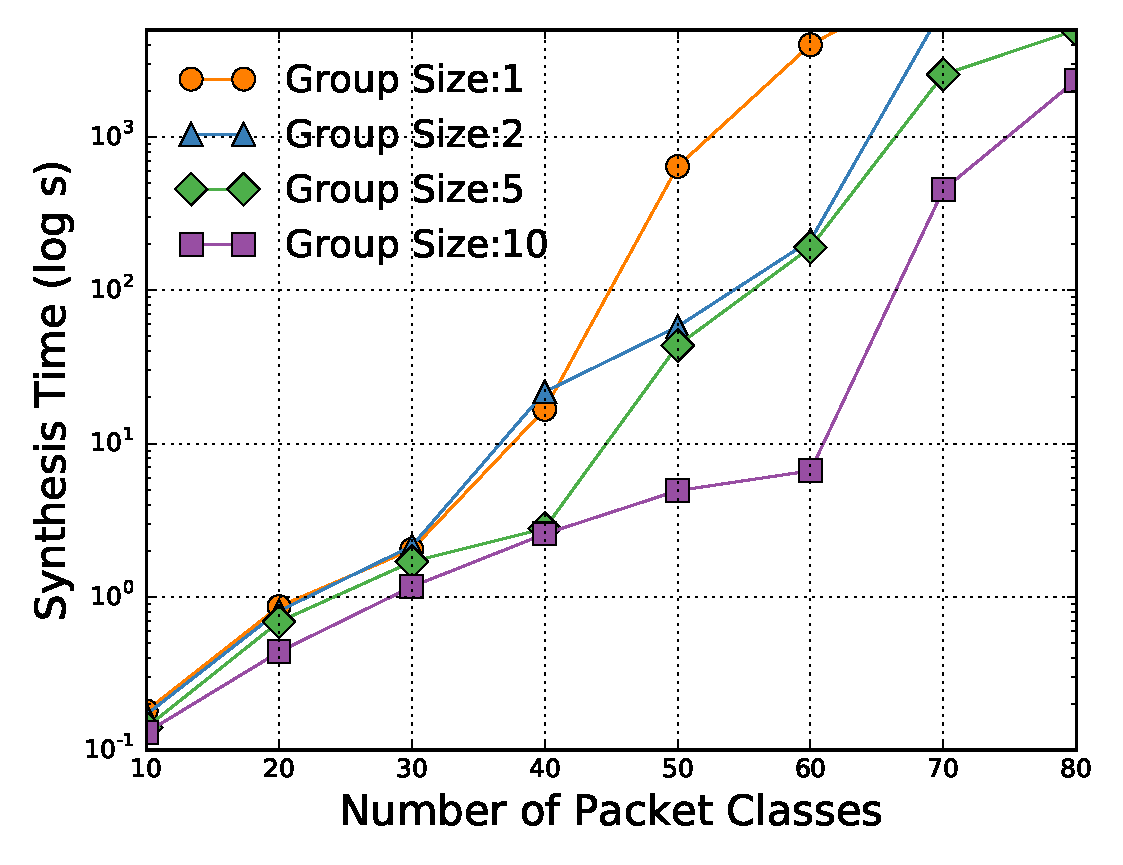
\includegraphics[width=0.66\columnwidth]{figures/noTacticIsolation.eps}}
	\subfloat[No Edge Tactic]{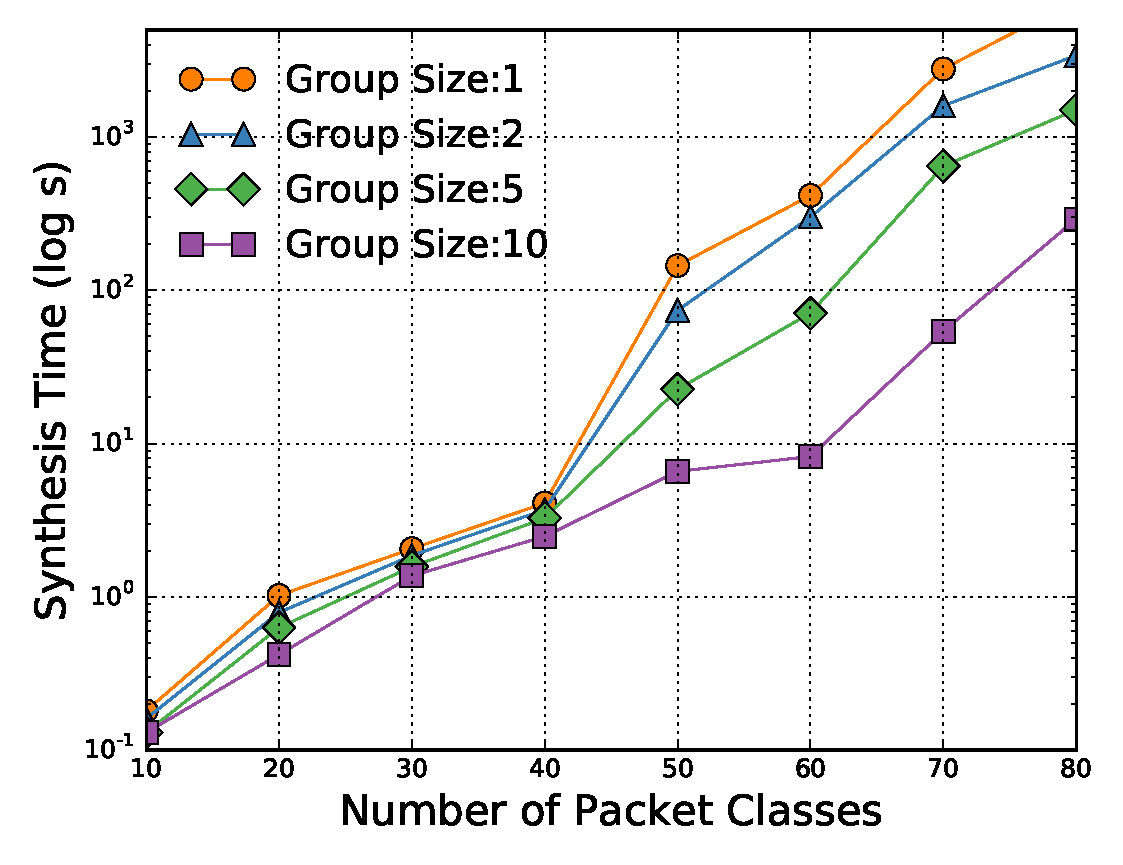
\includegraphics[width=0.66\columnwidth]{figures/edgeTacticIsolation.eps}}
	\subfloat[Valley-free Routing Tactic]{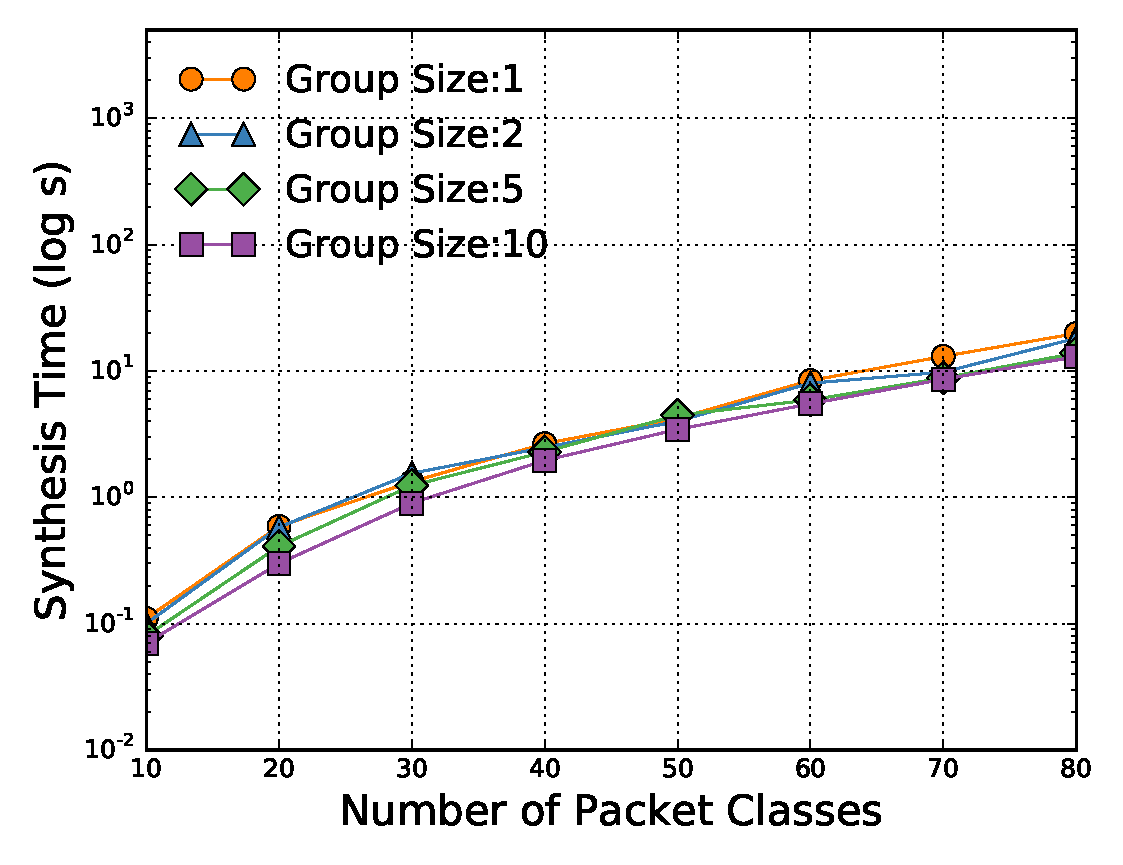
\includegraphics[width=0.66\columnwidth]{figures/noValleyTacticIsolation.eps}}
	\compactcaption{\label{fig:isolation}
		Total synthesis time (log scale) for isolation workloads over range of packet classes and different tenant-group sizes.}
\end{figure*}

\section{Evaluation} \label{sec:evaluation}

We implemented a full working
prototype of \Name in Python. We have implemented an interpreter for
the Genesis Programming Language using PLY~\cite{ply} and the synthesizer using 
the SMT solver Z3~\cite{z3} and its $\nu Z$ extension for MaxSMT and linear
 optimization~\cite{nuz3}; \name outputs the
forwarding rules for the switches, which can be provided as input to a
SDN controller (e.g., Floodlight~\cite{floodlight}) to install over the
network. \Name uses the Metis graph-partitioning library~\cite{metis}
to perform equi-sized partitioning 
used by divide-and-conquer synthesis. 
%We plan to make the code for \Name publicly available.

In this section, we evaluate \Name using
%\loris{really don't like the word realistic}
enterprise-scale multi-tenant data
center settings. 
Specifically, we ask:
\begin{compactitemize}
\item What is the performance of \Name's baseline synthesis
  algorithm for tenant policies? How does the performance vary with size of the
  network, number and the nature of policies in use? (\secref{sec:baselineeval})
  
  \item What is the performance of \name for operator policies
  like capacity bounds, traffic engineering, and network repair
  which use SMT with linear optimization objectives and MaxSMT? (\secref{sec:optimizationeval})

\item How much do tactics help improve \Name's 
  performance? Which tactics offer the best improvement? (\secref{sec:tacticeval})

\item To what extent does the divide-and-conquer synthesis improve \Name's
  performance? When does it lead to degraded synthesis times? (\secref{sec:optimisticeval})

\end{compactitemize}
%\loris{if you say this here don't write it in the bullet points}
Our experiment settings have a few thousand servers, tens of switches,
and hierarchical fat-tree network topologies which reflect a private
datacenter. Our experiments are parameterized by: (a) total size of
the fat-tree network (45-180 switches), (b) number of
tenants (1-80), and (c) number of packet classes in a tenant (1-10).
Note that a single packet class can be used to specify policy
for multiple host-pairs of a tenant connected to the 
same edge switches, and placement of the hosts can take uniformity
of policy in account to reduce the explosion of packet classes with 
increasing hosts.

Our primary metric of interest is synthesis time, measured in
seconds. In measuring this, we focus on the time the Z3 solver takes
to solve the constraints\footnote{
	We do not account for
constraint generation time in our evaluation, as it 
has polynomial time complexity and thus, can scale well unlike
constraint solving time;
a well-engineered system can considerably reduce
the constraint generation overheads.}. 
All experiments were conducted using a
32-core Intel-Xeon 2.40GHz CPU machine and
128GB of RAM. For evaluating the baseline performance, we impose a
synthetic limit on the path length $\mu$ to be $10$, which is adequate 
for a fat-tree topology with three levels. 

\subsection{Baseline Synthesis Performance for Tenant Policies} \label{sec:baselineeval} 
\minisection{Multi-Tenant Isolation} To evaluate the baseline
performance of \Name, we model a multi-tenant 80 switch
 topology with tenant-isolation in
\Cref{fig:isolation}(a).  For each workload we have $n$ tenants with
group size $g$ which is the number of packet classes for each
tenant. The x-axis shows the total packet classes $n*g$.  Packet
classes of a tenant are not isolated (and they implement simple
reachability within the tenant), while packet classes of different
tenants are traffic-isolated. Thus, no two tenants share a link in
the same direction, and can never
affect each other's performance.  We randomly\footnote{ Smarter
  placement of tenants could speed-up synthesis as tenant endpoints
  would be located closer to each other. The placement algorithm can
  be used to develop specialized tactics.}  place endpoints for the
tenants' packet classes, ensuring that no more than 4 tenants share a
single edge switch.  Operators can aggregate a tenant's traffic from
multiple instances connected to the same switches 
as a single reachability policy and establish
pathways for communication amongst different switches.

For a fixed group size, we observe that the total synthesis time
increases exponentially with number of packet classes.  As
 group size decreases, for the same number of classes, the 
number of tenants increases, increasing the number of isolation policies
and the synthesis times. 
Group size 1 denotes the
extreme case where all flows are isolated with each other.
 
While we evaluated a multi-tenant isolation setting, there are other
scenarios that translate to these workloads. Consider an example where
specific flows of tenants require QoS guarantees and these flows must
be isolated w.r.t. all other flows. This translates to a two-tenant
isolation setting. Operators can provide weaker isolation such that
two flows must be isolated on only certain ``special" links. 
This is an easier problem to tackle than isolation over all
links, and the performance of such scenarios would be better. 
Failure resiliency uses link-isolation policies which exhibit a similar
performance compared to the workloads considered here. 

\minisection{Effect of Topology Size} To evaluate \Name across
increasing topology sizes for isolation workloads, we fix the
tenant-group size to 5, and for each topology, we maintain the ratio
of packet classes to number of edge-aggregate links to 0.25.  We
choose this metric because if we keep the number of classes constant,
as topology sizes increases, it is easier to find isolated
paths due to more links. Thus, by keeping the number of packet classes proportional to
size of the topology, we maintain the relative difficulty of the
workload across topologies.  We show the average synthesis time per
class with increasing topology sizes in
\Cref{fig:tactic-topo} (baseline trace).  We are able to synthesize forwarding rules
for 12 tenants with group size 5 in a 125 switch topology in 124
seconds (avg. 2 seconds per traffic class).
 %Some comment I dont understand.
We also observe that average time per flow increases exponentially
with larger topologies, thus synthesis times are also exponential
\begin{wraptable}{l}{8em}
	\begin{footnotesize}
		\begin{center}
			\begin{tabular}{P{3em}| P{4em}}
				Number of Waypoints & Avg. Synthesis time per Class (s) \\
				\hline
				1 & 0.034\\
				
				2 & 0.138\\ 
				
				3 & 0.983\\ 
				
				4 & 15.41\\ 
				
				5 & 32.93\\
			\end{tabular}
		\end{center}
		\compactcaption{Average synthesis time per class for waypoint policies with increasing number of waypoints. } \label{tab:waypointeval} 
	\end{footnotesize}
\end{wraptable} 
in the number of switches.

\minisection{Waypoint Policies} To evaluate \Name's performance for
ordered sets of waypoints, we fix the number of waypoints (range:1-5)
 and generate 100 waypoint policies with different sizes and permutations
 of the ordered waypoint sets for a 80 switch topology.
 Each policy has edge switches as endpoints and randomly picked core or
aggregate switches for waypoints. The synthetic limit $\mu$ on the
path length is increased to 15 and no tactics are used 
(difficult to devise a tactic for the path satisfying a waypoint policy). The
average synthesis time for a waypoint policy is reported in
\Cref{tab:waypointeval}.  We observe that synthesis time increases
exponentially with total number of waypoints in a packet class's
policy, owing to the complexity of the problem.  \Name can synthesize
rules for a path with 3 total waypoints in less than a second, on
average. 
%\aditya{I don't follow this last sentence}


\subsection{Baseline Synthesis Performance for Operator Policies} \label{sec:optimizationeval}
\minisection{Isolation with Link Capacity Policies}
\Cref{fig:link-capacity} (baseline trace) 
shows the average synthesis time per flow for the same setting as above, but
additionally, there are 10 low-bandwidth links in the network for which the operator
specifies capacity policies (all packet classes have uniform capacity). 
Since we use LRA for link capacity constraints, we see an 
increase in average time for synthesis 
when compared to pure isolation which is completely 
encoded using SAT. 

\minisection{Traffic Engineering} \Cref{tab:optimizeval} 
shows the synthesis time for workloads on a 80-node fat-tree topology
with different traffic engineering (TE) objectives. \name can synthesize a data plane
minimizing average utilization for 200 packet classes in approximately 2000 seconds. 
However, for minimizing the maximum link utilization, 
\name can only synthesize 50 packet classes in close to 4000 seconds. For both
objectives, the synthesis time increases exponentially with the number of packet classes. 
SMT with optimization objectives is an emerging field of research, 
and we envision that solvers in the future will become fast
and handle larger workloads. 

\minisection{Minimal Repair} 
To evaluate the performance of minimal repair using MaxSMT, we
consider a setting with 8 tenants, each with 10
packet classes (total classes=80), and tenant flows are isolated from
one another. Now, we disable the switch with the largest number of
rules, and try to find a new data plane
satisfying the original tenant isolation policies such that the 
number of switches unaffected is maximized. We can
synthesize the minimal repair in nearly 200 seconds on average. 
With repair, the new data plane only changes rules on
 2-3 switches on average, while naive synthesis results in 
 nearly 60 switches being updated, which is very expensive.
 % Write about waypoints
 \subsection{Tactic Reductions} \label{sec:tacticeval}
 We 
 demonstrate the improvements from using tactics for isolation
 workloads with different number of tenants and group sizes on a 
 80 switch topology.
 
 \noindent {\bf ``No Edge" Tactic}: \Cref{fig:isolation}(b) shows the synthesis time for isolation workloads using the no edge tactic 
 $\neg(e .^* e .^* e)$, which has a  best-case speedup of 9.5$\times$ over baseline synthesis.
 Using this tactic, \Name can synthesize forwarding rules for 12 tenants with group size 5 in under 200
 seconds.
  
\noindent {\bf ``Valley-free" Tactic}:  
For the same isolation workloads as above, we use the tactic $\neg (e .^5 .^* e)$ $\wedge \neg (e .^* e .^* e)$
 which ensures {\em valley-free routing}, that is paths are of the form $eacae$. 
 The results are shown in \Cref{fig:isolation}(c). 
 Using this tactic, \Name synthesizes forwarding rules for each workload in under 20 seconds 
 and can achieve a best-case reduction of 400$\times$ compared to synthesis without tactics. 
 \begin{table}
 	\begin{footnotesize}
 		\begin{center}
 			\begin{tabular}{P{7em} | P{13em} | P{4em}} 
 				Workload Type & Description & Time (s) \\ [0.5ex] 
 				\hline 
 				\multirow{2}{*}{minimize-avg-te}& 100 packet classes & 425 \\ [0.5ex]
 				& 200 packet classes & 2002 \\ [0.5ex]
 				\hline
 				\multirow{2}{*}{minimize-max-te} & 25 packet classes & 522 \\ [0.5ex]
 				& 50 packet classes & 4192 \\ [0.5ex]
 				\hline
 				Network repair & 8 tenants, group size 10, tenant-isolation, 1-switch failure & 219 \\ [0.5ex]
 			\end{tabular}
 		\end{center}
 		\compactcaption{Synthesis times for workloads on a 80-node fat-tree topology with different optimization objectives.} \label{tab:optimizeval} 
 	\end{footnotesize}
 \end{table}
 
 \begin{figure}
 		\centering
 	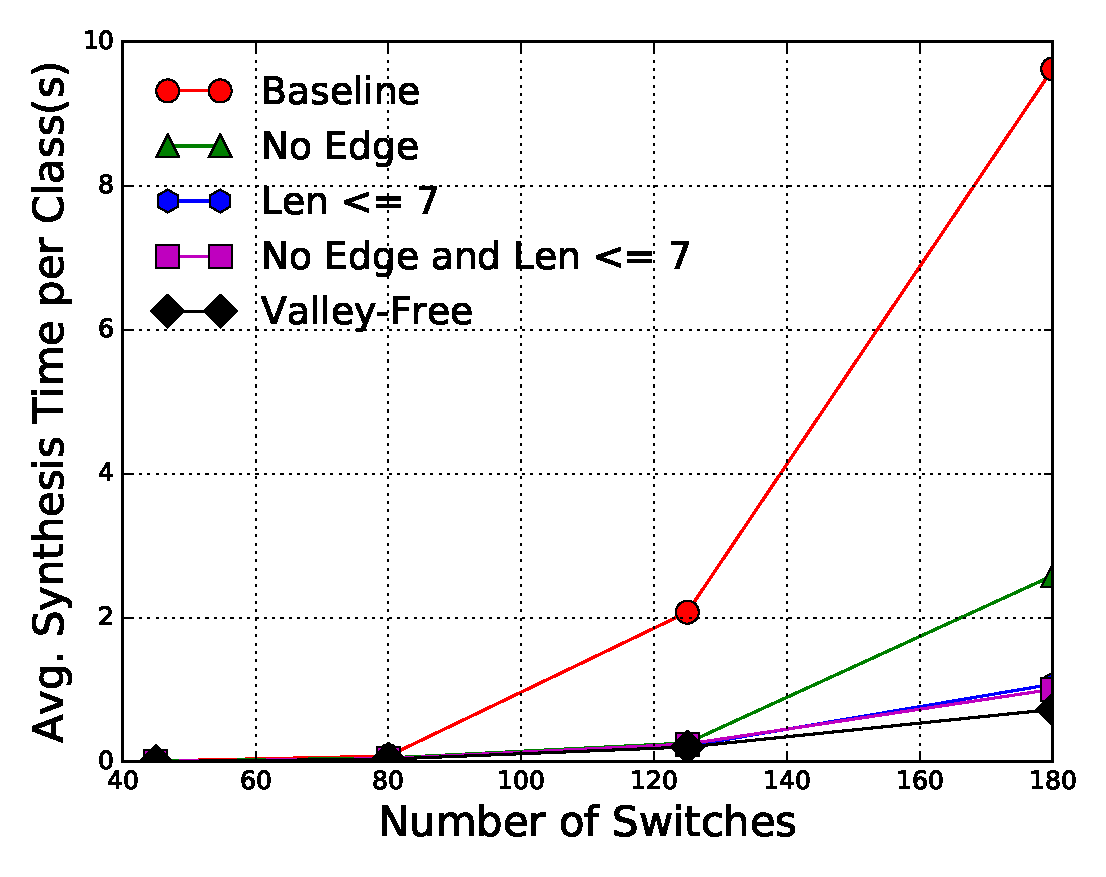
\includegraphics[width=0.65\columnwidth]{figures/isolationTopology.eps}
 	\compactcaption{Average synthesis time per packet class versus topology size for isolation workloads 
 		w/o different tactics with the ratio of packet classes to number of edge-aggregate links 0.25.}
 	\vspace{0.5cm}
 	\label{fig:tactic-topo}
 \end{figure}
 
\noindent {\bf Effect of Topology Size}: 
In \Cref{fig:tactic-topo},
 we evaluate the performance of different tactics for different topology sizes. There is a
 significant reduction in synthesis time for each tactic when compared to the baseline synthesis.
 The performance of each tactic is directly related to the reduction of the search space: more
 restrictive tactics have lower synthesis times. 
  Using the $length \leq 7$ tactic and ``no edge" tactic, \Name synthesizes forwarding rules for 20 tenants of group-size 5 in 100 seconds in a 180 switch
 topology (9$\times$ speedup over synthesis without tactics).
  
 \noindent{\bf Isolation with Link Capacity Policies}: A similar setup
 with additional link capacity constraints for 10 links is evaluated
 using the no edge tactic, and we get a best-case 14$\times$
 improvement over baseline synthesis. 
 Tactics can provide a considerable improvement
 over the baseline performance as illustrated by these experiments,
 and demonstrate the viability of synthesis approach of \Name to
 real-world networks.
 
\subsection{Divide-and-Conquer (DC) Synthesis Performance} \label{sec:optimisticeval} 
To evaluate the divide-and-conquer (DC) synthesis procedure, we
perform 100 runs of DC and non-DC synthesis 
(with the no edge tactic in both cases) on isolation
workloads with varying number of tenants and different group sizes
used in \secref{sec:baselineeval}. We compute the
speedup (time of non-DC synthesis/time of DC synthesis) and plot its
cumulative frequency distribution in \Cref{fig:dcsyn-cdf} to quantify
the benefits of DC synthesis. For more than 80\% of the
workloads, divide-and-conquer offers better or comparable
performance to non-DC synthesis, achieving a speedup of
2$\times$ for nearly 40\% of the workloads. For 20\% of the workloads,
divide-and-conquer performs worse than the non-DC approach,
especially for workloads with tenant group size 1 due to
greater number of recovery attempts. 

%  \aditya{How does this compare to ground up resynthesis? Without a comparison it is not clear minimal repair is useful!}

\minisection{Summary} The key points of our evaluation are:
1) For a representative tenant-group size of 10 in a 80 switch
  fat-tree, the baseline synthesis performance for synthesizing the
  forwarding rules for 1 to 8 tenants with complete tenant-isolation
  is in 0.1-2000s.
2) Operator policies like optimization objectives for TE and  
   network repair is more expensive than synthesis without
   objectives.
3) Tactics provide considerable speedup over the
        baseline synthesis.  We can
        synthesize the above workloads in 0.1-300s using the no edge
        tactic, and under 12s using the valley-free routing tactic.
4) \Name can further benefit from 
        divide-and-conquer (DC) synthesis, which provides a 2.0$\times$ speed-up
        over non-DC synthesis in 40\% of the workloads, in
        addition to the tactic improvements.
 
%!TEX root = paper.tex
\section{Related Work}\label{sec:related}
\minisection{Centralized control}  RCP~\cite{rcp}, supported logically central BGP
configuration. The more recent Fibbing~\cite{fibbing} system provides
centralized control over distributed routing by creating fake nodes
and fake links to steer the traffic in the network through paths that
are not the shortest, similar to how \name uses static routes.  Both
approaches face the issue of forwarding loops in the network during
failures. Fibbing and \name differ in the specific algorithms to solve
the synthesis problem.  \name does offer key advantages: first, by
using static routes for steering, we do not increase the control traffic in
the network, unlike the fake advertisements used in Fibbing. Second,
Fibbing by design targets a single domain and does not take into account
domain decomposition and inter-domain routing. 

%However, these fake advertisements can create
%forwarding loops in the network during failures, and the centralized
%controller has to respond to failures (response to failures can
%precomputed), thus making the controller a central point of
%failure. In contrast, our approach to distributed control plane
%synthesis can provide the same expressive power as Fibbing but avoids
%any centralized component by engineering the control plane parameters
%to match the input specifications.  


\minisection{Configuration synthesis} 
ConfigAssure~\cite{configassure}
uses a combination of logic programming and SAT solving to synthesize
network configurations for security, 
functionality, performance and
reliability requirements specified as constraints; 
but it does not
support any notion of policy- or connectivity-resilience 
or hierarchical domain splitting.  Fortz
et. al~\cite{ospf-te} tackle the problem of optimizing OSPF weights
for performing traffic engineering, but their work is tailor-made
to just this specific problem.
Propane~\cite{propane, propaneat} tackles the specific problem of
synthesizing BGP configurations for concrete and abstract topologies
to ensure network-wide objectives hold even under failures. 
Propane is suited to specify preferences on paths and
peering policies among different autonomous systems. Propane
translates policies to a graph-based intermediate representation,
which is then compiled to device-level BGP configurations. 
\kausik{
The compilation and resilience algorithms for Propane use automata
and are tailored for its underlying technology (BGP configurations with support for 
local preferences, MEDs and communities), in contrast to our LP-based
algorithms which synthesize OSPF and static routing configurations which have
a different forwarding model than BGP.}


SyNET~\cite{synet} tackles network-wide configuration synthesis
(Definition \ref{def:policycompliance}) by
modeling the behavior and interactions of the routing protocols as a
stratified Datalog program, and using SMT to synthesize the Datalog
input such that the fixed point of the Datalog program (which
represents the network's forwarding state after convergence) 
satisfies certain policies or path requirements.  While
both systems can take paths as input requirements, \name uses
a two-phase approach where OSPF weights are synthesized
separately using
LP-solvers---which are faster and parallelizable---rather than directly  
solving the whole configuration synthesis problem using SMT solvers.  
Moreover, SyNET's approach
does not deal with resilience, a key aspect we tackle in this paper,
and SyNET does not attempt to minimize the number of static routes,
which can cause undesirable behaviors like routing loops.  

\minisection{Policy languages} While \name uses \genesis 
to synthesize policy-compliant paths, in the future it could use
other policy language frameworks as a front-end (with 
less rich policy support but better
performance). %% Other works on
%% centralized policy enforcement for SDN are Merlin~\cite{merlin} and
%% NetKAT~\cite{netkat}.
In Merlin~\cite{merlin}, data planes that adhere to policies expressed
using regular expressions and min and max
bandwidth guarantees are synthesized using mixed
integer linear programming (ILP). 
NetKAT~\cite{netkat} is a domain-specific language and logic for 
specifying and verifying network packet-processing functions
for SDN, based on Kleene algebra with tests (KAT). NetKAT can  
express certain network-wide policies like reachability and waypoints.
However, both Merlin and NetKAT do not support link-isolation 
to produce edge-disjoint paths, which is needed for waypoint-compliance in ~\secref{sec:waypointres}.


%% However, the NetKAT semantics
%% cannot be used to express policies based on hyperproperties
%% ~\cite{hyperproperties}, i.e., 
%% the packet processing function requires multiple packet histories
%% as input. Traffic engineering or isolated paths are policies
%% based on hyperproperties.

%% While Genesis supports richer policies, its SMT-based approach is slower in synthesis. As part of future work, we will consider how

%Fine-grained traffic engineering based on online demand/flow size estimation and 
%rapid rerouting is also crucial for datacenter workloads, and extending \name's
%TE policies to fine-grained timescales is subject of future work.
%Also, the performance
%of SMT solvers with optimization objectives is quite slow, and calls for 
%domain-specific techniques to speed up the synthesis. Also, datacenter
%networks are highly symmetrical, and this symmetry can be leveraged
%to speed up synthesis (similar to the work of Plotkin et. al~\cite{symmetry} to
%speed up network verification using symmetry). The main challenges of
%using symmetry in synthesis is considering two aspects of symmetry: network
%symmetry and policy symmetry. Also, our treatment of resilience synthesis
%is preliminary and future work will be geared towards synthesizing resilient
%forwarding planes incorporating capacity constraints and traffic engineering.
 

\section{Conclusion}

We presented \Name, a general and extensible network management system
for enterprise-scale multi-tenant datacenter networks. It allows
rich policies to be specified declaratively. It leverages
the formal reasoning foundations of constraint solving together with
fast SMT solvers to synthesize data plane configuration from high
level policies. This abstracts away the difficult of programming or
configuring individual switches. \Name incorporates novel ideas to
speed up synthesis, leveraging the hierarchical nature of datacenter
network topologies and the structure of the interaction between
tenants' policies. These optimizations help \Name synthesize policies
for realistic settings in a few seconds, making it pratical to use in
network management.

%   Operators in multi-tenant cloud data centers require support for
%   diverse and complex end-to-end policies like reachability, middlebox
%   traversals, isolation, and network resource management. We present
%   \Name, a network management system which allows these policies to be
%   specified in a declarative manner without explicitly programming the
%   data-plane behavior.  \name tackles the problem of enforcing the
%   policies by synthesizing switch forwarding tables. In doing so, it
%   uses the formal reasoning foundations of constraint solving in
%   combination with fast off-the-shelf SMT solvers.  To improve
%   synthesis performance, \Name incorporates a novel search strategy that
%   uses regular expressions to specify properties that leverage the
%   structure of datacenter networks,
% %topologies to specify properties of the path 
%   and a heuristic synthesis procedure which exploits the structure of
%   policy interactions.  Experiments demonstrate the performance of
%   \Name with different workloads on real-world topologies. Overall,
%   the approach used by \Name is general and instrumental to building a
%   comprehensive network management system.

\section*{Acknowledgments}
We thank the anonymous reviewers,
Nate Foster, Aaron Gember-Jacobson, 
Raajay Viswanathan and Brent Stephens 
for their insightful feedback and suggestions. 
Kausik, Loris and Aditya  
are supported by the Wisconsin Institute
on Software-defined Datacenters of Madison and 
grants from Google and National
Science Foundation (CCF-1637516, CNS-1302041, CNS-1330308, CNS-1345249).

\bibliographystyle{ACM-Reference-Format}
\bibliography{references}

\appendix
\section{Proofs}
\begin{theorem}[Hardness of synthesis]
\label{thm:ospfsynth}
Given a
network with a single domain,
and a positive number $C_{sc}$,
the problem generating
a path-compliant configuration with at most $C_{sc}$ static routes
is NP-complete.
\end{theorem}
%!TEX root = paper.tex
\begin{proof}
We show that the decision version of the minimum 
vertex cover problem, i.e., there exists a vertex cover
of size $ \leq k$, which is NP-complete, 
reduces to finding a set of static routes 
of size $ \leq k$ \
and OSPF weights for a network with only one domain. 
The latter is also in NP, so after the reduction we 
can conclude that it is also NP-complete.

Let $G = (V,E)$ be an instance of the 
minimum vertex cover problem. A set of
vertices $VC \subseteq V$ is the vertex cover
if $\forall (v_1, v_2) \in E. ~v_1 \in VC \vee v_2 \in VC$. 

We now show how to construct a topology $T=(S,L)$ 
and a corresponding set of paths $\Pi$ that can be enforced 
by configuration C which requires static routes $SR$ such that $|SR| \leq k$  
if and only if the corresponding $VC(SR)$ is a vertex cover of 
the graph $G$ and $|VC(SR)| \leq k$.

\paragraph{Construction.}
For every vertex $v \in V$: add a vertex $r_v$.
For every edge $(u,v) \in E$: add two vertices $s_{uv}$
and $t_{uv}$ to $S$. Add edges
connecting $s_{uv} \rightarrow r_{u}$, $s_{uv} \rightarrow r_{v}$,
$r_{u} \rightarrow t_{uv}$ and $r_{v} \rightarrow t_{uv}$. 
\Cref{fig:rfcomplexity} illustrates this construction.
\begin{figure}[H]
	\centering
	\begin{tikzpicture}[shorten >=0.5pt,node distance=1.5cm,on grid,auto,
	square/.style={regular polygon,regular polygon sides=4}] 
	\node[state] at (0,0) (s)  {$s_{uv}$}; 
	\node[state] at (3,-1) (v)  {$r_v$}; 
	\node[state] at (3,1) (u)  {$r_u$}; 
	\node[state] at (6,0) (t) {$t_{uv}$}; 	
	\node[state] (s1) [below=of s] {$s_{vw}$}; 	
	\node[state] (t1) [below=of t] {$t_{vw}$}; 	
	\path[-] 
	(s) edge  node {} (v)
	edge  node {} (u)
	edge [blue, dashed, bend right=40] node {} (t)
	edge [red, dashed, bend left=40] node {} (t)
	(u) edge node {} (t)
	(v) edge node {} (t)
	edge node {} (t1)
	edge node {} (s1);
	\path[->]
	(s)
	edge [blue, dashed, bend right=40] node {} (t)
	edge [red, dashed, bend left=40] node {} (t);
%	\path[-] (s) edge node[above] {} +(1,-0.1);
%	\path[-] (t1) edge node[above] {} +(-1,-0.1);
	\end{tikzpicture}
	\caption{Construction for reduction to Vertex Cover.}
	\label{fig:rfcomplexity}
\end{figure}
If there is another edge $(v,w) \in E$, then
$s_{vw}$ and $t_{vw}$ have an edge connecting to $r_v$ (shown
in \Cref{fig:rfcomplexity}). 

For each edge $(u,v) \in E$, we add two paths in $\Pi$: 
$s_{uv} \rightarrow r_u \rightarrow t_{uv}$
for destination host $d_u$ and 
$~s_{uv} \rightarrow r_v \rightarrow t_{uv}$ 
for destination host $d_v$.
(dashed paths in \Cref{fig:rfcomplexity}). 

We now prove that if there exists a set of static routes
$SR$ such that $|SR| \leq k$ such that the resulting configurations
are path-compliant for $\Pi$, then there exists a vertex cover $VC$
of $G$ such that $|VC| \leq k$. 

For each static route $sr \in SR$, the static route
has to be placed at the source, either going to $r_u$
or $r_v$ (structure of topology $T$). 
We construct a set $VC(SR)$ by adding the vertex $v$
based on the endpoints of each static route $sr \in SR$.
To show that $VC(SR)$ is a vertex cover of $G$, we first
prove \Cref{lemma:diamond}.

\begin{lemma} \label{lemma:diamond}
	 For each diamond formed by the input paths, atleast 1 
	 static route on one of the edges of the paths of the diamond 
	 is required to find a valid solution to the
	 OSPF edge weights.  
\end{lemma}

\begin{proof}
Given two paths $\pi_1$ and $\pi_2$ for destinations 
$d_u$ and $d_v$, we define these paths form a diamond
if these paths intersect at two routers ($s_{uv}$ and $t_{uv}$) 
without any common router in between. 
Consider the following diamond % in \Cref{fig:diamond}
constructed by paths $\pi_1$: $s_{uv} \rightarrow r_u \rightarrow t_{uv}$ 
for destination $d_u$ and $\pi_2$: $s_{uv} \rightarrow r_v \rightarrow t_{uv}$ 
for destination $d_v$. Let us assume there exists a solution 
for the OSPF edge weights without any static routes. 

We add the following inequality 
to make $\pi_1$ is the shortest 
path from $s_{uv}$ to $t_{uv}$ by
ensuring
 $\pi_1$ is shorter than the
path from $s_{uv}$ to $t_{uv}$ via $r_v$: 
\begin{equation} \label{eq:diamond1}
	W(s_{uv},r_u) + W(r_u, t_{uv}) < W(s_{uv}, r_v) + W(r_v,t_{uv})
\end{equation}
Since $\pi_2$ is also the shortest path from $s_{uv}$ 
to $t_{uv}$, the linear inequality added is:
\begin{equation}  \label{eq:diamond2}
W(s_{uv},r_v) + W(r_v, t) < W(s_{uv}, r_u) + W(r_u,t_{uv})
\end{equation}
Since there are no static routes on the edges
of $\pi_1$ and $\pi_2$, none of the above equations are 
eliminated. 
Adding equations \ref{eq:diamond1} and  \ref{eq:diamond2} 
yields the inequality $0 < 0$, which is inconsistent 
and therefore, no solution to 
the edge weights exists for this system of equations, 
which contradicts our assumption. Therefore,
for each diamond formed by the input paths, atleast 1 
static route on one of the edges of the paths of the diamond 
is required to find a valid solution to the
OSPF edge weights.  
\end{proof}

For every edge $(u,v) \in E$, the constructed paths from 
$s_{uv}$ to $t_{uv}$ form a diamond. Thus, by Lemma~\ref{lemma:diamond}, 
the diamond created by the paths corresponding to each edge in $G$ 
requires atleast one static route to eliminate
the inconsistency caused by the diamond. If a static route's endpoints
contains $r_u$, we put $u$ in $VC(SR)$ and similarily for $r_v$. 
Edge $(u,v)$ is covered since atleast one static route is added,
thus, atleast one of $\{u,v\}$ is in $VC(SR)$.  
Thus, if $SR$ eliminates all diamond inconsistencies
to find a solution to the OSPF weights, the corresponding set
$VC(SR)$ covers all edges in $E$. Therefore, $VC(SR)$ is a vertex
cover. 

Thus, by finding a set of static routes $SR$ such that $|SR| \leq k$
such that all the diamond inconsistencies are eliminated, and there
exists OSPF weights $W$ such that the configurations forward traffic
along $\Pi$, we can find a vertex cover $VC$ for graph $G$ such that
$|VC| \leq k$. 

This transformation is polynomial, the constructed 
network topology $T$ has $|V| + 2|E|$ nodes, 
$4|E|$ links and $2|E|$ paths. Therefore, OSPF
configuration synthesis with number of static routes $\leq k$ is
NP-complete. Thus, OSPF synthesis with minimal number of 
static routes is NP-hard. 
\end{proof}


\begin{theorem}
	Given a
	network and  set of paths  $\Pi$,
	the problem of generating a domain assignment for which
	there exists a 
	configuration that is path-compliant with $\Pi$ with no static routes
	is NP-complete.
\end{theorem}
\begin{proof}
We show the $k$-graph coloring problem, which is NP-complete
reduces to finding a domain assignment such that the number
of static routes is 0. 
The latter is also in NP, so after the reduction we 
can conclude that it is also NP-complete.

Let $G = (V,E)$ be an instance of the 
$k$-graph coloring problem. Formally, 
we need to find a coloring $C: V \mapsto \{1,2,\ldots k\}$
such that for $\forall (u, v) \in E. C(u) 
\not= C(v)$.

\begin{figure}[H]
	\centering
	\begin{tikzpicture}[shorten >=0.5pt,node distance=1.5cm,on grid,auto,
	square/.style={regular polygon,regular polygon sides=4}] 
	\node[state] at (0,0) (s)  {$r_u$}; 
	\node[state] at (2,-0.75) (v1)  {$d_1$}; 
	\node[state] at (2,0.75) (u1)  {$d_2$};
	\node[state] at (4,0) (t) {$r_v$};
	\path[->] 
	(s) edge [red] node {} (v1)
	edge  [blue]  node {} (u1)
	(u1) edge [blue] node {} (t)
	(v1) edge [red] node {} (t);
	\path[-] 
	(s) edge node {} (t);
	\end{tikzpicture}
	\compactcaption{Construction}
	\label{fig:domasscomplexity}
\end{figure}

Let us consider a network topology $T = (R,L)$. 
For each $v \in V$, add a router $r_v \in R$. To
ensure any domain assignment to the $r_v$'s is valid, we 
add edges to connect every router. 

For every edge $(u, v) \in E$, we construct a
$(u, v, \lambda_1, \lambda_2)$-$diamond$ (Section 6.2) %TODO
as illustrated in \Cref{fig:domasscomplexity}. For every
edge $(u, v) \in E$, we add $d_1, d_2$ to R, and add
paths: $u \rightarrow d_1 \rightarrow v$ and 
 $u \rightarrow d_2 \rightarrow v$ to $\Pi$. 
 
Suppose we find a domain assignment $\Theta$ 
with $k$ domains such that number of static routes is zero. 
Since, the count of static routes is 0, 
for two routers $r_u, r_v$ which 
have a diamond, $\Theta(r_u) \not= \Theta(r_v)$. This is
because, if $\Theta(r_u) = \Theta(r_v)$, then atleast 
one static route would be required to eliminate the diamond. 
Therefore, for every edge in $(u,v) \in E$, 
the routers $r_u$ and $r_v$ belong to 
different domains, therefore $u$ and $v$ have different colors. 
There, the $k$-graph coloring problem reduces to finding 
a domain assignment with zero static routes.  
Therefore, the policy-compliance synthesis problem is NP-complete.
\end{proof}






%% Appendix

\end{document}
